% Seleziona la classe usata per il documento con le opzioni che vogliamo
\documentclass[a4paper, 11pt, twoside, openright]{book}
% Codifica del testo
\usepackage[utf8]{inputenc}
% Lingue usate nel testo, l'ultima e' la lingua principale
\usepackage[english, italian]{babel}
% Tipo di caratteri utilizzare nell'output (pdf e dvi).
\usepackage[T1]{fontenc}
\usepackage{type1ec}
% Pacchetto che permette di creare il frontespizio della tesi
\usepackage[signatures]{frontespizio} % signatures = nel campo dei relatori/correlatori viene lasciato lo spazio per le firme
% Per avere la lettera di inizio capitolo grande.
\usepackage{lettrine}
\usepackage[autostyle, italian=guillemets]{csquotes}
\usepackage{acronym}
% Serve per inserire codice complesso nel testo
% Per codice molto semplice ed in linea possiamo usare il
% l'ambiente o il comando verbatim
\usepackage{listings}
% Gestisce la bibliografia
\usepackage[sorting=none, citestyle=numeric, backend=biber]{biblatex}
\usepackage{graphicx}
\usepackage[usenames,dvipsnames,svgnames,table]{xcolor}
% Per gli indici dei capitolo, sezioni ecc. in caso volessimo metterli
\usepackage{minitoc}
% Permette di inserire delle sotto-figure
\usepackage[font=small]{caption}
%\captionsetup{width=.8\linewidth} % modifica dimensioni intestazione
\usepackage{subcaption}

%\usepackage{siunitx}
\usepackage{emptypage}

% Verbatim in caption
\usepackage{fancyvrb}

\newcommand{\Csh}{C
\includegraphics{hash-symbol}}


%\usepackage{enumitem}

\addbibresource{bibliography.bib}

% Imposta lo spazio fra le linee del testo
\linespread{1,2}

\newcommand{\Csharp}{%
    {\settoheight{\dimen0}{C}C\kern-.05em \resizebox{!}{\dimen0}{\raisebox{\depth}{\bf \#}}}  
}

% ********************************************************************
% listings
% ******************************************************************** 
\renewcommand{\lstlistingname}{Codice}% Listing -> Algorithm

%------------------%
% MINITOC settings %
%------------------%

\dominitoc % Indice per ogni capitolo
% Questi di solito li lascerei commentati altrimenti
% l'indice per capitolo diventa troppo complesso e con troppe cose.
% \dominilof % Lista delle figure per ogni capitolo
% \dominilot % Lista delle tabelle per ogni capitolo

% impostazioni per codice listings (preso da documento Andrea)
\definecolor{stringColor}{HTML}{a31515} % for strings
\definecolor{commentColor}{HTML}{008000} % comments
\definecolor{keywordColor}{HTML}{0000ff} % keywords
\definecolor{stringDocColor}{HTML}{a31515} % javadoc

\definecolor{moreKey1Color}{HTML}{af00db} % keywords
\definecolor{moreKey2Color}{HTML}{267f99} % keywords
\definecolor{regionColor}{HTML}{b4b4b4} % regions

\definecolor{blightgray}{rgb}{0.98,0.98,0.98}

\lstset{
    captionpos=t,
	basicstyle={\scriptsize\ttfamily},
% 	numbers=left,
% 	numberstyle=\tiny\color{black},
	backgroundcolor=\color{blightgray},
	showstringspaces=false,
	columns=flexible,
	stringstyle={\color{stringColor}},
	commentstyle={\color{commentColor}},
	keywordstyle={\color{keywordColor}},
	frame=single,
	framesep=5pt,
	breaklines=true,
	rulecolor=\color{lightgray},
	flexiblecolumns=true,
	xleftmargin=2pt,
	breakatwhitespace=true,
	tabsize=4,
	showspaces=false,
	showstringspaces=false,
	%% escapeinside={(*@}{@*)},
} 


\lstset{
	basicstyle={\scriptsize\ttfamily},
% 	numbers=left,
% 	numberstyle=\tiny\color{black},
	backgroundcolor=\color{blightgray},
	showstringspaces=false,
	columns=flexible,
	stringstyle={\color{stringColor}},
	commentstyle={\color{commentColor}},
	keywordstyle={\color{keywordColor}},
	frame=single,
	framesep=5pt,
	breaklines=true,
	rulecolor=\color{lightgray},
	flexiblecolumns=true,
	xleftmargin=2pt,
	breakatwhitespace=true,
	tabsize=4,
	showspaces=false,
	showstringspaces=false,
	%% escapeinside={(*@}{@*)},
}
\lstset{
    emph={%  
    region, endregion%
    },emphstyle={\color{regionColor}\bfseries}%
}%
\lstdefinestyle{sharpc}{
    classoffset=0,
    morekeywords={try, catch, throw},keywordstyle=\color{moreKey1Color},
    classoffset=1,
    morekeywords={spdlog, std},keywordstyle=\color{moreKey2Color},
    classoffset=0
}
 % importa il file "settings.tex"


%%%%%%%%%%%%%%%%%%%%%%%%%%%%%%%%%%%%%%%%%%%%%%%%%%%%%%%%%%%%%%%%%%%%%%%%%%%%%
\begin{document} % INIZIO DOCUMENTO %%%%%%%%%%%%%%%%%%%%%%%%%%%%%%%%%%%%%%%%%
%%%%%%%%%%%%%%%%%%%%%%%%%%%%%%%%%%%%%%%%%%%%%%%%%%%%%%%%%%%%%%%%%%%%%%%%%%%%%

%--------------%
% FRONTESPIZIO %
%--------------%
%%%%%%%%%%%%%%%%%%%%%%%%%%%
% FRONTESPIZIO - ITALIANO %
%%%%%%%%%%%%%%%%%%%%%%%%%%%

% per ricompilare il frontespizio bisogna prima cancellare i file di log:
% icona del documento in alto a destra vicino a "Ricompila" > icona del cestino

\begin{frontespizio}

	\Universita{Bologna}
	\Istituzione{Alma Mater Studiorum -- Università di Bologna}
	\Facolta{Ingegneria e Architettura}
	\Scuola{Scuola di Ingegneria e Architettura}
	\Corso[Laurea]{Ingegneria Informatica}
	\Dipartimento{Informatica - Scienza e Ingegneria (DISI)}
	%\Divisione{nome}
	\Titoletto{Tesi di laurea \\
		in \\
		Tecnologie Web}
	\Titolo{Progetto di Applicazioni e Giochi Multiplayer\\
	    su Architettura Unity DOTS}
	\Candidato{Michele Righi}
	\Relatore{Prof.~Paolo Bellavista}
	\Correlatore{Dott.~Andrea Garbugli}
	\Annoaccademico{2019-2020}
	\Piede{Anno Accademico 2019-2020 \\
		Sessione III}

\end{frontespizio}            % Frontespizio
\IfFileExists{\jobname-frn.pdf}{}{\immediate\write18{pdflatex \jobname-frn}} % comandi per la generazione del frontespizio

\null\vspace{\stretch{3}}
\begin{flushright}
\emph{Ai miei nonni Bruno e Anna,\\
instancabili sostenitori del mio percorso di studi}
\end{flushright}
\vspace{\stretch{1}}\null


% Imposta i numeri romani per le pagine 
% del sommario e dei vari indici
\cleardoublepage
\pagenumbering{roman}
\setcounter{page}{1}

%----------------%
% RINGRAZIAMENTI %
%----------------%

%----------%
% SOMMARIO %
%----------%
\chapter*{Sommario}




Con lo sviluppo dell'industria videoludica e della tecnologia, per poter competere con colossi come Unreal Engine di Epic Games, è nata anche per Unity la necessità di una rivoluzione del proprio game engine.
L'elaborato si propone di fornire un background sull'evoluzione generale dei motori di gioco. In seguito, mostreremo le potenzialità offerte dalla nuova tecnologia ``DOTS'' del game engine di \emph{Unity Technologies}. A tal proposito, analizzeremo i principali package di tale architettura. Inoltre, tramite lo sviluppo di un prototipo, svolgeremo un'analisi qualitativa delle prestazioni, mettendo in luce i principali vantaggi che questa offre e traendo le relative conclusioni.

    % Sommario

%------------------------%
% INDICI (TOC, LOF, LOT) %
%------------------------%
% TOC = TableOfContents
% LOF = ListOfFigures
% LOT = ListOfTables

\tableofcontents    % Indice generale

%\listoffigures      % Elenco delle figure

    % Indici

% Imposta i numeri arabi per il resto
% del contenuto di tesi
\cleardoublepage
\pagenumbering{arabic}

%----------%
% CAPITOLI %
%----------%
\mainmatter % numera le pagine coi numeri arabi ripartendo da 1
\chapter*{Introduzione} % l'asterisco fa in modo che non compaia "Capitolo 1"
\addcontentsline{toc}{chapter}{Introduzione} % aggiunge il capitolo al TOC

Per diverso tempo Unity ha lavorato per migliorare le prestazioni del proprio motore di gioco, ma il problema principale non era del motore in sé, quanto più l'approccio con cui veniva scritta la logica delle applicazioni. Infatti, la programmazione orientata agli oggetti (con i classici GameObject e MonoBehaviour), si basa su un design poco performante, non ottimizzabile e decisamente non scalabile.
Dunque, negli ultimi anni gli sviluppatori Unity hanno iniziato una profonda ristrutturazione dell'architettura del loro motore di gioco, modificando quella che era un'architettura basata sugli oggetti, in una nuova, che prende il nome di Data-Oriented Technology Stack (DOTS).

L'obbiettivo di DOTS è riassumibile in \emph{performance by default}. L'idea su cui si basa è che il primo istinto quando si crea qualcosa su Unity dovrebbe essere una buona approssimazione di basso livello della giusta soluzione; e non qualcosa di distaccato su cui bisognerebbe ragionare e che per essere migliorata dev'essere ripensata, ricostruita o buttata via in parte appunto perché non funzionale o performante.
Con un approccio orientato agli oggetti questo non succede (e non può succedere) proprio perché esiste un livello di astrazione che distacca ciò che vediamo e usiamo, da ciò che si trova sotto (l'effettiva realizzazione), per semplificare e rendere tutto ``più simile alla realtà''. Al contrario, con un approccio orientato ai dati, ci si trova già a basso livello, e diventa quindi facile ottenere buone prestazioni e rendere il codice ottimizzabile di default.
In particolare, DOTS permette di sfruttare al meglio i processori multicore, massimizzando le prestazioni delle applicazioni multi-threaded e sfruttando in modo efficiente le cache della CPU. Inoltre, il nuovo approccio orientato ai dati rivoluziona anche il modo di pensare e scrivere il codice, il quale oltre ad avere i benefici delle performance, diventa anche più pulito e organizzato.

DOTS è ancora in fase di sviluppo, infatti le librerie sono soggette a modifiche e vengono aggiornate continuamente, ma è già possibile utilizzarle e accedere alla documentazione ufficiale. Attualmente include i seguenti package: Entities (preview), \Csh{} Job System, Burst Compiler, Unity Physics (preview), Unity NetCode (preview), DSPGraph (experimental), Unity Animation (experimental), DOTS Runtime (preview).


L'obbiettivo dell'elaborato è analizzare principalmente i package Entities e NetCode, che verranno utilizzati per sviluppare un semplice prototipo di videogioco multiplayer. Questo dovrà implementare delle meccaniche di base quali movimento del personaggio e raccolta di oggetti di scena. Il prototipo sarà realizzato interamente mediante l'utilizzo di DOTS, al fine di mostrare i vantaggi offerti da questa architettura.


Nel Capitolo~\ref{cap:evoluzione} forniremo un background sui game engine ed i principali modelli su cui si basano. Dunque, tratteremo il percorso evolutivo che ha portato Unity alla realizzazione dell'architettura DOTS. Nel Capitolo~\ref{cap:ecs} tratteremo il package Entities, che rappresenta le fondamenta di tutto il nuovo design orientato ai dati di Unity. Successivamente, il Capitolo~\ref{cap:netcode} aprirà con un'introduzione ai principali modelli di networking e ai problemi che è necessario risolvere. Dopodiché, mostreremo la soluzione adottata da Unity, tramite i package Transport e NetCode. Nel Capitolo~\ref{cap:prototipo} analizzeremo gli aspetti salienti dello sviluppo del prototipo, spiegando il funzionamento delle classi principali, mentre nel Capitolo~\ref{cap:risultati} svolgeremo un'analisi qualitativa dei principali package dell'architettura, mostrando i risultati sperimentali ottenuti. Infine, nell'ultimo capitolo, forniremo una visione d'insieme dell'elaborato, traendo le relative conclusioni e ragionando sui possibili sviluppi futuri dell'architettura.
   % Introduzione
\cleardoublepage

%\chapter*{Template} % l'asterisco fa in modo che non compaia "Capitolo 1"
\addcontentsline{toc}{chapter}{Template} % aggiunge il capitolo al TOC
\minitoc % Indice del capitolo
% \mtcskip
% \minilof % Lista delle figure
% \mtcskip
% \minilot % Lista delle tabelle


\lettrine{Q}{uesto} e' un template latex per scrivere il documento finale di tesi. In questo capitolo spieghero' brevemente quali sono i pacchetti al momento inclusi in questo template~\marginpar{Questa e' una nota a margine}, insieme ad alcuni dei comandi base utili alla scrittura del documento.


Per i comandi piu' basilari, come: la selezione della classe del documento, stampare l'indice, o aggiungere altri capitoli; fare riferimento al file \verb|main.tex|.

\section{Sezione 1}

\section{Sezione 2}

\subsection{Figure}

\mbox{} serve a non spezzare il contenuto, andando a capo

Questo e' il modo per inserire una sola figura con la caption~\cite{doc:unityengine}

% h = here, t = top, b = bottom, p = page of float
\begin{figure}[!ht]
    \centering
    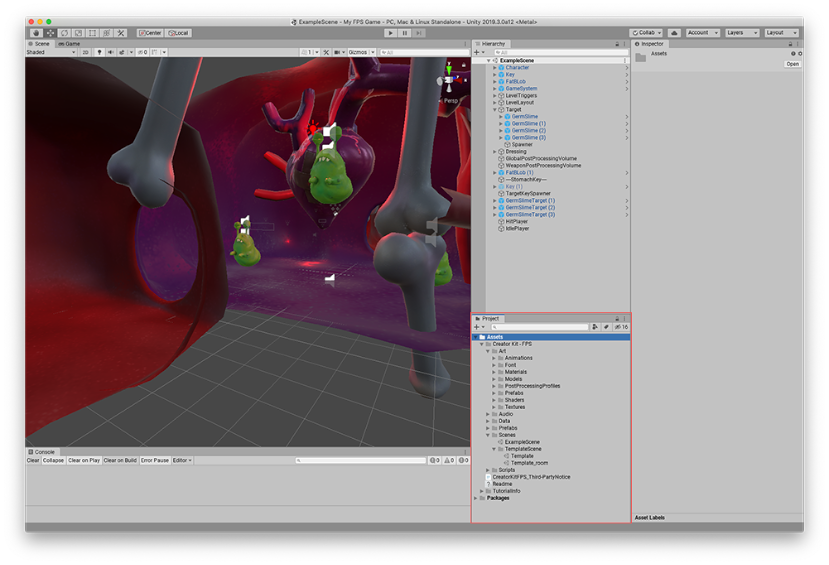
\includegraphics[width=0.95\columnwidth]{gfx/imgs/introduction/unity_editor.png}
    \caption{Unity Engine Editor.}
    \label{fig:unity-engine-editor}
\end{figure}

Mentre questo se vogliamo inserire due figure ognuna con la propria caption:

\begin{figure}[!b]
    \begin{subfigure}{.49\textwidth}
      \centering
      % include first image
      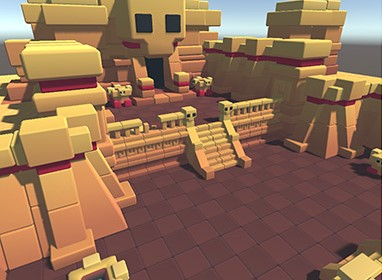
\includegraphics[width=.95\linewidth]{gfx/imgs/introduction/perspective_camera.jpg}
      \caption{Vista in proiezione prospettica.}
      \label{fig:perspective-camera}
    \end{subfigure}
    \begin{subfigure}{.49\textwidth}
      \centering
      % include second image
      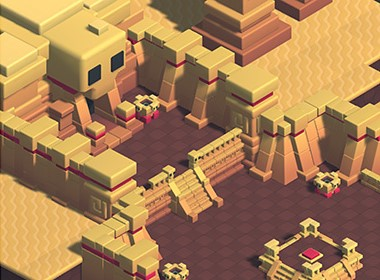
\includegraphics[width=.95\linewidth]{gfx/imgs/introduction/ortho_camera.jpg}
      \caption{Vista in proiezione ortografica.}
      \label{fig:ortho-camera}
    \end{subfigure}
    \caption{Tipi di camera projection.}
    \label{fig:camera-projection}
\end{figure}]


\lstinputlisting{chapters/template.tex} % per importare un file       % Template
%\cleardoublepage

%\setcounter{chapter}{0} % permette di impostare un numero di capitolo differente da quello di default
\chapter{Evoluzione dei Game Engine}
\label{cap:evoluzione}

\section{Background storico}
Nell'ultimo decennio l'industria videoludica si è evoluta notevolmente, soprattutto nel modo in cui i videogiochi vengono realizzati. Oggi infatti, per realizzare un gioco non dobbiamo più scrivere migliaia di righe di codice ma possiamo pensare e lavorare tramite interfacce grafiche e componenti di alto livello. Questo modello di sviluppo è strettamente correlato all'evoluzione dei Game Engine.

L'origine del concetto di Game Engine è da ricercare a metà degli anni '90, principalmente in ambito di giochi 3D o FPS, quando la casa produttrice \emph{id Software} rilasciò un comunicato stampa per annunciare l'uscita di DOOM~\cite{article:hall1992doom}.
Il documento prometteva che il gioco avrebbe «spinto i limiti di ciò che si pensava fosse possibile realizzare su un computer 386sx o migliore», riassumendo diverse innovazioni e tecnologie adottate per implementarlo e, soprattutto, parlava di \emph{DOOM engine}. Inoltre, l'articolo presentava DOOM come un \emph{Open Game}, affermando che la casa produttrice avrebbero fornito la tecnologia ed il supporto per utilizzarla a chiunque l'avesse richiesto.

Questo fu un momento storico molto importante che diede una svolta all'industria videoludica, in quanto per la prima volta si parlò di Game Engine e della separazione dei vari componenti e ambiti nella realizzazione dei giochi. Negli anni successivi il termine è diventato sempre più utilizzato per indicare l'ambiente di sviluppo per progettare e costruire videogiochi (e non solo), composto da vari componenti: rendering grafico, motore fisico, suoni, animazioni, scripting, ecc.
Infatti, analizzando il grafico Google in Figura~\ref{fig:game-engine-google-search} notiamo subito come le ricerche per ``game engine'' si siano impennate proprio negli anni immediatamente seguenti alla pubblicazione di DOOM~\cite{article:lowood2014game}. 
Da quel momento diverse case produttrici hanno deciso di creare un'implementazione proprietaria al fine di utilizzare il game engine per lo sviluppo dei propri videogiochi, mentre società quali ad esempio \emph{Epic Games} e \emph{Unity Technologies} si sono concentrate sulla creazione di un'architettura il più completa possibile e con interfacce user-friendly, che potesse essere utilizzata da tutti, fornendo la relativa documentazione.

\begin{figure}[!ht]
    \centering
    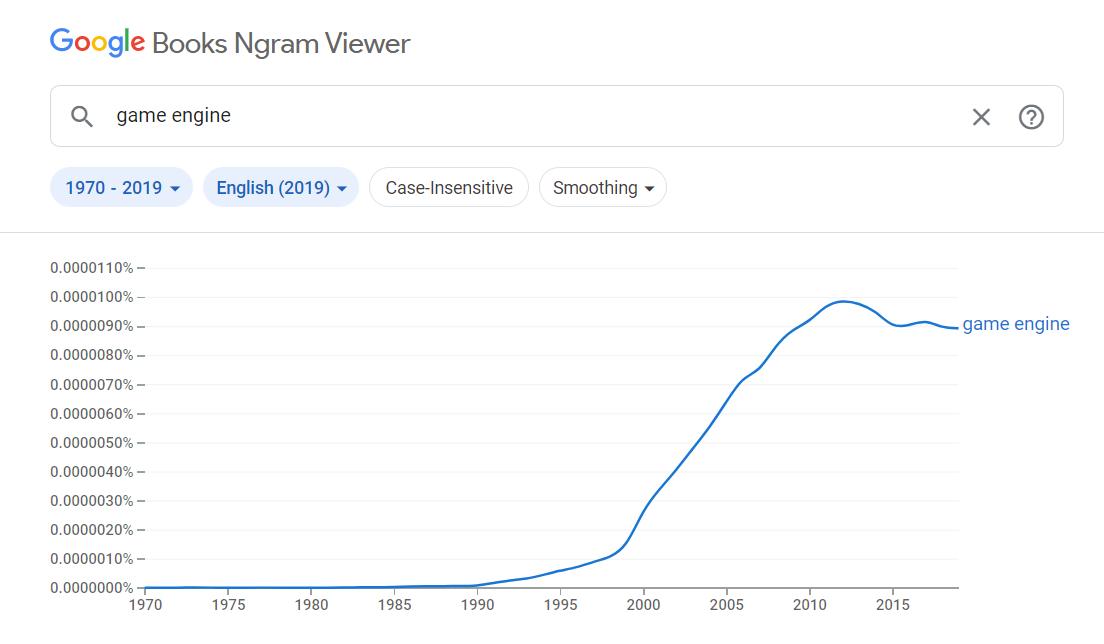
\includegraphics[width=0.95\columnwidth]{gfx/imgs/chapter1/GameEngineGoogleSearch.png}
    \caption{Google Ngram Viewer: ricerche per ``game engine'' negli anni 1970-2019.}
    \label{fig:game-engine-google-search}
\end{figure}

% Game Engine role in game development
%https://momentsonline69.medium.com/the-role-of-game-engines-in-video-game-development-2f1e42e298aa#_=_

\section{Modelli architetturali}
I modelli architetturali adottati nello sviluppo di videogiochi e dai game engine sono riassumibili in tre principali categorie: \emph{inheritance model}, \emph{component-based model} ed \emph{entity component system} (tipicamente abbreviato con ECS).

\subsection{Inheritance model}
Questo pattern è il più tradizionale (molto usato negli anni '90), ed è tipico della programmazione orientata agli oggetti, in cui solitamente è presente una classe, chiamata appunto GameObject, che rappresenta il nodo radice e tutte le classi sottostanti ereditano dati e logica da quest'ultima, creando catene gerarchiche di lunghezza variabile.

L'inheritance model è molto intuitivo e ci permette di semplificare la definizione e la realizzazione di tipi di dato simili, fornendo inoltre la possibilità di sovrascrivere i metodi delle superclassi. Il problema principale di questo modello consiste nel fatto che man mano che i livelli della gerarchia crescono, solitamente perché dobbiamo aggiungere delle entità o delle funzionalità nel gioco, la complessità del codice aumenta con la conseguente diminuzione di riusabilità, flessibilità e, soprattutto, performance. Pertanto, è perfetto per applicazioni e giochi di piccole dimensioni e con poche classi o regole semplici, ma non è assolutamente un modello scalabile~\cite{phd:romeoanalysis}.

\begin{figure}[!ht]
    \centering
    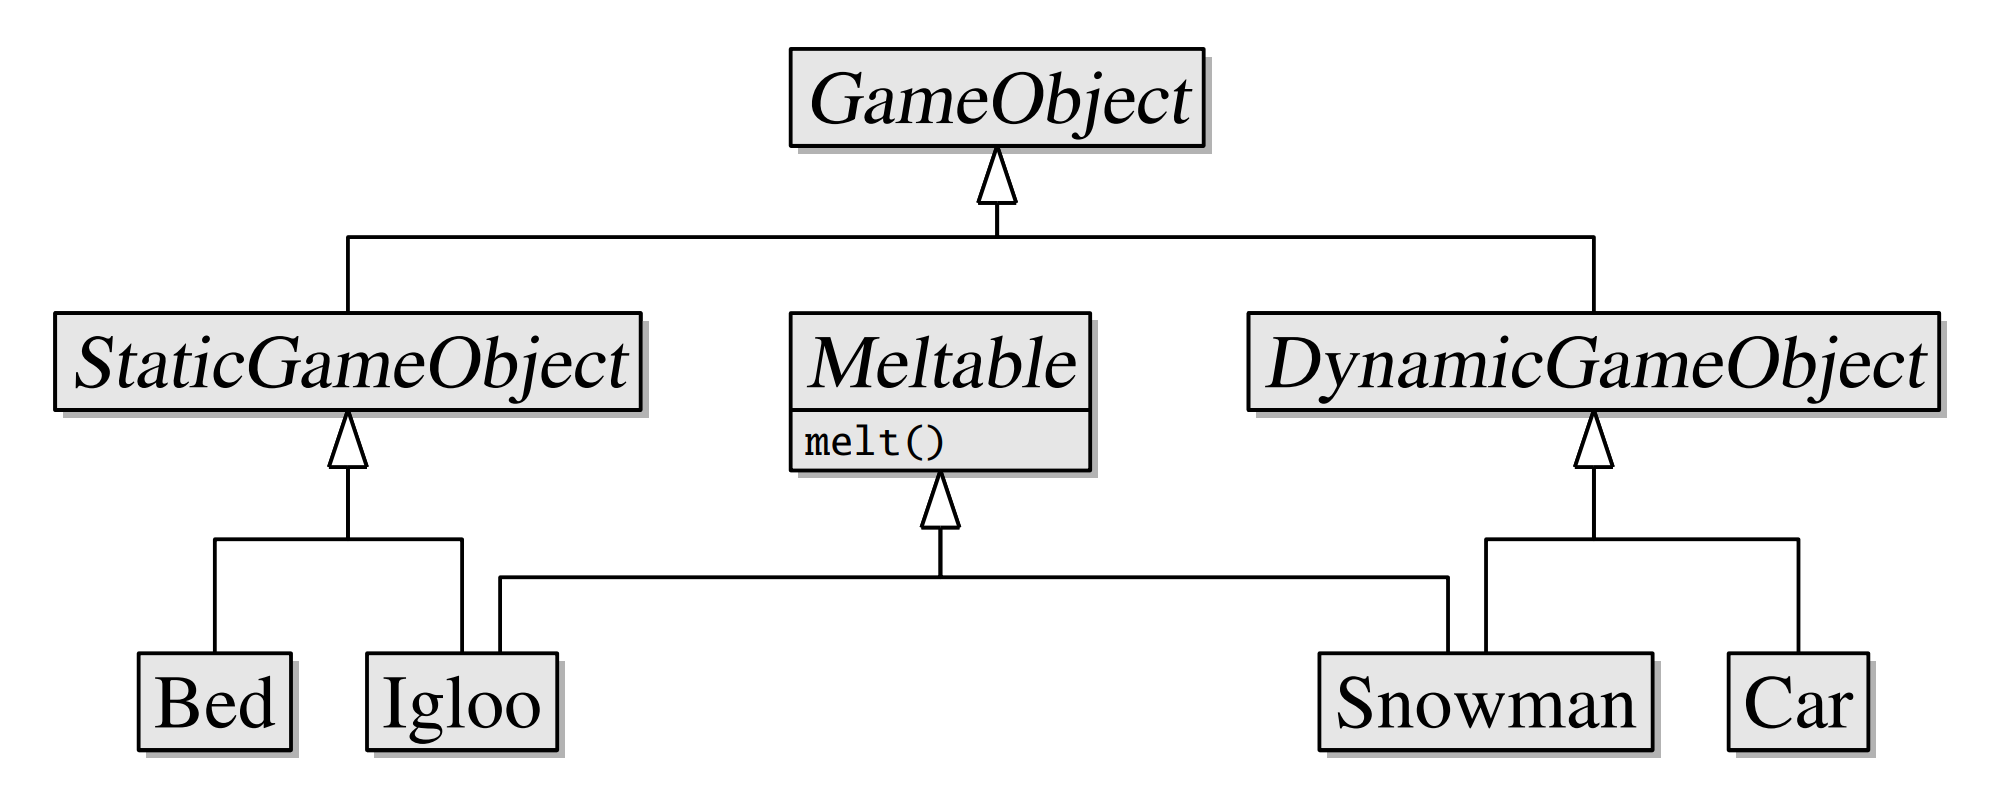
\includegraphics[width=0.95\columnwidth]{gfx/imgs/chapter1/InheritanceModel.png}
    \caption{Esempio: inheritance model~\cite{article:game-architecture-models}.}
    \label{fig:inheritance-model}
\end{figure}

\begin{figure}[!ht] 
    \centering
    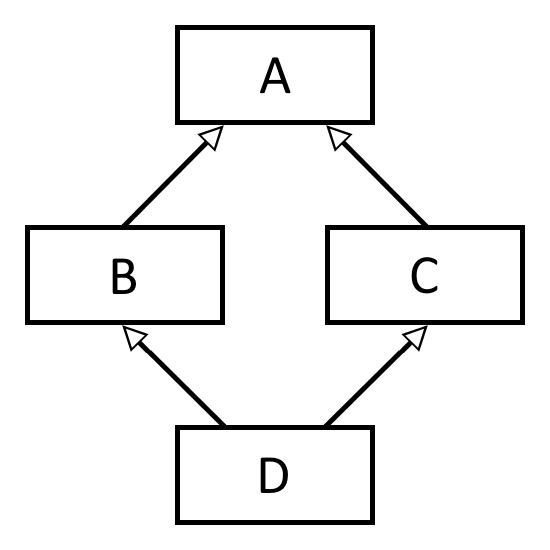
\includegraphics[width=0.50\columnwidth]{gfx/imgs/chapter1/DiamondProblem.png}
    \caption{Problema del diamante.}
    \label{fig:diamond-problem}
\end{figure}

\paragraph{Problema del diamante}
Fra i diversi problemi dell'Inheritance Model, il più famoso è sicuramente il \emph{problema del diamante}, dovuto all'ereditarietà multipla. Se due classi B e C ereditano da una stessa superclasse A, ed una classe D eredita da entrambe B e C, abbiamo ambiguità nel caso la classe D chiamasse un metodo definito in A, in quanto avrebbe due implementazioni diverse (vedi Figura~\ref{fig:diamond-problem}). Per aggirare questo problema, prendendo come esempi i linguaggi \Csh{} e Java, è stato imposto un vincolo secondo cui una classe può ereditare le interfacce da più classi base, ma i metodi ed i dati solamente da una di esse~\cite{article:diamond-problem,itwiki:99605337}.

\subsection{Component-based model}
In un modello basato sui componenti, la gerarchia dei GameObject viene appiattita ad un singolo livello base di GameObject. Quest'ultimo contiene una lista di classi che ne realizzano il comportamento, chiamate componenti.
In questo modo, i GameObject vengono disaccoppiati dal comportamento ed il modello diventa più mantenibile e flessibile, permettendo di creare nuovi tipi di GameObject sfruttando l'aggiunta di ulteriori componenti. Infatti, con questo modello il tipo di un GameObject non è più definito dalla gerarchia di classi a cui appartiene, ma dalla lista di componenti che possiede.

\begin{figure}[!ht]
    \centering
    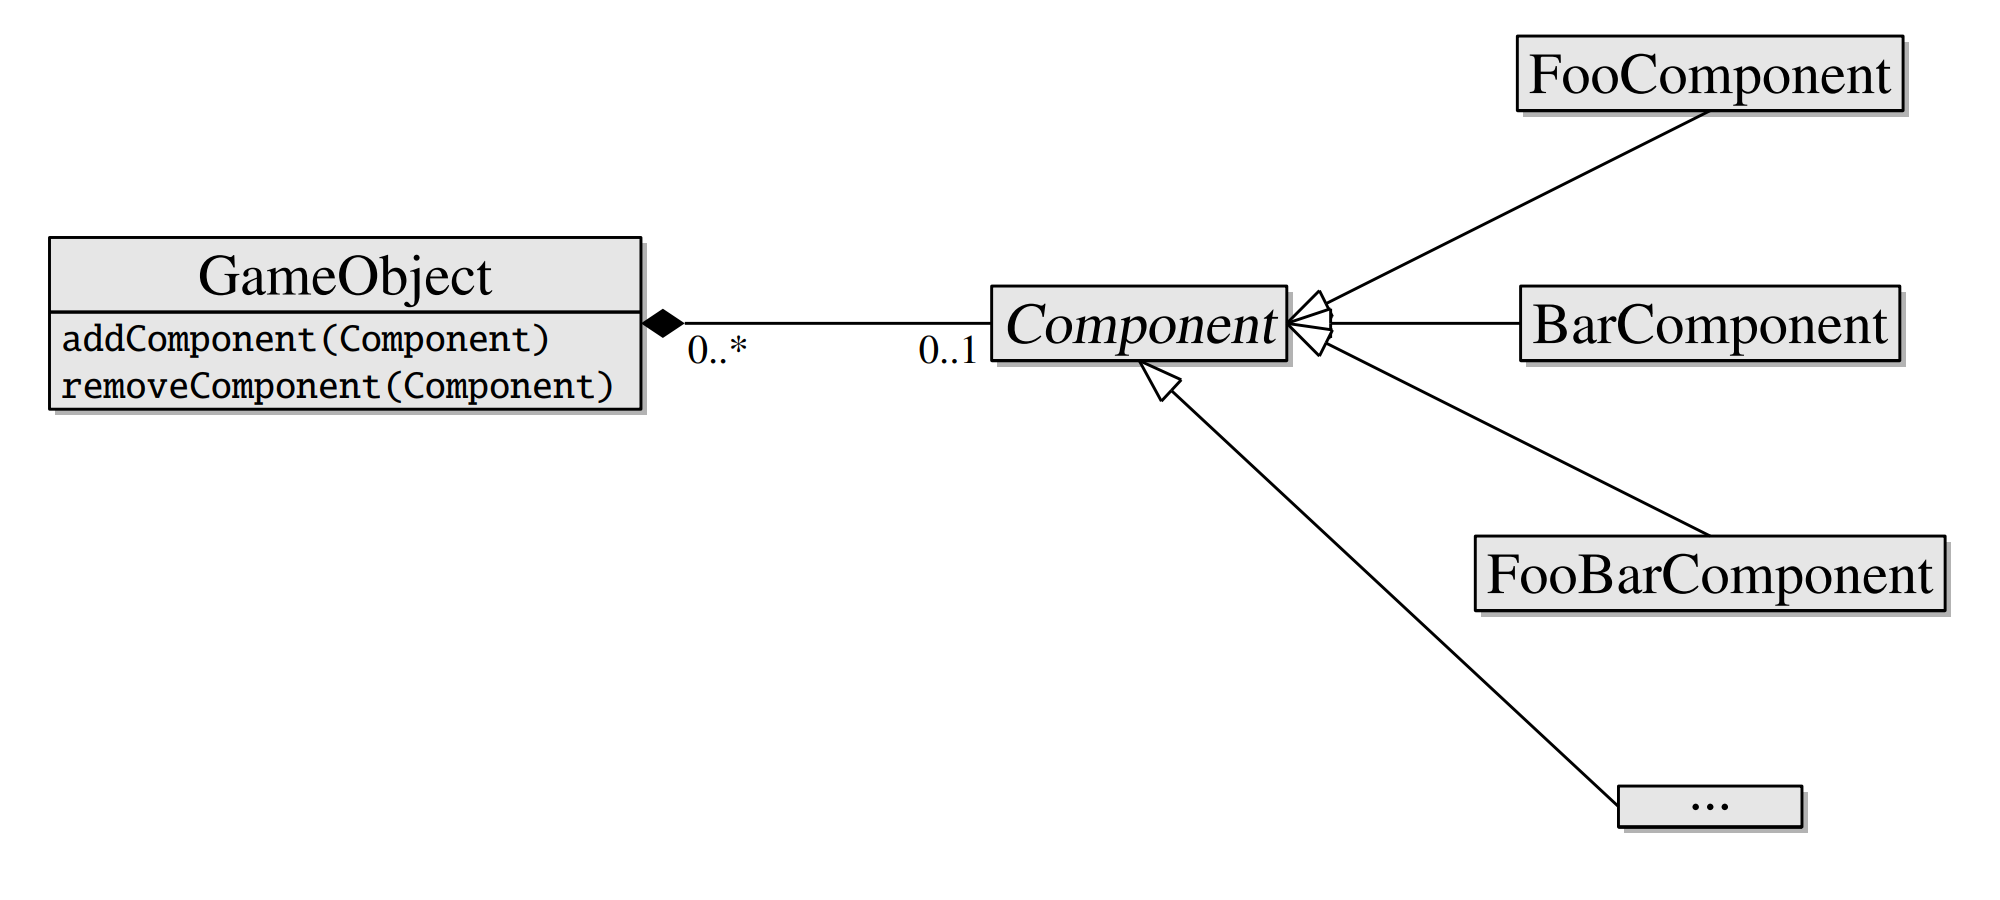
\includegraphics[width=0.95\columnwidth]{gfx/imgs/chapter1/ComponentBasedModel.png}
    \caption{Esempio: component-based model~\cite{article:game-architecture-models}.}
    \label{fig:component-based-model}
\end{figure}

Rispetto al precedente approccio, il component-based model possiede diversi vantaggi, fra cui:
\begin{itemize}
    \item Scalabilità in termini di numero di tipi di GameObject e di comportamento realizzabile per ognuno di essi. 
    \item Modularità dei componenti.
    \item Flessibilità e manutenibilità.
\end{itemize}

Tuttavia, le API dei componenti non sono flessibili ed un loro cambiamento richiede la modifica di tutti i componenti. Infine, i maggiori problemi di questo approccio sono legati all'utilizzo inefficiente di CPU, cache, ed accesso alla memoria~\cite{article:game-architecture-models}.

\paragraph{Utilizzo risorse, CPU e cache}
Sebbene sia un modello migliore del precedente, rimangono comunque molti aspetti che influiscono negativamente sulle prestazioni. In particolare, riguardo l'utilizzo delle risorse, sia inheritance model che component-based model non sono particolarmente ``hardware-friendly''.

Negli ultimi anni, i processori prodotti sono arrivati ad una sorta di velocità limite del clock oltre la quale, per vari motivi~\cite{article:cpu-speed-cap}, non ha più senso spingersi~\cite{article:cpu-evolution}. Di conseguenza, la soluzione migliore per continuare ad ottenere maggiore potenza nelle CPU, è stata quella di aggiungere core (vedi Figura~\ref{fig:cpu-evolution}). Tuttavia, nello sviluppo dei videogiochi spesso solamente uno, massimo due core, vengono sfruttati molto intensamente. Questo solitamente accade perché motori di gioco basati su questo modello architetturale mal supportano la programmazione multithreading. Di conseguenza, il carico sulla CPU non viene bilanciato adeguatamente.

\begin{figure}[!ht]
    \centering
    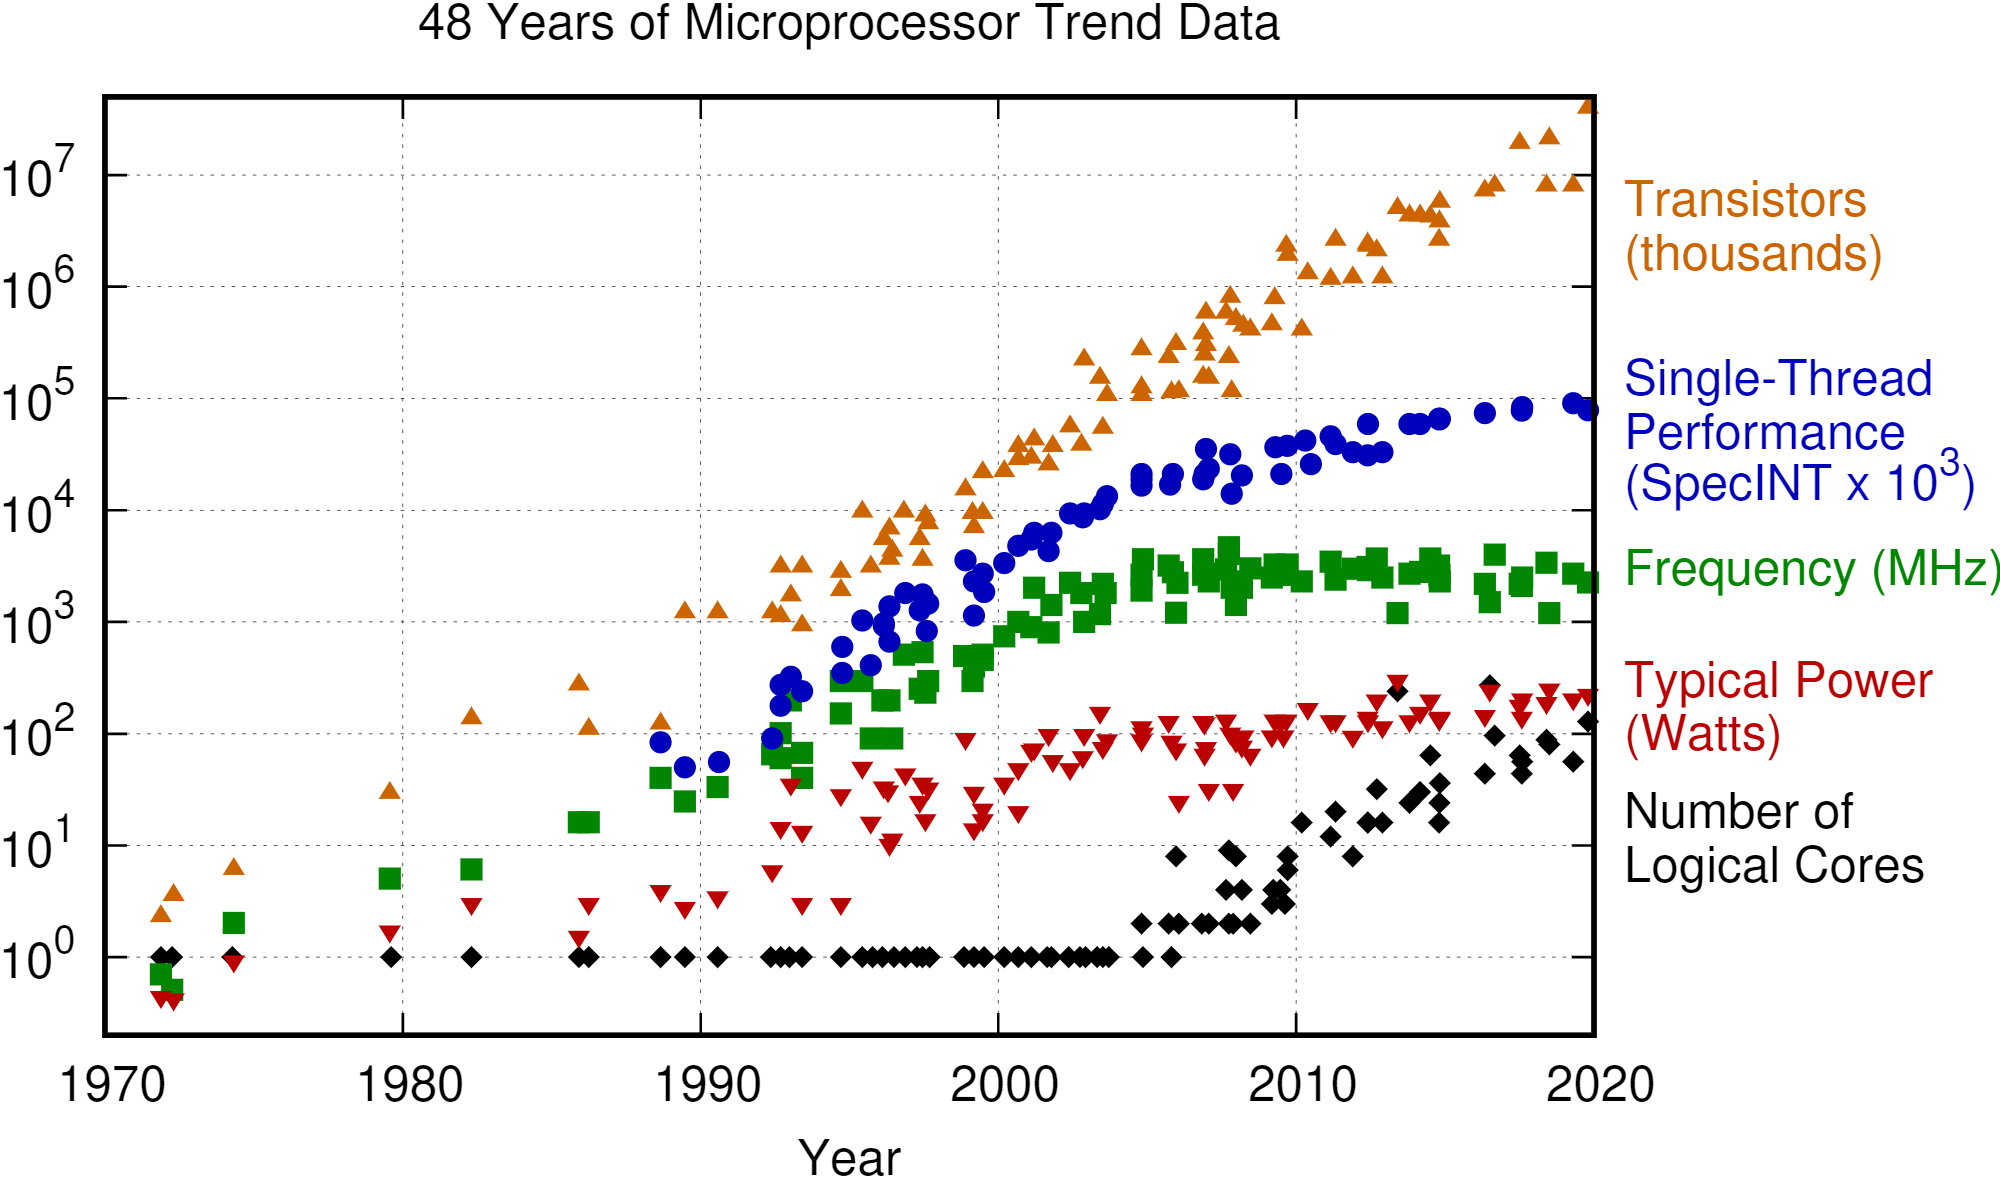
\includegraphics[width=0.95\columnwidth]{gfx/imgs/chapter1/CPUEvolution.png}
    \caption{Evoluzione delle CPU negli ultimi decenni~\cite{repo:cpu-evolution-data}. Nel grafico possiamo notare come la velocità dei transistor (verde) sia rimasta praticamente la stessa negli ultimi 20 anni, mentre il numero di core (nero) abbia continuato ad aumentare in modo pressoché uniforme.}
    \label{fig:cpu-evolution}
\end{figure}

Dunque, il limite principale per la maggior parte dei giochi e delle applicazioni è, e probabilmente sarà almeno per qualche anno, l'utilizzo ottimizzato delle risorse e l'accesso alla memoria. In particolare, ci serve l'impegno del programmatore per strutturare il codice in modo efficiente (ad esempio sfruttando design pattern e design principle) al fine di evitare cache misses e bottleneck. Per approfondire questi argomenti si può fare riferimento a~\cite{article:drepper2007every}.

\subsection{Unity}
Il game engine di \emph{Unity Technologies} è costruito sul component-based model e il suo core è scritto nei linguaggi di programmazione C e C\texttt{++}. Per quanto riguarda lo sviluppo di giochi basati su questo motore, agli sviluppatori finali vengono fornite diverse librerie scritte in linguaggio \Csh. Tali librerie funzionano da wrapper esterno del core del motore di gioco Unity, e sono utilizzate per la scrittura della logica di gioco. In particolare, l'architettura di Unity si basa su due classi fondamentali: 

\begin{enumerate}
    \item \emph{GameObject}. Rappresenta le entità, ovvero gli oggetti presenti nella scena (il mondo/livello in cui esistono)~\cite{doc:unity-gameobjects}.
    \item \emph{MonoBehaviour}. I componenti che realizzano il comportamento delle entità. Solitamente l'implementazione del comportamento avviene tramite il metodo \verb|Update()|, il quale a runtime viene chiamato ad ogni frame~\cite{doc:unity-monobehaviour}.
\end{enumerate}

Il problema principale è l'utilizzo delle risorse, di conseguenza un'architettura di questo genere è perfetta per lo sviluppo di giochi Indie\footnote{Indie è l'abbreviazione del termine inglese \emph{independent} che, in questo caso, fa riferimento ai giochi sviluppati da un singolo programmatore o poche persone, non facenti parte di una software house.}, ma assolutamente inadatta allo sviluppo di applicazioni complesse.

\paragraph{Limiti dell'architettura classica di Unity}
Con \emph{architettura classica} intendiamo il modo tradizionale di sviluppo delle applicazioni su Unity, ovvero tramite la creazione di GameObject o Prefab e l'inserimento di questi in una scena, allegandoci dei MonoBehaviour per fargli fare qualcosa. I MonoBehaviour sono script che ereditano dalla classe \verb|MonoBehaviour|. Il limite di questa soluzione è che introduce un forte legame tra i dati ed il loro processamento (tutto si trova nella stessa classe all'interno del medesimo script). Inoltre, in questo modo abbiamo una stretta dipendenza dai tipi riferimento, i quali gravano molto sulle performance, in quanto indirizzano dei dati che sono sparpagliati in memoria.

Un GameObject è un container che contiene diversi riferimenti ad altre aree di memoria, le quali potrebbero avere altri riferimenti e così via. Quando la CPU deve lavorare su un GameObject, se questo non è presente in cache dev'essere spostato in quest'ultima. Ma poiché è un tipo riferimento, l'operazione può diventare complessa e richiedere molto tempo. Inoltre, spesso ci si trova a processare più dati di quanti effettivamente ne servano.
Ad esempio, i GameObject in Unity devono necessariamente avere un componente \verb|Transform| allegato, che ne specifica la posizione, la rotazione e le dimensioni~\cite{doc:unity-transforms}. Però, matematicamente parlando, se volessimo semplicemente traslare un oggetto, tutto ciò che ci serve è la posizione attuale, la direzione e la velocità di movimento. Nel componente \verb|Transform| (Figura~\ref{fig:transform-class}) ci sono tantissimi altri dati superflui. Tuttavia, quando dobbiamo utilizzare un campo che si trova nel componente Transform, la CPU deve caricarlo tutto in memoria centrale, anche se ce ne serve solo una piccola parte. In questo modo sprechiamo tutto il potenziale delle cache più veloci che, avendo poca memoria, vengono riempite di dati inutili. Inoltre, con l'approccio classico non operiamo veramente su più di un thread. Tutto il processamento dei dati eseguito dai MonoBehaviour avviene in sequenza sul main thread (Figura~\ref{fig:traditional-data-processing}).

\SaveVerb{TransformTerm}|Transform|
\SaveVerb{UnityUnityEngineTerm}|Unity.UnityEngine|

\begin{figure}[!ht]
    \centering
    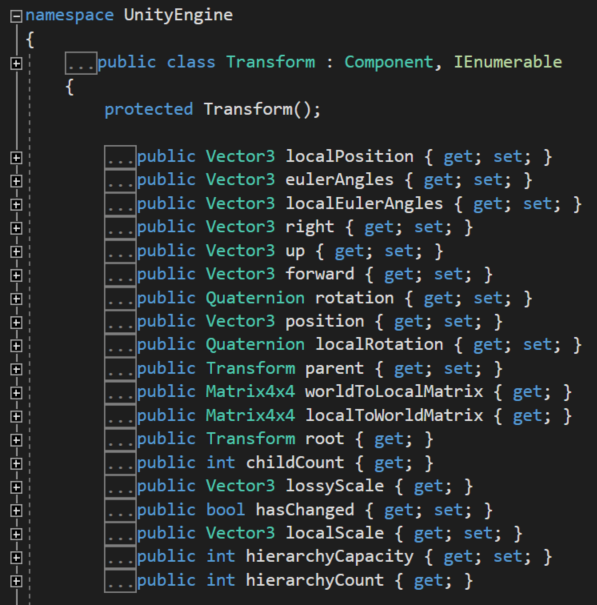
\includegraphics[width=0.64\columnwidth]{gfx/imgs/chapter1/TransformClassUnityEngine.png}
    \caption{Parte della classe \protect \UseVerb{TransformTerm} di \protect \UseVerb{UnityUnityEngineTerm}.}
    \label{fig:transform-class}
\end{figure}

\begin{figure}[!ht]
    \centering
    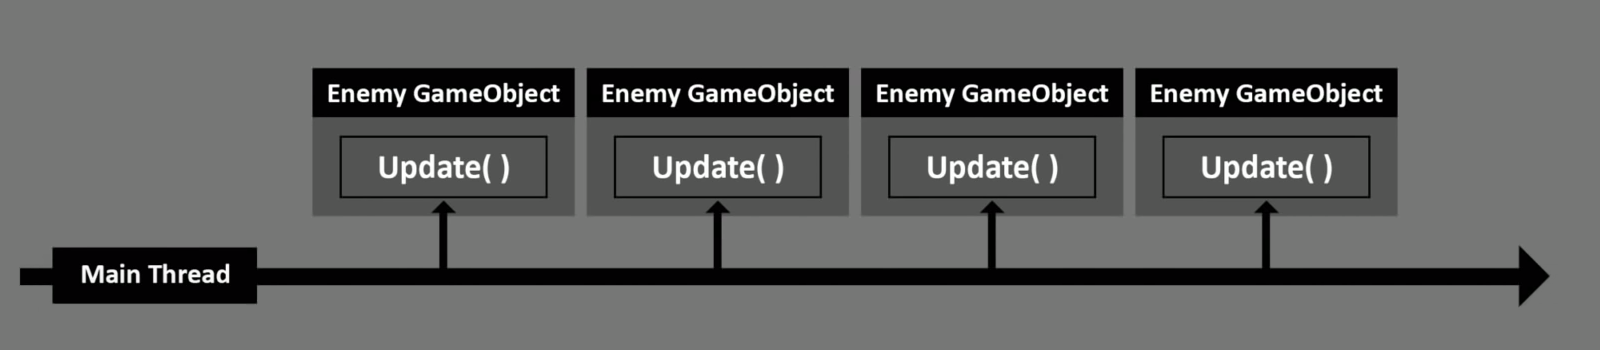
\includegraphics[width=0.90\columnwidth]{gfx/imgs/chapter1/MainThread.png}
    \caption{Processamento dei dati nel modello classico~\cite{youtube:differenze-unity-classico}.}
    \label{fig:traditional-data-processing}
\end{figure}

\subsection{Unreal Engine}
Come Unity, anche il game engine di \emph{Epic Games} è costruito sul component-based model ma, a differenza del primo, Unreal utilizza gli Actor al posto dei GameObject. Possiamo vedere gli Actor come interi oggetti o entità, che possiamo piazzare all'interno del livello di un mondo e possono avere dei componenti che realizzano il comportamento. Sia attori che componenti vengono aggiornati ogni frame tramite un'operazione chiamata \emph{ticking} (in contrapposizione al metodo \verb|Update()| in Unity), che permette di specificare se dev'essere attivata ad ogni frame oppure no~\cite{doc:unreal-architecture}.
Rispetto a Unity, Unreal ottimizza il component-based model, il quale risulta comunque limitato se comparato al modello basato su entità, di cui parleremo nella prossima sezione.

\subsection{Entity Component System}
Entity Component System (ECS) è un pattern architetturale di sviluppo del software che ha come obbiettivo la separazione dei dati dalla logica. Segue il principio del \emph{Composition over Inheritance}, secondo cui le classi dovrebbero realizzare il polimorfismo e il riutilizzo di codice tramite la composizione (contenendo riferimenti), piuttosto che ereditando da una classe padre. Questo ci permette appunto di ottenere maggiore separazione delle competenze e rende il codice flessibile, modulare e, di conseguenza, facilmente leggibile e riutilizzabile~\cite{article:composition-over-inheritance}. Inoltre, eliminando l'overhead generato dalle catene di ereditarietà e tramite l'utilizzo di un approccio data-oriented, ECS permette di raggiungere livelli molto elevati di prestazioni (fondamentali in un videogioco), massimizzando l'utilizzo delle risorse. Infatti, i componenti sono più leggeri e facili da memorizzare degli oggetti: per questo motivo possono essere memorizzati in aree di memoria continue (array) permettendoci di sfruttare al meglio le cache dei processori, in particolare quelle di primo e secondo livello, che sono le più veloci.

Come indica la sigla, ECS comprende tre principali concetti:
\begin{itemize}
    \item \textbf{Entities}. Le ``entità'' che popolano il gioco, che rappresentano un oggetto concreto nell'applicazione. Non contengono né dati né logica, ma sono composte da componenti piccoli, riusabili e generici.
    \item \textbf{Components}. I dati associati alle entità. I componenti immagazzinano i dati o lo stato, ma non contengono alcun tipo di logica. Ciò che caratterizza ECS e lo rende efficiente è il fatto che i componenti sono organizzati proprio per dati e non per entità.
    \item \textbf{Systems}. Realizzano il comportamento. I sistemi contengono la logica che modifica lo stato dei componenti. Ad esempio potremmo creare un sistema che ruota tutte le entità che hanno un componente ``RotateComponent''.
\end{itemize}


\section{Unity DOTS}
Per risolvere i problemi di performance legati al modello su cui si fondava il motore di gioco, nel 2018, Unity ha presentato una soluzione basata su un design orientato ai dati~\cite{book:data-oriented-design}: DOTS.

\emph{Data-Oriented Technology Stack} (DOTS) è un insieme di librerie realizzate dagli sviluppatori di Unity negli ultimi due anni, tutt'oggi in fase di sviluppo. Il loro scopo fu quello di rivoluzionare l'architettura del game engine facendo in modo che le prestazioni non venissero limitate dal modello su cui si basava. A tal proposito, nello stack sono stati inseriti diversi package, fra cui in particolare ECS e Job System, che permettono di risolvere i principali problemi della vecchia architettura, e NetCode, per rivoluzionare il modello networking.

Il Job System permette di sfruttare il multi-core processing tramite il multithreading, così da non caricare tutto il lavoro su uno o due core, ma distribuirlo uniformemente, sfruttando il più possibile anche gli altri core della CPU. Inoltre, il Job System gestisce da solo tutti i problemi legati al multithreading (scrivere codice thread-safe è difficile, dobbiamo evitare corse critiche, il context switching è costoso, ecc.), così che lo sviluppatore possa focalizzarsi sulla logica o altri aspetti del gioco.

ECS permette di organizzare meglio il codice separando i dati dalle funzionalità, garantendo diversi benefici:
\begin{itemize}
    \item Scrivere codice non performante con DOTS diventa difficile, proprio grazie al modello ECS su cui si basa, il quale è performante a propri (\emph{performance by default}).
    \item È facile scrivere codice altamente ottimizzabile e riutilizzabile.
    \item Permette di sfruttare al meglio l'architettura hardware su cui il codice esegue, in quanto i dati sono memorizzati per archetipo, in modo molto compatto ed efficiente. Come conseguenza, tutte le operazioni che esegue la CPU sui dati (fetching, caricamento, ecc.) sono velocizzate, massimizzando l'utilizzo delle risorse e riducendo i consumi~\cite{youtube:overview-ecs-job}.
\end{itemize}

\SaveVerb{RotationTerm}|Rotation|
\SaveVerb{TranslationTerm}|Translation|
\SaveVerb{LocalToWorldTerm}|LocalToWorld|

\begin{figure}[!ht]
    \centering
    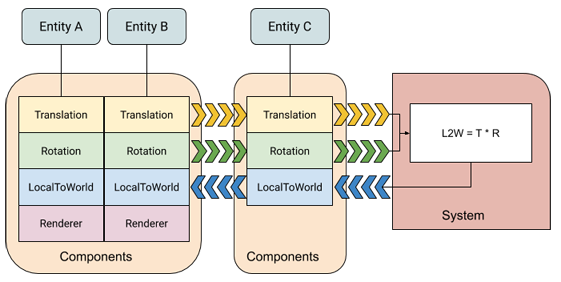
\includegraphics[width=0.90\columnwidth]{gfx/imgs/chapter1/ECSBlockDiagram.png}
    \caption{Esempio di funzionamento del pattern ECS: il sistema sulla destra prende in ingresso i componenti \UseVerb{TranslationTerm} e \UseVerb{RotationTerm} delle entità e aggiorna \UseVerb{LocalToWorldTerm} con il loro prodotto~\cite{doc:unity-entities-manual}.}
    \label{fig:ecs-example}
\end{figure}
Infine, NetCode fornisce un modello di networking a server autoritativo con server dedicato e predizione del client. Questo permette di ridurre al minimo la latenza, migliorando notevolmente l'esperienza di gioco. Di conseguenza, si presta molto bene ad essere utilizzato per la realizzazione di giochi che richiedono requisiti di lag minimi, quali ad esempio gli FPS.

Il resto della tesi è organizzato come segue.

\paragraph{Capitolo 2}
Introdurremo il package Entities, illustrando le API ed i costrutti fondamentali, spiegando com'è possibile realizzare il modello a Entity Component System in Unity. Inoltre, forniremo degli esempi, e spiegheremo le differenze sostanziali con l'architettura classica basata su GameObject e MonoBehaviour.

\paragraph{Capitolo 3}
Apriremo questo capitolo fornendo un background sulla realizzazione di videogiochi multiplayer, mostrando le principali topologie di rete, i protocolli utilizzati ed i problemi che si possono riscontrare. Dopodiché tratteremo il package Transport, che si occupa di sostituire le vecchie API di basso livello di UNet, ed infine il package NetCode, che assumerà particolare rilevanza soprattutto per il capitolo successivo.

\paragraph{Capitolo 4}
In questo capitolo mostreremo le funzionalità ed i passaggi utilizzati per realizzare il prototipo basato su DOTS. In particolare spiegheremo il significato e la funzione dei principali file implementati per il progetto.

\paragraph{Capitolo 5}
Effettueremo un'analisi qualitativa del prototipo realizzato e introdurremo un secondo prototipo, molto più semplice, che ci tornerà utile ai fini di testing e valutazione delle performance. Per farlo vedremo come utilizzare il Profiler Unity per ricavare informazioni riguardanti le prestazioni. 

\paragraph{Conclusioni e Sviluppi Futuri}
In questo capitolo trarremo le conclusioni, analizzando soprattutto i risultati ottenuti nel capitolo precedente e proponendo dei possibili sviluppi futuri.       % 1.Evoluzione Game Engine
\cleardoublepage

\chapter{Unity DOTS: Entity Component System}
\label{cap:ecs}
% NB: le parole al plurale in inglese vengono declinate al singolare in italiano, anche se la frase è al plurale

Per Unity, ECS è il nucleo della nuova tecnologia DOTS, in quanto è ciò che permette di realizzare il pattern data-oriented. Per utilizzarlo in un progetto dobbiamo importare il package \emph{Entities} (\verb|com.unity.entities|).

% esempio: come introdotto nella sezione ref... (citare)

%%%%%%%%%%%%%%%%%%%%%%%%%%%%%%%%%%%%%%%%%%%%%%%%%%%%%%%%%%%%%%%%%%%%%%%%%%%%%
\section{Introduzione a ECS}

Un'architettura di tipo ECS separa i tre concetti di entità, stato e comportamento, e si concentra sui dati di basso livello. I sistemi leggono stream di dati dei componenti, quindi li trasformano da dati di input a dati di output, e le entità indicizzano questi ultimi.

\paragraph{Archetipi}

Un \emph{EntityArchetype} è una combinazione unica di certi tipi di componenti. Ogni entità ne ha uno e quando vengono aggiunti o rimossi componenti all'entità, il suo archetipo cambia (esempio in Figura~\ref{fig:archetype}).

\begin{figure}[!ht]
    \centering
    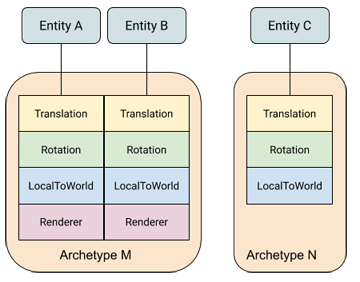
\includegraphics[width=0.60\columnwidth]{gfx/imgs/chapter2/ArchetypeDiagram.png}
    \caption{Esempi di archetipi: le entità A e B hanno lo stesso archetipo in quanto possiedono lo stesso set di componenti~\cite{doc:unity-entities-manual}.}
    \label{fig:archetype}
\end{figure}

\paragraph{Chunk di memoria}
L'archetipo di una entità determina dove i componenti di questa vengono memorizzati. ECS alloca memoria in blocchi chiamati \emph{ArchetypeChunk}, ognuno dei quali è rappresentato da un archetipo e contiene sempre e solo entità di quello stesso archetipo (Figura~\ref{fig:memory-chunk}). I chunk sono costituiti da array di componenti e, quando l'archetipo di un'entità cambia (ad esempio vengono aggiunti o rimossi componenti), questa viene spostata in un chunk differente.

\begin{figure}[!ht]
    \centering
    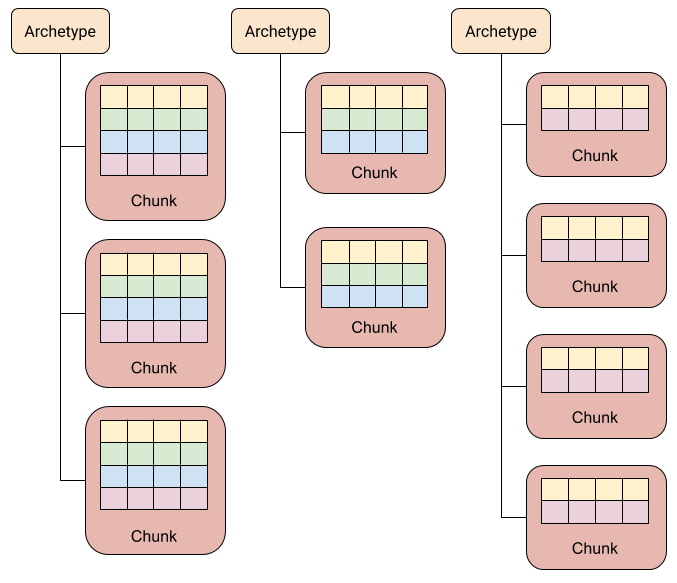
\includegraphics[width=0.85\columnwidth]{gfx/imgs/chapter2/ArchetypeChunkDiagramENG.png}
    \caption{Organizzazione delle entità nei chunk di memoria~\cite{doc:unity-entities-manual}.}
    \label{fig:memory-chunk}
\end{figure}

\paragraph{EntityQuery}

Quando realizziamo del comportamento, dobbiamo individuare quali entità il sistema deve processare. Per farlo utilizziamo, direttamente o indirettamente, una \emph{EntityQuery}. Questa non è altro che una descrizione delle entità su cui vogliamo iterare. Infatti, permette di cercare gli archetipi esistenti per le entità che hanno i componenti corrispondenti a quelli indicati, fornendo una lista dei chunk su cui possiamo iterare.

\paragraph{Jobs}

Il \emph{\Csh{} Job System} di Unity permette di sfruttare i vantaggi del multithreading per eseguire del comportamento in parallelo. A tal proposito ECS fornisce dei meccanismi (ad esempio, \verb|Entities.ForEach| di \verb|SystemBase|) che permettono di eseguire operazioni al di fuori del main thread. I job vengono schedulati in base alle dipendenze che hanno fra di loro e all'ordine in cui i sistemi sono organizzati.

Poiché ECS introduce tipi e costrutti nuovi, DOTS fornisce il package \emph{Jobs}, che estende le funzionalità del \Csh{} Job System di Unity con tipi utili e compatibili con le entità~\cite{doc:unity-jobs}.

\paragraph{Organizzazione dei sistemi}

I sistemi in ECS sono organizzati per \emph{world} e \emph{group}. Di base viene creato un mondo predefinito chiamato DefaultWorld, con un insieme prefissato di gruppi e sistemi. Quindi ECS trova tutti i sistemi (gli script del proprio progetto), li istanzia e li aggiunge al gruppo SimulationGroup nel DefaultWorld, se non specificato in modo differente. I sistemi vengono aggiornati, ovvero viene invocato il metodo \verb|OnUpdate()|, nell'ordine in cui sono posizionati all'interno del gruppo a cui appartengono, a meno che non lo specifichiamo manualmente.

\paragraph{Authoring data e runtime data}

Esistono due fondamentali tipi di dati in Unity: \emph{authoring data} e \emph{runtime data}. Gli authoring data sono tutti quei tipi ed oggetti che riguardano la creazione nell'editor, ad esempio i GameObject presenti nella scena. Questi sono ottimizzati per essere flessibili (facilmente leggibili e modificabili, infatti Unity fornisce il pannello \emph{Inspector} per accederli). Inoltre, negli authoring data esistono gerarchie, ogni oggetto ha un nome e ci sono diverse informazioni di cui non si ha veramente bisogno a runtime; i runtime data, invece, sono i dati a tempo di esecuzione in \emph{Play Mode}\footnote{Edit Mode e Play Mode sono le due modalità in cui possiamo eseguire Unity. In particolare, per entrare in play mode è possibile utilizzare l'apposito pulsante nell'editor, oppure lanciare un'applicazione standalone.}, ad esempio le entità ed i componenti. In particolare, i runtime data sono ottimizzati per le performance (efficienza delle cache, tempi di caricamento e streaming, dimensioni di distribuzione).

Unity DOTS dispone di un conversion workflow che ci permette di convertire i GameObject in entità, e questa conversione avviene nell'editor.

%%%%%%%%%%%%%%%%%%%%%%%%%%%%%%%%%%%%%%%%%%%%%%%%%%%%%%%%%%%%%%%%%%%%%%%%%%%%%
% Pagine API: ArchetypeChunk, Entity, EntityManager, IJobEntityBatch, EntityQuery, World, WorldFlags
\section{Entities}

Le entità rappresentano le ``cose'' individuali del nostro gioco/applicazione. Non contengono né dati né comportamento, piuttosto definiscono quali parti di dati dovrebbero stare insieme. Le entità sono essenzialmente il rimpiazzo dei GameObject ma, mentre questi ultimi non sono altro che dei contenitori, le entità rappresentano degli indici. Infatti, mentre i GameObject sono delle classi, le entità sono semplici strutture, che contengono solo un ID ed un numero di versione per verificare se l'ID è ancora valido. Per avere un più chiaro esempio, una entità è paragonabile alla chiave di una tupla di un database.

Il fatto che sia entità che componenti siano implementati tramite delle strutture è un aspetto molto significativo. Le strutture sono infatti il modo più efficiente di immagazzinare dati per CPU e memoria; e sono estremamente sicure dal punto di vista del multithreading e del typing~\cite{article:ecs-data-structures}.

Solitamente non utilizziamo mai direttamente l'ID o il numero di versione di una entità per accedervi, ma passiamo la struttura a dei metodi. A tal proposito esiste una struttura, chiamata \verb|EntityManager|, che gestisce tutte le entità di un world. Essa mantiene una lista delle entità ed organizza i dati associativi per ottenere performance migliori. L'\verb|EntityManager| contiene tutte le API per: creare, leggere, aggiornare e distruggere le entità. Ogni \verb|World| possiede un unico \verb|EntityManager|, il quale gestisce tutte le entità presenti nel mondo a cui esso è associato~\cite{doc:unity-entities-api}.

\subsection{Creazione delle entità}

Esistono diversi modi per creare le entità. Il più semplice ed utilizzato è quello che sfrutta il \emph{Conversion Workflow} di DOTS. Questo permette di convertire i GameObject ed i prefab presenti nell'editor in entità, semplicemente inserendoli all'interno di una subscene\footnote{Le SubScene di DOTS permettono di convertire in entità tutti i GameObject che contengono. Quando chiudiamo una subscene, viene scritta una copia binaria delle entità memorizzate in cache, che permette di velocizzare il caricamento della subscene a runtime. Così facendo l'applicazione diventa notevolmente scalabile.}. Un secondo metodo consiste nell'utilizzo dell'\verb|EntityManager|, che espone la funzione \verb|CreateEntity()| per:

\begin{itemize}
    \item Creare entità dato un array di \verb|ComponentType| o un \verb|EntityArchetype|.
    \item Copiare un'entità già esistente.
    \item Creare un'entità senza componenti. 
\end{itemize}

Le entità create in questo modo vengono aggiunte al \verb|World| in cui si trova l'\verb|EntityManager|~\cite{doc:unity-entities-api}.
   
\begin{figure}[!ht]
    \centering
    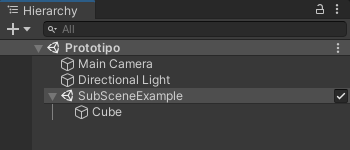
\includegraphics[width=0.70\columnwidth]{gfx/imgs/chapter2/SubSceneConversionWorkflow.png}
    \caption{Esempio di conversione di un GameObject ``Cube'' nella rispettiva entità, tramite subscene.}
    \label{fig:subscene-example}
\end{figure}

\subsubsection{Aggiunta e rimozione dei componenti}

Una volta creata una entità, possiamo aggiungervi o rimuoverne dei componenti utilizzando i metodi dell'\verb|EntityManager|. Quando ciò avviene l'archetipo dell'entità cambia ed ECS muove i dati in un nuovo chunk.

Le modifiche ad un'entità che causano cambiamenti strutturali (creazione$/$rimozione entità, aggiunta$/$rimozione di componenti e cambiamenti al valore di componenti condivisi) non sono operazioni thread-safe, quindi non possono essere effettuate all'interno di un job. Per eseguirle dobbiamo aggiungerle ad una struttura \verb|EntityCommandBuffer| ed applicarle una volta terminato il job~\cite{doc:unity-entities-api}.

\subsection{Accedere ai dati di un'entità}
In ECS, il modo più comune per accedere ai dati delle entità (ovvero al contenuto dei componenti) all'interno dei sistemi, è quello dell'iterazione. Tipicamente i sistemi ECS processano un set di entità, leggendo i dati da uno o più componenti, effettuando dei calcoli e scrivendo i risultati su altri componenti.
Il \Csh{} Job System permette di utilizzare i job per processare i componenti in parallelo, al fine di sfruttare al massimo la potenza di calcolo di tutti i core del processore e la località dei dati, evitando i cache misses.
ECS fornisce diverse API per realizzare l'iterazione, in particolare \verb|Entities.ForEach| all'interno di una classe \verb|SystemBase| (la classe per realizzare i sistemi), permette di utilizzare un \emph{lambda expression} per iterare su tutte le entità con un certo set di componenti.

La documentazione del package Entities sconsiglia di utilizzare alcuni costrutti, in quanto sono obsoleti e verranno deprecati in futuro~\cite{doc:unity-entities-manual}:
\begin{itemize}
    \item \verb|IJobChunk|.
    \item \verb|IJobForEach|.
    \item \verb|IJobForEachWithEntity|.
    \item \verb|ComponentSystem|.
    \item \verb|JobComponentSystem|.
\end{itemize}

\subsection{World}
Un \emph{world} organizza le entità, che esistono e hanno significato solo per il mondo in cui si trovano, in gruppi isolati. Esso possiede sia un \verb|EntityManager| che un set di sistemi, i quali possono accedere solo alle entità nel mondo di cui fanno parte.

Quando l'applicazione viene messa in esecuzione (o si entra in Play Mode) Unity crea un mondo di default chiamato DefaultWorld. Dopodiché istanzia tutti i sistemi (ovvero le classi che ereditano da \verb|ComponentSystemBase|, fra cui \verb|SystemBase|) e li aggiunge a tale mondo ~\cite{doc:unity-entities-manual}.

\paragraph{Gestione dei sistemi}
Uno dei compiti del mondo è quello di gestire i sistemi che vi fanno parte. Inoltre, la classe \verb|World| fornisce metodi per la creazione, l'accesso e la rimozione dei sistemi~\cite{doc:unity-entities-api}.

\paragraph{Tempo}
L'oggetto \verb|World| gestisce e controlla anche la proprietà \verb|Time| dei sistemi che vi fanno parte. Questa proprietà può essere utilizzata per ottenere il tempo nel mondo corrente e spesso è utile per definire comportamenti che utilizzano variabili dipendenti dal tempo (ad esempio la velocità).

\SaveVerb{TimeTerm}|Time|

\begin{lstlisting}[caption={Prototipo: utilizzo della proprietà \UseVerb{TimeTerm} per ruotare delle entità.},label={lst:time-property-example},language={[Sharp]C}]
public class RotateCollectibleSystem : SystemBase
{
    protected override void OnUpdate()
    {
        float deltaTime = Time.DeltaTime; // ottiene il tempo attuale

        Entities.ForEach((ref Rotation rotation, in RotationSpeedComponent rsc) =>
        {
            rotation.Value = math.mul(rotation.Value, quaternion.RotateX(math.radians(rsc.X * deltaTime)));
            rotation.Value = math.mul(rotation.Value, quaternion.RotateY(math.radians(rsc.Y * deltaTime)));
            rotation.Value = math.mul(rotation.Value, quaternion.RotateZ(math.radians(rsc.Z * deltaTime)));
        }).Run();
    }
}
\end{lstlisting}

Di default Unity crea una struttura \verb|TimeData| per ogni world. A tempo di esecuzione questa viene convertita in un'entità \verb|WorldTime|, che possiede un componente \verb|DeltaTime|. Quest'ultimo viene aggiornato continuamente dal sistema \verb|UpdateWorldTimeSystem| per rispecchiare il tempo passato rispetto al frame precedente. La proprietà \verb|Time| di un sistema è semplicemente un alias per l'entità \verb|WorldTime|.

\SaveVerb{WorldTimeTerm}|WorldTime|
\SaveVerb{DeltaTimeTerm}|DeltaTime|

\begin{figure}[!ht]
    \centering
    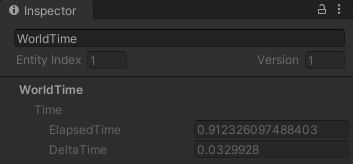
\includegraphics[width=0.65\columnwidth]{gfx/imgs/chapter2/WorldTimeEntity.png}
    \caption{Entità \UseVerb{WorldTimeTerm} ed il suo componente \UseVerb{DeltaTimeTerm} a runtime.}
    \label{fig:worldtime-entity}
\end{figure}

%%%%%%%%%%%%%%%%%%%%%%%%%%%%%%%%%%%%%%%%%%%%%%%%%%%%%%%%%%%%%%%%%%%%%%%%%%%%%
\section{Components}
I componenti rappresentano i dati del nostro gioco/applicazione, citando Maxim Zaks in ~\cite{article:components-definition}, essi sono «le parti atomiche dei nostri dati». In Unity ECS un componente è separato dal comportamento ed possiamo realizzarlo tramite una struttura che implementa una delle seguenti interfacce:
\begin{itemize}
    \item \verb|IComponentData|. È la più utilizzata e permette di definire un componente generico.
    \item \verb|IBufferElementData|. Permette di definire un componente contenente un buffer dinamico.
    \item \verb|ISharedComponentData|. Permette di definire un componente il cui valore viene condiviso da tutte le entità nello stesso chunk (ECS organizza o raggruppa le entità in base al valore di questo, all'interno di un archetipo);
    \item Componenti ibridi. Permettono di aggiungere i componenti di UnityEngine (GameObject) alle entità. Il principale motivo della loro esistenza è che DOTS è ancora in fase di sviluppo e molte feature di Unity ancora non hanno il corrispondente in ECS.
    \item \verb|ISystemStateComponentData|. Permettono di associare uno stato specifico di un sistema ad un'entità, rilevando quando le singole entità vengono create o distrutte.
    \item \verb|ISharedSystemStateComponentData|. Combina gli shared component ed i system state component.
    % RICONTROLLARE - blob footnote?
    \item \verb|BlobAsset|. Non è un vero e proprio componente ma possiamo utilizzarlo per memorizzare dati. Un blob (Binary Large OBject) asset è una struttura immutabile immagazzinata in memoria \emph{unmanaged} (ovvero per la quale non esiste un Garbage Collector che la pulisca), che può essere referenziato da uno o più componenti tramite \verb|BlobAssetReference|. Solitamente li usiamo per condividere dati fra asset e potervi accedere nei \Csh{} Job.
\end{itemize}

L'\verb|EntityManager| organizza combinazioni uniche di componenti tramite gli archetipi e memorizza i componenti di tutte le entità con lo stesso archetipo negli stessi chunk di memoria (tutte le entità in uno stesso chunk di memoria hanno tutte lo stesso archetipo)~\cite{doc:unity-entities-manual}.

I componenti di maggior interesse ai fini della tesi e dello sviluppo del prototipo sono \verb|IComponentData| e \verb|BufferElementData|. A tal proposito non tratteremo nel dettaglio gli altri, per i quali rimandiamo alla documentazione ufficiale~\cite{doc:unity-entities-manual}.

\subsection{Componenti generici}
Un componente generico è una struttura (quindi di default viene copiato per valore) che implementa l'interfaccia \verb|IComponentData|, fornita dal package Entities. Essendo una struttura, il componente può contenere solo tipi unmanaged e blittable, ovvero quei tipi di dato che vengono rappresentati nello stesso modo sia in memoria managed che unmanaged e non richiedono una gestione particolare da parte del marshaler di interoperabilità~\cite{doc:microsoft-blittable-types}.

Una singola implementazione di un componente dovrebbe contenere solo campi per dati che vengono acceduti sempre, o quasi, allo stesso tempo. Infatti, solitamente, avere un maggior numero di componenti piccoli è più efficiente rispetto all'avere pochi componenti ma grossi. Questo a causa del \emph{memory alignment} delle strutture: la CPU, per motivi di performance, memorizza i campi di una struttura sequenzialmente nell'ordine in cui sono dichiarati (il primo ha l'indirizzo di memoria più basso, l'ultimo il più alto). Ogni tipo di dato ha il proprio requisito di allineamento e, per le strutture, il requisito è il campo con la dimensione maggiore. Di conseguenza, se i campi sono di dimensioni diverse, solitamente la memoria totale allocata per la struttura è maggiore di quella minima che servirebbe, in quanto vengono inseriti degli offset per allineare i dati~\cite{doc:microsoft-memory-alignment}.

\verb|IComponentData| può anche essere implementato come classe, ad esempio per il porting in ECS di codice già esistente, ma ciò presenta numerosi svantaggi, ad esempio non può usufruire del Burst compiler (Sezione~\ref{subsubsec:impl-sistema}).

\begin{lstlisting}[caption={Prototipo: esempio di componente generico.},label={lst:generic-component-example},language={[Sharp]C}]
[GenerateAuthoringComponent]
public struct PlayerMovementSpeed : IComponentData
{
    public float speed;
}
\end{lstlisting}

\subsection{Aggiunta e rimozione dei componenti da un'entità}
L'\verb|EntityManager| espone metodi per aggiungere e rimuovere dei componenti da un'entità, e metodi per leggerne e impostarne il valore. Un'alternativa, è quella di utilizzare un \verb|EntityCommandBuffer|, una struttura thread-safe che permette di bufferizzare dei comandi (che agiscono anche su entità e componenti) per eseguirli più tardi, ma tutti in una volta nel frame.
Oltre a questi due metodi, ne esiste un terzo: aggiungendo l'attributo \verb|[GenerateAuthoringComponent]| alla struttura che implementa il componente, possiamo allegare il componente ad un GameObject presente nella scena. Così facendo, quando il GameObject verrà convertito in entità dal sistema di conversione, gli verrà assegnato tale componente.

\subsection{Accedere ai componenti di un'entità}
Solitamente l'accesso ai componenti viene fatto all'interno di un sistema, il quale itera su tutte le entità filtrate da una query che specifica un particolare set di componenti. Ad esempio, la query potrebbe specificare che devono essere filtrate solo le entità che hanno un componente \verb|PlayerMovementSpeed|, così che il sistema \verb|PlayerMovementSystem| possa implementare il movimento del giocatore e muovere solo l'entità del player.

\subsection{Buffer dinamici}
Un buffer dinamico è un particolare tipo di componente ECS che associa dei dati sotto forma di array ad una entità. È dinamico in quanto può contenere un numero variabile di elementi, ridimensionandosi automaticamente quando necessario. Possiamo anche specificarne una dimensione interna, tramite l'attributo \verb|[InternalBufferCapacity]|, che indica il numero di elementi che il buffer memorizza nell'ArchetypeChunk relativo. In tal caso, se il numero di elementi dovesse eccedere, il buffer allocherebbe un blocco di memoria heap (gestita completamente da ECS) fuori dal chunk, spostandovi tutti gli elementi~\cite{doc:unity-entities-manual}.

Per creare un buffer dinamico dobbiamo creare una struttura che implementa \verb|IBufferElementData|, definendo al suo interno il tipo di elemento che il buffer dovrà contenere.

\begin{lstlisting}[caption={Esempio buffer dinamico.},label={lst:dynamic-buffer},language={[Sharp]C}]
public struct IntBufferElement : IBufferElementData
{
    public int Value;
}
\end{lstlisting}

Per aggiungere il buffer ad un'entità, vi aggiungiamo semplicemente la struttura che implementa \verb|IBufferElementData|, come per un normale componente generico. \verb|EntityManager| e \verb|EntityCommandBuffer| espongono funzioni che permettono di aggiungere il buffer ad un'entità, restituendo una struttura container \verb|DynamicBuffer<T>|. Questa ci permette di accedere agli elementi \verb|inIBufferElementData| tramite un'interfaccia più ``array-like''.
Inoltre, \verb|DynamicBuffer<T>| fornisce un metodo \verb|Reinterpret<T>| che permette di reinterpretare il buffer con uno i cui elementi abbiano un tipo diverso, ma delle stesse dimensioni in memoria. Ciò permette di ottenere un handle sicuro per il buffer originale, utilizzando un riferimento, così che le modifiche siano correlate. Lo scopo è semplificare l'utilizzo del buffer, in quanto creare una struttura ogni volta per inserire un elemento può essere molto dispendioso e soggetto ad errori.

\SaveVerb{ReinterpretTerm}|Reinterpret<T>|

\begin{lstlisting}[caption={Esempio di utilizzo del metodo \UseVerb{ReinterpretTerm}.},label={lst:dynamic-buffer-reinterpret},language={[Sharp]C}]
DynamicBuffer<IntBufferElement> buffer1;
buffer.Add(new IntBufferElement() { value = 1 }); // dispendioso
DynamicBuffer<int> buffer2 = buffer1.Reinterpet<int>();
buffer2.Add(2); // semplice
\end{lstlisting}

%%%%%%%%%%%%%%%%%%%%%%%%%%%%%%%%%%%%%%%%%%%%%%%%%%%%%%%%%%%%%%%%%%%%%%%%%%%%%
\section{Systems}
Un sistema ECS è una classe che implementa il comportamento, fornendo la logica che trasforma i dati memorizzati in un componente dal suo stato corrente ad un altro stato. Un sistema opera su un insieme di entità che hanno un particolare set di componenti, specificato tramite una query, leggendo e scrivendo dati nei componenti di interesse.

\SaveVerb{DeleteTagComponentTerm}|DeleteTagComponent|
\SaveVerb{EntityCommandBufferTerm}|EntityCommandBuffer|

\begin{lstlisting}[caption={Prototipo: sistema che elimina tutte le entità che possiedono il componente \UseVerb{DeleteTagComponentTerm}, utilizzando un \UseVerb{EntityCommandBufferTerm}.},label={lst:system-simple-example},language={[Sharp]C}]
public class DeleteCollectibleSystem : SystemBase
{
    protected override void OnUpdate()
    {
        EntityCommandBuffer commandBuffer = new EntityCommandBuffer(Unity.Collections.Allocator.Temp);

        Entities
            .WithAll<DeleteTagComponent>()
            .ForEach((Entity entity) =>
            {
                commandBuffer.DestroyEntity(entity);
            }).Run();

        commandBuffer.Playback(EntityManager);
        commandBuffer.Dispose();
    }
}
\end{lstlisting}

% o subsub?
\paragraph{Cosa cambia rispetto ai MonoBehaviour classici}
Sia i sistemi che i MonoBehaviour sono classi e contengono metodi per realizzare il comportamento (i MonoBehaviour hanno la funzione \verb|Update()| che viene chiamata ad ogni frame, i sistemi hanno \verb|OnUpdate()|).

In Unity classico, quando vengono chiamate le \verb|Update()| di alcuni GameObject, anche se sono dello stesso tipo, tutte le operazioni vengono fatte sequenzialmente sul main thread. Quest'ultimo, infatti, itera su una lista di GameObject, accedendo al MonoBehaviour di ciascuno e chiamando per ciascuno la \verb|Update()| che realizza il comportamento. Ad esempio, se ci fossero dei GameObject zombie, significa che ognuno di questi muove se stesso per la mappa.
Al contrario, in ECS il sistema è completamente separato dalle entità su cui agisce: nel metodo \verb|OnUpdate()| vengono filtrate le entità con i componenti che vogliamo modificare, dopodiché vengono svolte delle operazioni su tali componenti. Quindi c'è un solo sistema che realizza una funzionalità specifica per tutte le entità coinvolte.

Così facendo si ottiene non solo separazione della logica, ma anche un modo semplice per realizzare le operazioni in parallelo, in quanto il codice dei sistemi può essere facilmente eseguito tramite job parallelizzabili. Inoltre, le operazioni di fetch delle entità su cui lavorare sono estremamente rapide, perché quelle con gli stessi componenti si trovano tutte raggruppate negli stessi chunk~\cite{youtube:differenze-unity-classico}.


\paragraph{Perché i sistemi sono così efficienti}
ECS è stato progettato avendo una chiara idea di come funziona l'hardware su cui il codice esegue.
Se il fetch della CPU avviene su dati che si trovano in cache di primo livello (le più efficienti), questa sarà un'operazione estremamente veloce, quindi sarebbe meglio sfruttarle il più possibile.

Nell'architettura classica, con i GameObject, ogni volta che la CPU caricava una cache line per mettere dei dati in cache, questa veniva riempita per buona parte di dati inutili. Ciò era dovuto al fatto che, anche se di un componente fosse servito solo il valore di un campo, la CPU lo avrebbe caricato comunque tutto nella cache line, compresi i dati superflui (un esempio è il componente Transform, che contiene moltissime dichiarazioni che raramente servono, vedi Figura~\ref{fig:transform-class}).

Al contrario, per com'è strutturato ECS, i componenti si trovano negli archetype chunk, dove i dati sono immagazzinati in array. Allineandosi perfettamente in memoria, possono essere caricati nella cache line con un overhead minimo.
Inoltre, ciò va anche a vantaggio del prefetching: non è difficile predire cosa succederà quando iteriamo su una serie di entità che hanno tutte gli stessi componenti, salvati in memoria in sequenze tutte uguali. Infatti, questo permette alla CPU di riconoscere il pattern e iniziare il fetching di due cache line alla volta. Ciò sarebbe stato impossibile con i GameObject, poiché spesso solo una piccolissima parte della cache line era utile alla CPU, mentre tutto il resto era da buttare~\cite{youtube:differenze-unity-classico}.

\subsection{Creazione di un sistema}
Per creare un sistema in Unity ECS è necessario implementare la classe astratta \verb|SystemBase| ed almeno il metodo di callback \verb|OnUpdate()|. Questo metodo viene chiamato ad ogni frame di esecuzione del gioco e viene attivato dalla \verb|OnUpdate()| del gruppo padre a cui il sistema appartiene.
Tutti gli eventi di un sistema eseguono sul main thread e solitamente all'interno di \verb|OnUpdate()| scheduliamo un job che esegue la maggior parte delle operazioni. Esistono diversi modi per farlo, in particolare:
\begin{itemize}
    \item \verb|Entities.ForEach|. È il modo più semplice ed utilizzato per iterare su componenti ECS.
    \item \verb|Job.WithCode|. Fornisce un meccanismo per implementare dei job singoli che possono eseguire anche in background, tramite una lambda expression.
    \item \verb|IJobEntityBatch|. fornisce un meccanismo di basso livello iterare su un set di istanze di \verb|ArchetypeChunk|, dove ogni istanza rappresenta un gruppo di entità in un chunk.
    \item \Csh{} Job System. permette di creare e schedulare job \Csh{} generici.
\end{itemize}

\subsubsection{Ciclo di vita di un sistema}
La classe \verb|SystemBase| da cui il sistema eredita, a seconda delle esigenze, può implementare le seguenti callback, che vengono chiamate in diversi momenti dell'esecuzione:
\begin{enumerate}
    \item \verb|OnCreate()|. Quando il sistema viene creato.
    \item \verb|OnStartRunning()|. Prima della prima \verb|OnUpdate()| ed ogni volta che il sistema riprende l'esecuzione.
    \item \verb|OnUpdate()|. Ad ogni frame fintanto che il sistema ha del lavoro da svolgere e la proprietà \verb|Enabled| è vera.
    \item \verb|OnStopRunning()|. Ogni volta che il sistema smette di aggiornare, ad esempio perché \verb|Enabled| è falso, oppure quando la query non trova entità corrispondenti al filtro. Viene anche chiamata prima di \verb|OnDestroy()|.
    \item \verb|OnDestroy()|. Quando il sistema viene distrutto.
\end{enumerate}

A meno che non scheduliamo dei job all'interno di \verb|OnUpdate()|, queste funzioni eseguono tutte sul main thread, nell'ordine mostrato in Figura~\ref{fig:system-callbacks}~\cite{doc:unity-entities-api}.

\SaveVerb{SystemBaseTerm}|SystemBase|

\begin{figure}[!ht]
    \centering
    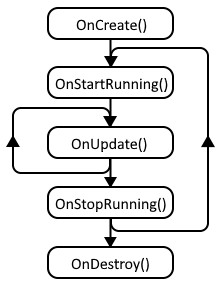
\includegraphics[width=0.34\columnwidth]{gfx/imgs/chapter2/SystemEventCallbacks.png}
    \caption{Callback di \UseVerb{SystemBaseTerm} e ordine in cui vengono chiamate.}
    \label{fig:system-callbacks}
\end{figure}

\subsubsection{Implementazione del comportamento con Entities.ForEach}
\label{subsubsec:impl-sistema}
La classe \verb|SystemBase| fornisce il costrutto \verb|Entities.ForEach| che permette di implementare ed eseguire gli algoritmi sulle entità in modo conciso. \verb|Entities.ForEach| esegue la funzione lambda su tutte le entità selezionate da una entity query: una volta definite le operazioni da eseguire all'interno della lambda expression, possiamo eseguire il job corrispondente con \verb|Run()| oppure schedularlo con \verb|Schedule()| o \verb|ScheduleParallel()|. 

\paragraph{Definizione della lambda expression}
Nella definizione della lambda expression dichiariamo dichiarati i parametri che il sistema utilizza per passare informazioni riguardanti l'entità corrente, quando la esegue.
Di default possiamo passare fino a otto parametri e devono essere raggruppati nell'ordine seguente: prima i parametri passati per valore \emph{senza keyword}, poi i parametri scrivibili passati per riferimento \emph{keywork `ref'}, infine i parametri di sola lettura passati per riferimento \emph{keyword `in'}. Per motivi di efficienza del job, è sempre meglio dichiarare con la keyword 'in' tutti i componenti di sola lettura~\cite{doc:unity-entities-api}.

Per accedere ad un componente associato ad un'entità, dobbiamo passare alla funzione lambda un parametro che ha come tipo il tipo del componente. Il compilatore aggiunge automaticamente i parametri nella definizione della query come componenti necessari.
Per i buffer dinamici la documentazione consiglia di utilizzare \verb|DynamicBuffer<T>| piuttosto che il tipo del componente (nell'esempio seguente è stato utilizzato per l'input del giocatore).
Esistono alcuni componenti speciali il cui valore è assegnato in base all'entità che il job della lambda sta attualmente processando, ad esempio Entity entity che corrisponde all'istanza dell'entità corrente.

\SaveVerb{PlayerMovementSystemTerm}|PlayerMovementSystem|

\begin{lstlisting}[caption={Prototipo: lambda expression di \UseVerb{PlayerMovementSystemTerm}, il quale aggiorna la velocità di un Player in base all'input.},label={lst:system-complex-example},language={[Sharp]C}]
#region Applicazione input

Entities.ForEach((DynamicBuffer<PlayerInput> inputBuffer, ref PhysicsVelocity pv,     in PredictedGhostComponent prediction, in PlayerMovementSpeed pms) =>
{
    if (!GhostPredictionSystemGroup.ShouldPredict(tick, prediction))
        return;
    
    PlayerInput input;
    inputBuffer.GetDataAtTick(tick, out input);
    var speed = pms.speed;
    if (input.horizontal > 0) 
        pv.Linear.x += speed * deltaTime;
    if (input.horizontal < 0) 
        pv.Linear.x -= speed * deltaTime;
    if (input.vertical > 0) 
        pv.Linear.z += speed * deltaTime;
    if (input.vertical < 0) 
        pv.Linear.z -= speed * deltaTime;
}).ScheduleParallel();

#endregion
\end{lstlisting}

\paragraph{Burst compiler}
\emph{Burst} (com.unity.burst) è uno dei package introdotti da Unity con DOTS. È progettato per lavorare con il Job System di Unity e permette di compilare il bytecode di .NET in codice nativo estremamente performante, semplicemente aggiungendo l'attributo \verb|[BurstCompile]| alla struttura del job~\cite{doc:unity-burst}.

Poiché nella \verb|OnUpdate()| di un sistema possiamo eseguire il job della lambda expression in modi diversi (\verb|Run()|, \verb|Schedule()|, \verb|ScheduleParallel()|), in base a questi vi sono dei vincoli differenti su come i dati vengono acceduti. Per questo motivo, molte delle funzionalità offerte da \verb|Entities.ForEach|, nel caso il job venga eseguito sul main thread con \verb|Run()|, entrano in conflitto con Burst, che non può essere utilizzato. In questo caso dobbiamo specificare ad ECS che non si vuole utilizzare Burst per il job di \verb|Entities.ForEach|, aggiungendovi il metodo \verb|WithoutBurst()|~\cite{doc:unity-entities-manual}.


\subsection{Istanziare un sistema}
Unity trova automaticamente le classi dei sistemi nel nostro progetto e le istanzia a runtime. Se non specificato in modo differente, di default i sistemi vengono aggiunti ad uno dei gruppi predefiniti (solitamente \verb|SimulationSystemGroup|), nel default world.

L'aggiornamento di un sistema, ovvero la chiamata del suo metodo \verb|OnUpdate()|, è gestita dal gruppo padre, a cui il sistema appartiene. Infatti, un gruppo non è altro che un tipo di sistema speciale che si occupa dell'aggiornamento dei figli.
ECS fornisce uno strumento, chiamato \emph{EntityDebugger} (vedi Figura~\ref{fig:entity-debugger}), per analizzare le entità e le gerarchie di sistemi presenti nei vari world dell'applicazione, sia in Edit Mode che in Play Mode.

\begin{figure}[!ht]
    \centering
    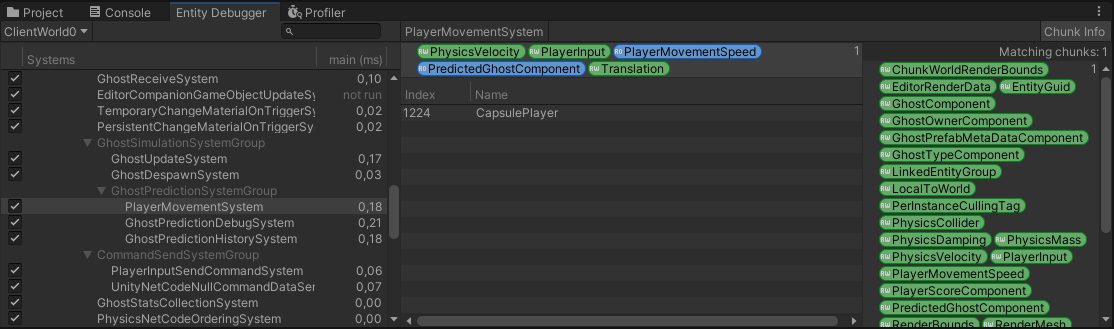
\includegraphics[width=0.95\columnwidth]{gfx/imgs/chapter2/EntityDebugger.png}
    \caption{Entity Debugger in Play Mode che mostra i sistemi in esecuzione in ClientWorld0.}
    \label{fig:entity-debugger}
\end{figure}

\subsection{Ordine di aggiornamento dei sistemi}
Generalmente i sistemi vengono aggiornati nell'ordine in cui sono inseriti nel gruppo padre. Per modificare manualmente l'ordine, possiamo utilizzare gli attributi \verb|[UpdateBefore]| e \verb|[UpdateAfter]| che indicano rispettivamente prima e dopo quale gruppo il sistema dev'essere aggiornato. Inoltre, possiamo specificare il gruppo padre con l'attributo \verb|[UpdateInGroup]|.
ECS di default crea una gerarchia di gruppi e sistemi che si dirama da tre nodi principali per tre particolari fasi del player loop (il ciclo di esecuzione della Play Mode):
\begin{itemize}
    \item \verb|InitializationSystemGroup|. Aggiornato alla fine della fase Initialization del player loop.
    \item \verb|SimulationSystemGroup|. Aggiornato alla fine della fase Update del player loop.
    \item \verb|PresentationSystemGroup|. Aggiornato alla fine della fase PreLateUpdatee del player loop.
\end{itemize}

Questa gerarchia non è statica, sia perché possiamo modificarla aggiungendo gruppi e sistemi, sia perché con certi package Unity aggiunge ulteriori gruppi. Ad esempio, utilizzando NetCode, vengono aggiunti i gruppi \verb|ClientSimulationSystemGroup| e \verb|ServerSimulationSystemGroup| che si occupano di aggiornare la simulazione rispettivamente solo sui client e solo sul server~\cite{article:player-loop-groups, doc:unity-entities-manual}.

\subsubsection{Entity Command Buffer}
Gli \verb|EntityCommandBuffer| sono strutture che permettono di accodare dei comandi eseguiti sul main thread o un job, così che possano essere eseguiti più avanti sul main thread e tutti insieme nello stesso frame.
Lo scopo di questa classe è risolvere due principali problemi: 
\begin{enumerate}
    \item All'interno di un job non è possibile accedere all'\verb|EntityManager| (quindi nemmeno all'interno di \verb|Entities.ForEach|).
    \item Quando viene eseguita un'operazione che causa un \emph{cambiamento strutturale} si genera un \emph{punto di sincronizzazione}.
\end{enumerate}

Il modo più efficiente di usare gli \verb|EntityCommandBuffer| è sfruttare uno dei tanti sistemi che li gestiscono, ad esempio \verb|EntityCommandBufferSystem|. Questi forniscono delle istanze di oggetti \verb|EntityCommandBuffer|, utilizzabili anche all'interno di altri sistemi, i cui comandi verranno eseguiti in sequenza nell'ordine in cui vengono inseriti. Nel caso ci servisse più di un buffer, i sistemi EntityCommandBufferSystem li gestiscono eseguendoli nell'ordine in cui sono stati creati.
Questo ci permette di creare un singolo punto di sincronizzazione quando \verb|EntityCommandBufferSystem| viene aggiornato, piuttosto che uno per ogni \verb|EntityCommandBuffer|, e garantisce determinismo.\\
Nel caso il job esegua in parallelo (ad esempio tramite \verb|ScheduleParallel()|), dobbiamo convertire l'\verb|EntityCommandBuffer| in uno concorrente, utilizzando il metodo \verb|AsParallelWriter()|~\cite{doc:unity-entities-api}.

\SaveVerb{EntityCommandBufferTerm}|EntityCommandBuffer|
\SaveVerb{OnUpdate()Term}|OnUpdate()|

\begin{lstlisting}[caption={Esempi di utilizzo di \UseVerb{EntityCommandBufferTerm}.}, label={lst:entitycommandbuffer-example}, language={[Sharp]C}]
var commandBuffer;

// esempio di creazione manuale di un command buffer
commandBuffer = new EntityCommandBuffer(Allocator.Temp);

// esempi di ottenimento di un command buffer da un sistema che li gestisce
commandBuffer = World.GetOrCreateSystem<EntityCommandBufferSystem>();
commandBuffer = World.GetOrCreateSystem<EndSimulationEntityCommandBufferSystem>();
commandBuffer = 
    World.GetOrCreateSystem<BeginInitializationEntityCommandBufferSystem>();

// creazione di un'entita' vuota e aggiunta di componenti
Entity ent = commandBuffer.CreateEntity();
commandBuffer.SetComponent(ent, new PlayerMovementSpeed() { speed = 10.0 });

// le operazioni seguenti non sono necessarie nel caso abbiamo ottenuto il buffer
// tramite uno dei sistemi descritti in precedenza.

// esegue in ordine tutte le operazioni accumulate nel buffer e ne libera la memoria
commandBuffer.PlayBack(EntityManager);
commandBuffer.Dispose();
\end{lstlisting}

\subsubsection{Punti di sincronizzazione}
Un punto di sincronizzazione è un momento nell'esecuzione del programma in cui aspettiamo il termine di tutti i job che sono stati schedulati prima. Essi impediscono di utilizzare tutti i worker thread disponibili nel job system per un certo periodo di tempo, perciò è meglio evitarli.
I punti di sincronizzazione sono causati principalmente dai cambiamenti strutturali, ovvero quelle operazioni che modificano l'archetipo di un'entità o cambiano l'ordine delle entità in un chunk. Esempi di cambiamenti strutturali sono la creazione e l'eliminazione di entità, l'aggiunta e la rimozione di componenti da un'entità e il cambiamento del valore dei componenti condivisi~\cite{doc:unity-entities-manual}. Per evitare i punti di sincronizzazione è possibile eseguire le operazioni che causano cambiamenti strutturali tutte insieme, tramite un \verb|EntityCommandBuffer|.

%\subsubsection{Job generici} % utile per prototipo? RICONTROLLARE
% Non serve perché li uso solo nei prototipi per gli stress test ma solo per creare le entities, non per mostrare il carico del lavoro. Per questo basta la parte sui system che fa ECS in background (.Run(), .Schedule() e .ScheduleParallel() sulla lambda)


%%%%%%%%%%%%%%%%%%%%%%%%%%%%%%%%%%%%%%%%%%%%%%%%%%%%%%%%%%%%%%%%%%%%%%%%%%%%%
\section{Conversion Workflow}
Unity ECS fornisce un meccanismo di conversione che permette di trasformare i GameObject (ed i MonoBehaviour associati), presenti in una scena, in entità. La differenza principale quando usiamo DOTS invece dell'architettura classica di Unity, è che invece di implementare dati e logica nei MonoBehaviour, definiamo i componenti per memorizzare dati a runtime e scriviamo i sistemi per realizzare la logica.

Per convertire un GameObject esistono due soluzioni: possiamo aggiungervi il componente \verb|ConvertToEntity| (MonoBehaviour), oppure inserirlo in una subscene. In entrambi i casi i sistemi di conversione forniti da DOTS processano il GameObject o il Prefab e tutti gli oggetti figli e li converte.
Tuttavia, la seconda soluzione è da preferire, in quanto con la subscene ECS serializza e salva su disco i dati delle entità che genera durante la conversione. Tali dati possono essere caricati o trasmessi in stream molto velocemente a tempo di esecuzione, e possiamo anche abilitare e disabilitare le singole subscene fra authoring data e runtime data, per ``mantenere attivi'' solo gli elementi su cui si sta lavorando al momento (ciò è indispensabile nel caso di progetti di grandi dimensioni, con molti GameObject). Al contrario, con il componente \verb|ConvertToEntity|, un GameObject viene convertito solamente a tempo di esecuzione.

Solitamente utilizziamo le subscene per convertire tutto ciò che DOTS può convertire, mentre lasciamo fuori gli elementi che non hanno ancora un corrispondente in ECS (ad esempio le luci o la camera). Così facendo possiamo ottenere i benefici della scalabilità offerti da DOTS solo sugli elementi rilevanti dell'applicazione.

\subsubsection{Generazione di Authoring component}
Per componenti semplici possiamo utilizzare l'attributo \verb|[GenerateAuthoringComponent]| per fare in modo che Unity generi automaticamente il componente ECS relativo. Quando ciò avviene, Unity crea una classe \verb|MonoBehaviour| che contiene i campi pubblici del componente ed implementa un metodo che converte questi campi in runtime data del componente, di conseguenza è possibile aggiungere lo script direttamente al GameObject nell'editor e vederlo nell'Inspector.

\SaveVerb{[GenerateAuthoringComponent]Term}|[GenerateAuthoringComponent]|

\begin{figure}[!ht]
    \centering
    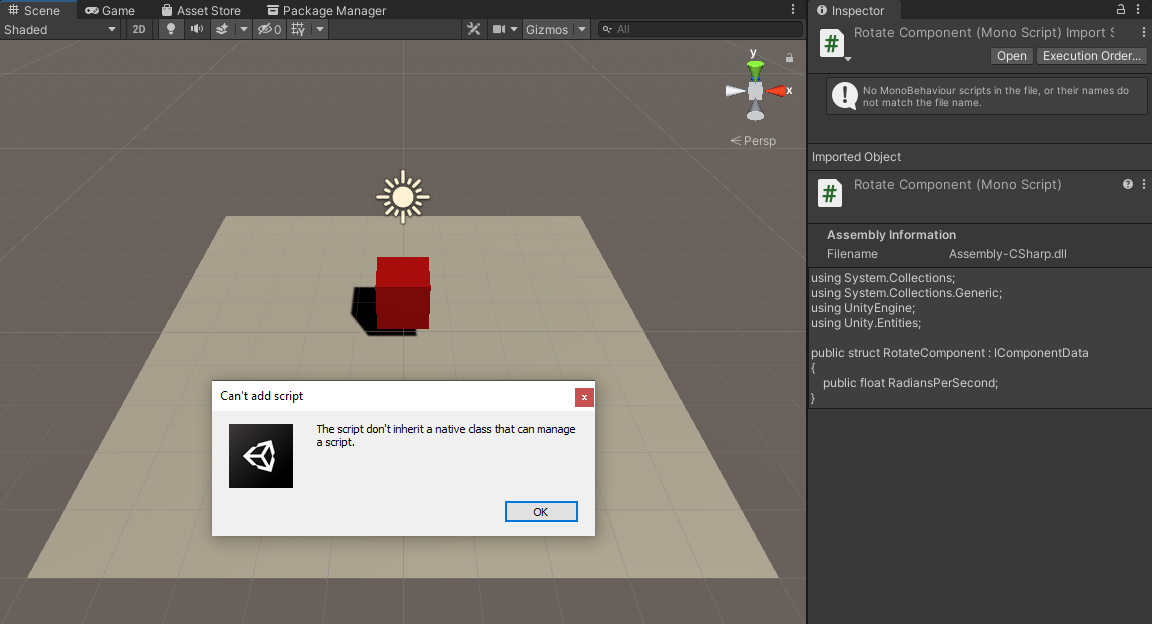
\includegraphics[width=0.95\columnwidth]{gfx/imgs/chapter2/NonAuthoringComponentExample.png}
    \caption{Componente senza tag \UseVerb{[GenerateAuthoringComponent]Term}.}
    \label{fig:non-authoring-example}
\end{figure}

\begin{figure}[!ht]
    \centering
    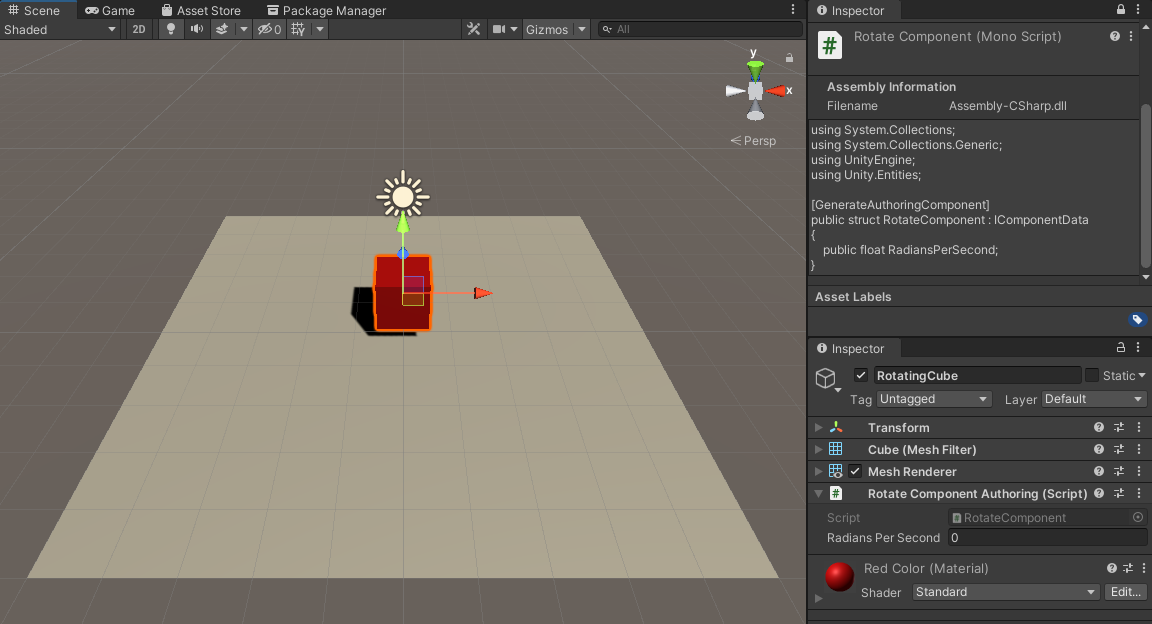
\includegraphics[width=0.95\columnwidth]{gfx/imgs/chapter2/AuthoringComponentExample.png}
    \caption{Componente con tag \UseVerb{[GenerateAuthoringComponent]Term}.}
    \label{fig:authoring-example}
\end{figure}

\subsubsection{Sistemi di conversione}
I sistemi di conversione ereditano dalla classe \verb|GameObjectConversionSystem| e permettono di convertire GameObject ed asset in entità. Di default aggiornano nel gruppo \verb|GameObjectConversionGroup| e una delle differenze più consistenti rispetto ai sistemi normali di ECS è che quelli di conversione non si trovano in un World singolo ma stanno a cavallo di due: leggono dal Conversion World (quello in cui si trovano gli authoring data) e scrivono nel Destination World (in cui si trovano le entità).

Durante la conversione, per ogni GameObject processato viene creata l'entità corrispondente.
Inoltre, i sistemi di conversione eseguono sul main thread senza burst, infatti il costrutto \verb|Entities.ForEach| non richiede la chiamata a metodi \verb|Run()| o \verb|Schedule()| quando viene utilizzato all'interno di questi~\cite{doc:unity-entities-api}.

\subsubsection{Interfaccia IConvertGameObjectToEntity}
Un metodo più semplice rispetto alla creazione di un sistema di conversione consiste nell'implementare l'interfaccia \verb|IConvertGameObjectToEntity| nella classe del \verb|MonoBehaviour| contenente il componente. Questa interfaccia fornisce un metodo con il quale possiamo realizzare una conversione personalizzata. Praticamente permette di personalizzare ciò che l'attributo \verb|[GenerateAuthoringComponent]| realizza in modo trasparente.

Durante l'aggiornamento del gruppo \verb|GameObjectConversionGroup|, viene chiamato il metodo \verb|Convert()| di tutti i componenti che implementano questa interfaccia ~\cite{doc:unity-entities-manual}.

\SaveVerb{IConvertGameObjectToEntityTerm}|IConvertGameObjectToEntity|

\begin{lstlisting}[caption={Esempio di conversione personalizzata tramite l'utilizzo dell'interfaccia \UseVerb{IConvertGameObjectToEntityTerm}~\cite{youtube:conversione-dati-scene-dots}.}, label={lst:convert-example}, language={[Sharp]C}]
public struct RotateComponent : IComponentData
{
	public float RadiansPerSecond;
}

public class RotateComponentAuthoring : MonoBehaviour, IConvertGameObjectToEntity
{
	public float DegreesPerSecond

	public void Convert(Entity entity, EntityManager dstManager, GameObjectConversionSystem conversionSystem)
	{
		dstManager.AddComponentData(entity, 
		new Rotate { RadiansPerSecond = math.radians(DegreesPerSecond) });
	}
}
\end{lstlisting}

%subsubsection{Prefabs}

%\subsubsection{Conversione in LiveLink} % forse non serve, nel prototipo non è stato utilizzato (volendo c'è scritto qualcosa di veloce nella descrizione del package Entities)
% IJobEntityBatch (API) c'è scritta molta roba utile       % 2.Unity ECS
\cleardoublepage

\chapter{Unity DOTS: NetCode}
\label{cap:netcode}
Assieme allo sviluppo dell'architettura data-oriented introdotta con DOTS, si è reso necessario implementare dei meccanismi che permettessero di utilizzare il modello di ECS anche nella comunicazione in rete.
Il package NetCode permette di realizzare un design di rete a server dedicato con predizione lato client, in cui lo scambio di messaggi avviene tramite entità, componenti e sistemi. Il funzionamento di NetCode si basa su API di più basso livello fornite dal package Transport, il quale sostituisce la vecchia libreria di Unity per il networking.
In questo capitolo forniremo un'infarinatura sullo sviluppo di videogiochi multiplayer assieme ad un background sulle possibili problematiche introdotte con il networking. Infine, mostreremo le soluzioni proposte e le scelte attuate da Unity per la realizzazione dei package DOTS relativi al multiplayer.

\section{Background sullo sviluppo di giochi multiplayer}
Quando parliamo di sviluppo di giochi multiplayer è necessario avere ben chiaro in mente come funziona la comunicazione in Internet e scegliere la soluzione migliore per il tipo di gioco che si vuole realizzare. A tal proposito è importante conoscere le principali topologie di rete, i protocolli utilizzati ed i problemi che possono occorrere.

\subsubsection{Topologie di rete}
I videogiochi multiplayer possono essere strutturati in diversi modi, ognuno dei quali con i propri vantaggi e svantaggi, ed ognuno adatto a tipi di giochi differenti.

\paragraph{Locale}
È la tipologia più semplice. Il gioco esegue su una singola macchina, di conseguenza l'unico codice da implementare è quello del client. La differenza rispetto ad un videogioco singleplayer è che il gioco in locale riceve e deve processare diversi input, in quanto ci sono più giocatori. Tra i vantaggi di questa topologia di rete spiccano la latenza prossima a zero, la sicurezza e la complessità minima del modello. Tuttavia, è una soluzione poco scalabile in quanto di norma non consente la partecipazione di più di 4 giocatori, i quali devono trovarsi nella stessa stanza. Dunque, solitamente viene utilizza per giochi semplici, quali platform e puzzle games in schermo condiviso o split screen~\cite{youtube:realtime-multiplayer}.

\paragraph{LAN}
Anche questo modello è offline ma, al contrario del precedente, permette di connettere diversi dispositivi. Ai vantaggi dei giochi in locale aggiunge la scalabilità: infatti, tramite questa soluzione è possibile raggiungere anche centinaia di giocatori. In ogni caso, persiste il problema che i partecipanti devono essere vicini e raggiungibili. Ultimamente viene utilizzata soprattutto per i giochi che utilizzano la realtà virtuale, in quanto è necessaria una latenza minima~\cite{youtube:realtime-multiplayer}.

\paragraph{Peer-to-peer}
È una topologia di rete che sfrutta la connessione ad Internet, in cui tutti i giocatori che partecipano alla sessione di gioco sono collegati fra loro. Poiché ogni peer ha \emph{O(n - 1)} connessioni, dove \emph{n} è il numero di peer, questa soluzione è poco scalabile, in quanto maggiore è il numero di peer collegati, maggiore sarà la banda di rete richiesta. Inoltre, con questa soluzione vi è \emph{input sharing}, ovvero ogni peer deve ricevere e processare gli input di tutti gli altri. Di conseguenza, è necessario mantenerli sincronizzati per evitare che la latenza di uno provochi il disallineamento delle simulazioni di gioco. Ciò rende la logica alla base di questo modello sorprendentemente complessa da implementare. Solitamente questa soluzione viene utilizzata in giochi in cui le partite vengono disputate fra un numero ristretto di partecipanti~\cite{book:multiplayergameprogramming}.

\paragraph{Client$/$Server}
il design di questa rete prevede una separazione del codice di gioco fra client e server. Ogni client comunica solo con il server, mentre il server deve comunicare con tutti i client collegati. Quindi, il server deve mantenere \emph{O(n)} connessioni, dove \emph{n} è il numero di client, mentre ogni client mantiene una sola connessione, verso il server. Fra i vantaggi di questa soluzione vi è il fatto che i client non devono processare gli input di tutti gli altri client, ma ricevono solo gli aggiornamenti del server. Inoltre, la banda richiesta non aumenta con il numero di client, se non di valori irrilevanti dovuti alle dimensioni dello stato di gioco ricevuto (più client ci sono, più oggetti da replicare dovranno essere trasmessi)~\cite{book:multiplayergameprogramming}.

\paragraph{Sottocategorie}
Oltre a queste macro categorie esistono anche delle sottocategorie, in particolare per il modello Client/Server.
Un'architettura di tipo \emph{Listen server} è un modello a Client/Server in cui un client diventa server e ospita la partita per tutti gli altri client. I problemi principali consistono nel fatto che l'host è privilegiato in quanto non ha latenza. Di conseguenza, è necessario implementare un sistema di migrazione dell'host in caso questo si disconnetta, creando situazioni spiacevoli in cui tutti devono aspettare.

\begin{figure}[!ht]
    \begin{subfigure}{.49\textwidth}
      \centering
      % include first image
      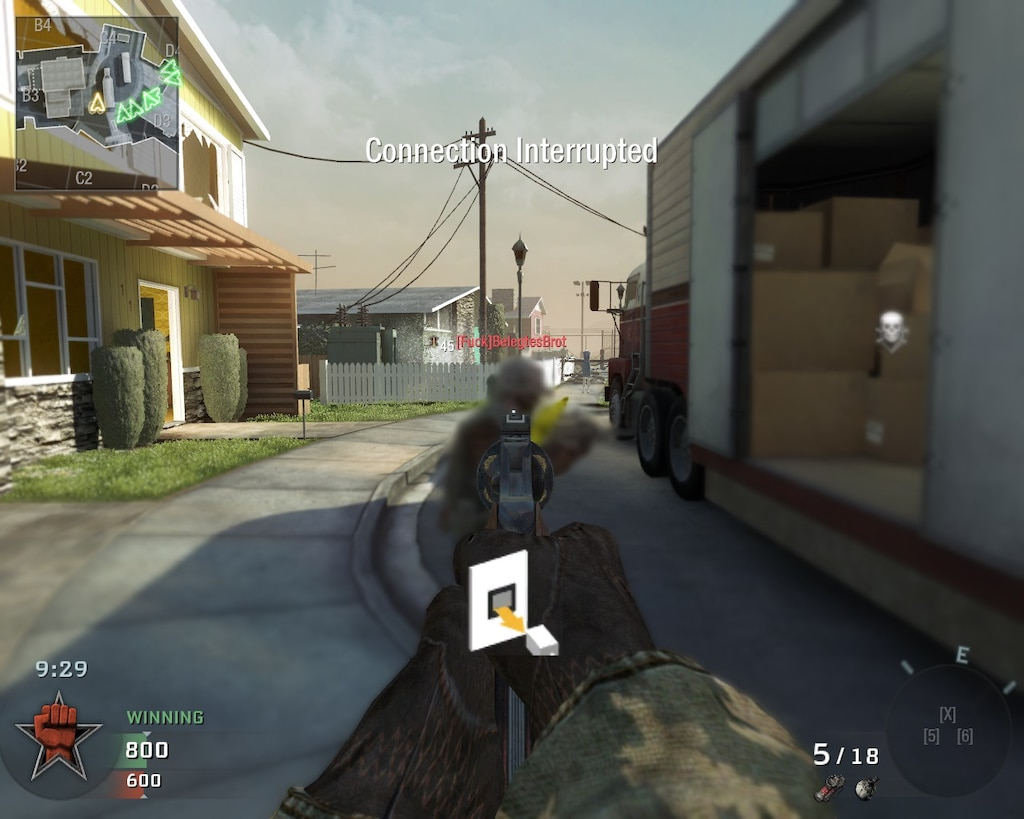
\includegraphics[width=.95\linewidth]{gfx/imgs/chapter3/CoDBOConnectionInterrupted.png}
      \caption{Connessione Interrotta.}
      \label{fig:connection-interrupted}
    \end{subfigure}
    \begin{subfigure}{.49\textwidth}
      \centering
      % include second image
      
\includegraphics[width=.95\linewidth]{gfx/imgs/chapter3/CoDBO2MigratingHosts.png}
      \caption{Migrazione Host.}
      \label{fig:host-migration}
    \end{subfigure}
    \caption{Esempi di problemi di connessione nei giochi multiplayer con riferimento a Call of Duty.}
    \label{fig:multiplayer-problems}
\end{figure}

Nel modello a \emph{Server dedicato} vengono utilizzati server ospitati, solitamente forniti da servizi di hosting, per cui il controllo è totalmente nelle mani dello sviluppatore, invece che dei giocatori. Questo permette di fare delle scelte specifiche in base al target del gioco, ad esempio possiamo scegliere server più o meno potenti e distribuirli maggiormente in giro per il mondo man mano che il gioco cresce in popolarità. Tipicamente questa soluzione prevede che il server sia headless, ovvero non sfrutta alcuni moduli quali il sistema di rendering grafico, in quanto non ha bisogno di renderizzare nulla ma solo mantenere in esecuzione la simulazione principale.

Esiste inoltre il modello a \emph{Server autoritativo}, nel quale vengono eseguiti due tipi di simulazione, ma l'unica da considerare sempre corretta è quella del server. Di conseguenza, se per qualche motivo il client dovrebbe trovarsi in uno stato incerto, aggiornerà il proprio stato in base a ciò che riceve dal server. Ciò limita molto la possibilità di utilizzo di hack o cheat per ottenere vantaggi rispetto agli altri giocatori~\cite{book:multiplayergameprogramming, youtube:realtime-multiplayer}.

Gli ultimi due modelli solitamente vengono utilizzati insieme e rappresentano una soluzione estremamente scalabile, ideale per giochi le cui partite vengono disputate da un numero di partecipanti molto elevato, ad esempio i battle royale, che possono arrivare anche a più di 100 giocatori connessi contemporaneamente. Fra gli svantaggi principali vi sono: i costi, in quanto per progetti di grandi dimensioni solitamente è necessario affidarsi a servizi di hosting o data center; la latenza dovuta al fatto che, essendo i client connessi fra di loro indirettamente tramite il server, i messaggi devono prima passare da quest'ultimo, per essere ricevuti dagli altri. Per questo motivo solitamente si cerca di implementare un sistema di matchmaking che privilegi le connessioni fra client ``limitrofi''.
Il modello a server dedicato autoritativo è di particolare interesse ai fini della tesi, in quanto rappresentano l'architettura scelta da Unity per lo sviluppo della nuova libreria di networking introdotta con DOTS.

\begin{figure}[!ht]
    \begin{subfigure}{.49\textwidth}
      \centering
      % include first image
      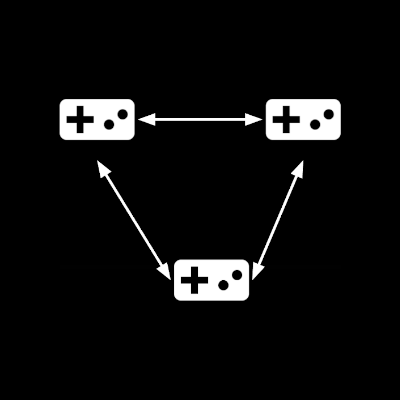
\includegraphics[width=.95\linewidth]{gfx/imgs/chapter3/PeerToPeerSchema.png}
      \caption{Peer-to-peer.}
      \label{fig:peer-to-peer}
    \end{subfigure}
    \begin{subfigure}{.49\textwidth}
      \centering
      % include second image
      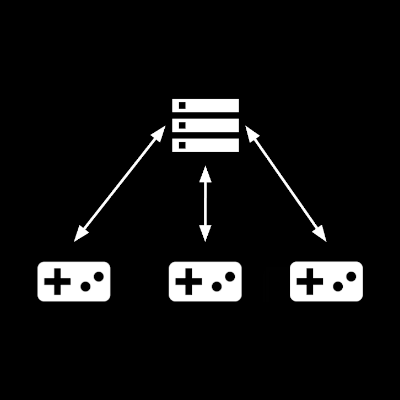
\includegraphics[width=.95\linewidth]{gfx/imgs/chapter3/DedicatedServerSchema.png}
      \caption{Server dedicato.}
      \label{fig:dedicated-server}
    \end{subfigure}
    \caption{Schemi delle connessioni dei due modelli più utilizzati.}
    \label{fig:authoritative-server}
\end{figure}

\subsubsection{Transport layer e protocolli UDP e TCP}
Nello sviluppo di un videogioco multiplayer, il livello più basso dello stack di rete con cui è possibile sporcarsi le mani è il transport layer (tutto il resto viene svolto dall'architettura sottostante e dall'hardware). A questo livello si trovano le socket, che permettono di stabilire un canale di comunicazione tra due end-point e utilizzano due protocolli principali:

\paragraph{TCP}
È orientato alla connessione e garantisce affidabilità, ovvero che i pacchetti arrivino sempre, in ordine e senza essere duplicati. Per questo motivo i pacchetti TCP hanno un header pesante (le dimensioni variano da 20 a 60 byte) che contiene diverse informazioni, molte delle quali sono inutili ai fini del gioco che si vuole implementare. Inoltre, per come è realizzato TCP, nel caso un pacchetto venga perso, viene richiesta una ritrasmissione e questo genera latenza extra assolutamente non tollerabile in un gioco in tempo reale. Come se ciò non bastasse, con TCP la perdita di pacchetti c'è sempre, poiché dispone di un meccanismo di controllo di congestione, il cui algoritmo prevede che la velocità di trasmissione aumenti sempre finché non viene perso un pacchetto, per poi diminuire e ricominciare ad aumentare gradualmente~\cite{standard:rfc5681}.

\paragraph{UDP}
È leggero e molto più veloce, in quanto non dà alcun tipo di garanzia e, di conseguenza, ha un header di dimensioni ridotte (8 byte). Infatti, con questo protocollo i pacchetti non vengono tracciati e, nel caso un pacchetto venga perso, nessuno se ne accorge e la comunicazione continua. Nel caso fossero necessarie particolari specifiche di affidabilità, bisognerebbe implementarle manualmente.

\paragraph{Cosa scegliere}
Poiché in un videogioco l'aspetto più importante è garantire un'esperienza di gioco ottimale per tutti, la scelta del protocollo assume particolare rilevanza. Solitamente utilizziamo TCP solo nei giochi a turni, perché la latenza non permette di avere una risposta soddisfacente da parte del server. Dunque, la scelta più gettonata è UDP, a cui di norma aggiungiamo l'implementazione di qualche tecnica per evitare che i pacchetti vengano riordinati, arrivino duplicati, oppure vengano persi.

\subsubsection{Problematiche di rete nei videogiochi multiplayer}
Indipendentemente dal tipo di gioco, per quanto la tecnologia si sia evoluta negli ultimi decenni, possono verificarsi comunque dei problemi dovuti ai limiti fisici dell'hardware (schede di rete obsolete, router eterogenei, cavi datati) e alla velocità con cui possono essere trasmessi i dati (connessioni limitate, banda di rete condivisa).
Per questo motivo è importante progettare l'applicazione tenendo conto delle diverse problematiche che possono avere un impatto negativo sull'esperienza di gioco.
\paragraph{Latenza, Jitter e Perdita di pacchetti}
Quando un gioco viene testato in rete locale alcuni dei fattori che influenzano negativamente il gioco non sono presenti. Quando però il gioco viene rilasciato, possono verificarsi i seguenti:
\begin{itemize}
    \item Latenza. Si riferisce al tempo che impiega un pacchetto ad essere trasferito dal nodo sorgente a quello di destinazione. Questo ritardo impone un limite inferiore alla velocità con cui le informazioni e lo stato di gioco possono essere scambiate fra due end-point, condizionando di conseguenza la possibilità dei giocatori di reagire a cambiamenti situazionali.
    \item Jitter. consiste nella variazione di latenza fra un pacchetto ed il seguente. Questo può essere un problema ad esempio per i giocatori (o anche per il game engine stesso) che non riescono a compensare la latenza a medio o lungo termine della rete.
    \item Perdita di pacchetti. si verifica quando un pacchetto non raggiunge mai la destinazione. Se degli aggiornamenti dello stato del gioco vengono persi, il game engine deve sistemare il danno come meglio può per fare in modo che la simulazione non risulti compromessa e sia comunque fluida e giocabile.
\end{itemize}

Le cause di queste problematiche possono essere differenti. Sebbene molte siano dovute a limiti hardware non risolvibili, altre possono essere aggirate o attenuate tramite l'utilizzo di particolari tecniche o meccanismi implementativi durante lo sviluppo dell'applicazione.
Inoltre, a seconda del tipo di gioco che stiamo sviluppando, le problematiche definite precedentemente possono incidere in modi differenti, più o meno tollerabili. Ad esempio, una latenza considerevole, di addirittura 500ms, è accettabile in alcuni RTS\footnote{Nei giochi \emph{Real-Time Strategy} il giocatore solitamente controlla delle unità assegnandovi delle azioni da svolgere.}, mentre generi come gli FPS, i MOBA\footnote{Nei \emph{First-Person Shooter} e \emph{Multiplayer Online Battle Arena}, il giocatore controlla un singolo personaggio, dunque è necessaria una risposta molto rapida ai comandi.} ed i picchiaduro necessitano di valori attorno ai 30ms (in generale non oltre i 50ms), per non rovinare l'esperienza di gioco~\cite{book:networkingandonlinegames, book:multiplayergameprogramming}.

\paragraph{Tecniche per migliorare la latenza}
La latenza è un problema che esiste sempre e non è possibile eliminarlo a priori. Tuttavia, possiamo utilizzare delle tecniche per aggirarla e migliorare, almeno in parte, l'esperienza di gioco. Ad esempio, poiché il flusso di gioco solitamente non è costante (gli aggiornamenti inviati dal server non arrivano con la stessa frequenza), questo potrebbe causare una percezione fastidiosa da parte del giocatore, che vedrebbe il gioco eseguire a scatti. A tal proposito esiste una tecnica chiamata \emph{interpolazione lato client}, che permette di smussare il flusso di gioco. Ciò allevia la sensazione di latenza che questa condizione genera, rendendo il gioco più fluido. Infatti, tramite questo metodo, quando il client riceve uno stato dal server non lo presenta subito, ma calcola l'interpolazione tra l'ultimo stato ricevuto ed il precedente, utilizzando un filtro di percezione locale.

Tuttavia, l'interpolazione migliora l'esperienza di gioco, ma non avvicina ciò che il giocatore vede a ciò che effettivamente sta succedendo lato server. Anche se il periodo di interpolazione fosse breve, lo stato di gioco sarebbe comunque più vecchio di 1/2 RTT\footnote{Round Trip Time (RTT): somma del tempo che impiega un pacchetto a transitare in rete dal nodo mittente al ricevente ed il tempo che impiega il pacchetto di risposta (ad esempio un ACK che conferma la ricezione) a tornare sul nodo iniziale. Si misura in millisecondi.} rispetto a quello del server.

Per riuscire a mostrare uno stato di gioco che sia più corretto, è necessario utilizzare la \emph{predizione lato client}, che viene attuata tramite l'estrapolazione. Per farlo è necessario che il client esegua la stessa simulazione del server e, quando riceve un aggiornamento da quest'ultimo, sa che è datata di 1/2 RTT. Dunque, per rendere lo stato più corretto, il client esegue la simulazione per un ulteriore 1/2 RTT. Così facendo, quando il client presenta la simulazione al giocatore, è un'approssimazione molto più veritiera di ciò che sta effettivamente succedendo lato server. Per mantenere l'approssimazione, il client continua ad eseguire la simulazione ogni frame e mostrare il risultato al giocatore. Poi, quando riceve un nuovo stato dal server, internamente lo simula per 1/2 RTT che, idealmente, a questo punto corrisponde allo stato esatto che il client ha già calcolato in base al precedente~\cite{book:multiplayergameprogramming}.

\subsubsection{Soluzione proposta da Unity}
Con l'introduzione di DOTS, la vecchia libreria per il networking UNet è diventata obsoleta e serviva qualcosa di più adeguato all'architettura basata sul modello orientato ai dati di ECS. A tal proposito Unity ha inserito nello stack due package, con l'obbiettivo di realizzare una comunicazione performante e scalabile (sul modello di DOTS), che fosse compatibile fra piattaforme eterogenee e che fosse, inoltre, modulare e trasparente:
\begin{itemize}
    \item \textbf{Transport}. Questo package è implementato sfruttando il protocollo UDP, in quanto estremamente semplice e veloce, aggiungendovi però alcune funzionalità. In particolare, sono state inserite utilità per: pacchettizzare i dati da inviare ad ogni frame di gioco, tramite un buffer; gestire le connessioni, permettendo di avere qualche garanzia in più ad esempio sul fatto che il server esista effettivamente, oppure che si ottenga una notifica in caso il server vada offline o non sia più raggiungibile; integrare il sistema di networking con il job system di unity, permettendo di eseguire le simulazioni di rete su thread multipli oppure, anche nel caso in cui si stia utilizzando un server a thread singolo, ottenere tutti i benefici della compilazione con burst~\cite{youtube:unity-transport}.
    \item \textbf{NetCode}. Questo package è stato pensato per sviluppare principalmente giochi in tempo reale, i quali impongono requisiti di latenza contenuta. A tal proposito è stato realizzato sul modello a server dedicato con server autoritativo, utilizzando le API fornite dal Transport package. Per attenuare il problema della latenza è stata introdotta la predizione lato client. In questo modo l'esperienza di gioco risulta fluida e piacevole~\cite{youtube:unity-netcode}.
\end{itemize}

%%%%%%%%%%%%%%%%%%%%%%%%%%%%%%%%%%%%%%%%%%%%%%%%%%%%%%%%%%%%%%%%%%%%%%%%%%%%%
% roba più pratica con costrutti e come funzionano spiegati nel dettaglio
\section{Transport package}
Il package \emph{Transport} (com.unity.transport) è stato realizzato per sostituire le API di basso livello della vecchia libreria UNet per il networking, ormai diventata obsoleta. Contiene costrutti e metodi utili alla serializzazione degli stream di dati da inviare in rete, permettendo di stabilire connessioni e spedire messaggi ad host remoti.

\subsubsection{Scambio di messaggi}
La comunicazione in questo package si basa su un modello ad eventi, i quali danno informazioni sullo stato della connessione (ad esempio indicano se ci sono messaggi da leggere). I dati vengono trasmessi in rete a blocchi e, quando si vuole costruire un sistema di comunicazione, è necessario tenere conto dell'allineamento in memoria e dell'ordine dei byte (Endianness), il quale può variare fra dispositivi eterogenei~\cite{doc:microsoft-memory-alignment, youtube:unity-transport}. Per questo motivo, il Transport package fornisce dei costrutti che permettono di bufferizzare i dati senza dover tenere in considerazione tutte queste convenzioni, in quanto l'implementazione sottostante fa già tutto per noi:
\begin{itemize}
    \item \verb|DataStreamWriter|. Permette di allocare un buffer di memoria e supporta scritture di tipo deferred. È possibile utilizzarlo per serializzare i dati da inviare ed essendo una struttura non è gestito da un garbage collector.
    \item \verb|DataStreamReader|. È la controparte del precedente e permette di deserializzare i dati ricevuti. È ciò che si ottiene quando si riceve un evento dalla rete e permette di leggere i dati ricevuti, accumulati in un buffer. Al contrario del precedente è una struttura \emph{immutabile}. Di conseguenza, tutto lo stato contenuto dev'essere memorizzato in un context esterno, altrimenti non sarebbe possibile aggiornare la posizione di lettura e bisognerebbe specificare gli offset dei byte manualmente (operazione estremamente prona ad errori).
\end{itemize}

\subsubsection{Gestione delle connessioni}
Per realizzare lo scambio di messaggi tra due endpoint si utilizza la struttura \verb|NetworkDriver|, che implementa le connessioni virtuali a livello del transport layer sia per i client che per il server(host).
Una connessione virtuale è rappresentata da una struttura \verb|NetworkConnection|, che mantiene tutte le informazioni necessarie al driver per comunicare con l'altro endpoint ed è ottenibile connettendosi ad un server oppure accettando una connessione.

\paragraph{NetworkDriver}
\verb|NetworkDriver| è il costrutto principale del package e sfrutta l'interfaccia di rete \verb|INetworkInterface| che rappresenta la socket di basso livello, per inviare e ricevere dati. Contiene metodi per creare il driver, eseguire il binding (con UNet questo veniva fatto in automatico), connettersi a un server dal client, accettare le connessioni dei client dal server, inviare e ricevere dati da una connessione, eseguire l'operazione di pop (ovvero leggere e rimuovere) dalla coda degli eventi di rete~\cite{doc:unity-transport-api}.

Infatti, poiché lo scambio di messaggi tra i driver di due endpoint viene notificato tramite eventi, la struttura \verb|NetworkDriver| dispone di 4 tipi di eventi differenti, contenuti nell'enumerativo \verb|NetworkEvent.Type|:
\begin{itemize}
    \item \verb|Empty| (default). Indica che non ci sono altri messaggi da leggere nella coda degli eventi, per il frame corrente.
    \item \verb|Data|. Indica che sono stati ricevuti dei dati da un endpoint connesso ed è possibile leggerli mediante \verb|DataStreamReader|.
    \item \verb|Connect|. Indica che è stata stabilita una nuova connessione (disponibile solo se il driver non si trova in stato listening).
    \item \verb|Disconnect|. Indica che è stato ricevuto un pacchetto di disconnessione, si è verificato un timeout della socket, oppure è stato raggiunto il limite massimo di tentativi di connessione a \verb|NetworkConnection|.
\end{itemize}

Questi eventi sono i medesimi sia per client che per server, l'unica differenza è come vengono consumati~\cite{doc:unity-transport-manual}.

Inoltre, il driver dispone di un metodo \verb|BeginSend()| che restituisce una struttura \verb|DataStreamWriter|, utilizzabile per inviare dati all'altro endpoint della connessione specificata.

Solitamente la sequenza di esecuzione del codice è:
\begin{enumerate}
    \item Il client invia un evento \verb|Connect| al server.
    \item Il server risponde con un evento \verb|ConnectionAccept|.
    \item Sia server che client possono iniziare subito a trasmettere dati.
    \item Il server invia un evento \verb|Disconnect| e la comunicazione termina.
\end{enumerate}

Poiché il transport package è realizzato utilizzando UDP, è possibile che un pacchetto venga perso. Nel caso venisse perso il messaggio \emph{Connect}, è presente un timeout dopo il quale, se non viene ricevuta risposta dal server, ne viene inviato un altro. Così facendo ci si assicura che la connessione venga effettivamente stabilita. Nel caso a essere perso fosse, invece, il messaggio \emph{ConnectionAccept}, avviene una connessione implicita, con cui il client capisce che la connessione è stata accettata, al primo pacchetto contenente dei dati ricevuto dal server.

Il motivo per cui non è possibile inviare dati prima della conferma della connessione, è dovuto al fatto che il package Transport supporta connessioni multiple dei client al medesimo server. Di conseguenza, è necessario un meccanismo per identificare le connessioni dei vari client e che le mantenga ``up-to-date'': ogni client assieme al messaggio di richiesta della connessione invia un token identificiativo, al quale il server risponde col proprio token. Senza la conoscenza dei reciproci token, la comunicazione non può avvenire~\cite{youtube:unity-transport}.

\subsubsection{Integrazione con Unity Job System}
Il package Transport è stato realizzato per essere compatibile col modello di ECS e con il job system: i costrutti principali sono infatti strutture blittable, che permettono di ottenere tutti i benefici offerti dalla tecnologia DOTS, fra cui la possibilità di utilizzare il burst compiler.
A tal proposito, è possibile scaricare il lavoro del network driver, che normalmente verrebbe svolto tutto sul main thread, in job secondari, permettendo di dedicare più spazio (in un frame) alla logica di gioco. Inoltre, è anche possibile gestire le varie connessioni in parallelo, sfruttando un job di tipo \verb|IJobParallelFor| assieme alla versione concorrente del driver \verb|NetworkDriver.Concurrent|.

Poiché \verb|NetworkDriver| viene aggiornato da un job (motivo per cui il metodo che lo esegue si chiama \verb|.ScheduleUpdate()|), è necessario aspettare che termini prima di utilizzare il driver per qualsiasi altra cosa, difatti solitamente viene effettuata una chiamata al metodo \verb|.Complete()| all'inizio del ciclo di update~\cite{doc:unity-transport-manual, youtube:unity-transport}.

%L'integrazione col job system permette di eseguire tutte le simulazioni in rete su thread multipli. Inoltre, anche se si sta utilizzando un server a thread-singolo, o per un qualsiasi motivo (magari risparmiare a livello economico, utilizzando meno risorse CPU) è necessario utilizzare un singolo core, utilizzare il Job System permette di compilare il codice con burst, ottenendo un ingente miglioramento di prestazioni.

%%%%%%%%%%%%%%%%%%%%%%%%%%%%%%%%%%%%%%%%%%%%%%%%%%%%%%%%%%%%%%%%%%%%%%%%%%%%%
\section{NetCode package}
Il package \emph{NetCode} (com.unity.netcode) fornisce un modello di rete a server dedicato con predizione lato client, utilizzabile per realizzare la parte multigiocatore di un videogioco. Si basa sulle API del package Transport per le funzionalità a livello di socket, il quale è stato realizzato per essere compatibile ed ottimizzato per ECS e job system.

Al contrario di Transport, NetCode è ancora in preview, ovvero gli sviluppatori Unity stanno lavorando per migliorarlo e aggiungere ulteriori funzionalità. Pertanto, non è ancora pronto per l'utilizzo in produzione, ma è già possibile usarlo nei propri progetti~\cite{doc:unity-netcode-manual}.

\subsection{Concetti fondamentali in NetCode}

NetCode separa la logica dei client da quella del server, utilizzando world differenti per ciascuno di essi. Infatti, mentre usando semplicemente il package Entities, Unity creava un world di default in cui inizializzava ed aggiornava i vari sistemi e gruppi, con NetCode questo world viene creato comunque ma non viene utilizzato (a meno che non venga specificato diversamente). Al suo posto si utilizzano ClientWorldN dove N è il numero del client corrispondente partendo da 0, e ServerWorld, rispettivamente per la logica dei client e la logica del server.
All'interno di questi si trovano i sistemi, organizzati in gruppi specifici per l'inizializzazione, la simulazione e la presentazione. Il gruppo relativo alla presentazione è presente solo nei world client, in quanto si occupa del rendering (un frame visibile a schermo corrisponde ad una chiamata alla \verb|OnUpdate()| di questo gruppo) e di tutte quelle operazioni che servono solo ai client.

\SaveVerb{PresentationSystemGroupTerm}|PresentationSystemGroup|

\begin{figure}[!ht]
    \begin{subfigure}{.49\textwidth}
      \centering
      % include first image
      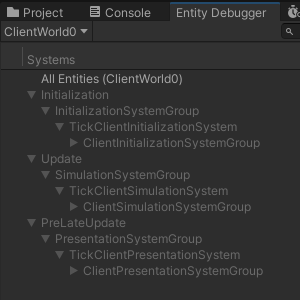
\includegraphics[width=.95\linewidth]{gfx/imgs/chapter3/SystemGroupClientNetCode.png}
      \caption{Gruppi principali nei ClientWorld.}
      \label{fig:client-world-groups}
    \end{subfigure}
    \begin{subfigure}{.49\textwidth}
      \centering
      % include second image
      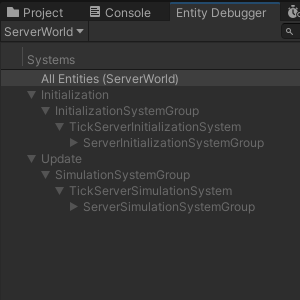
\includegraphics[width=.95\linewidth]{gfx/imgs/chapter3/SystemGroupServerNetCode.png}
      \caption{Gruppi principali nel ServerWorld.}
      \label{fig:server-world-groups}
    \end{subfigure}
    \caption{EntityDebugger: gerarchia dei gruppi principali a runtime (in ServerWorld non è presente il relativo \UseVerb{PresentationSystemGroupTerm}).}
    \label{fig:netcode-system-groups}
\end{figure}

%\paragraph{Bootstrap}
%La sequenza di bootstrap di default crea i world di client e server automaticamente all'avvio dell'applicazione, popolandoli con i sistemi definiti in base agli attributi impostati. Poiché, per vari motivi, può essere necessario ritardare la creazione dei mondi, NetCode permette di estendere la classe \verb|ClientServerBootstrap| per sovrascrivere la sequenza di bootstrap di default, fornendo metodi per la creazione del DefaultWorld e dei mondi di client e server manualmente.

\paragraph{RPC}
Le Remote Procedure Call (RPC) permettono di effettuare una chiamata ad una procedura che verrà eseguita su un dispositivo remoto. NetCode utilizza una forma limitata delle RPC per gestire degli eventi: un job che esegue sull'endpoint del mittente invia una richiesta di RPC ed un job che esegue sul lato destinatario la riceve chiamandone la funzione.

\paragraph{Ghost}
Un ghost è un networked object, ovvero un'entità simulata dal server ma trasmessa e aggiornata in tutti i client tramite delle snapshot (gli stati del gioco). Il client li presenta ma non ci può interagire direttamente perché appartengono al server.
Per creare un ghost è necessario aggiungere ad un entità i componenti \verb|GhostAuthoringComponent| e, in caso si voglia abilitare la predizione dell'entità solo per il client a cui appartiene (e interpolarlo per gli altri), \verb|GhostOwnerAuthoringComponent|~\cite{doc:unity-netcode-api}.

\paragraph{Condivisione dei dati fra client e server}
Per condividere delle entità fra client e server si utilizza lo stesso metodo utilizzato senza networking: inserendo i GameObject all'interno di una subscene, questi vengono convertiti in entità, che saranno presenti in tutti i world client e nel world server.\\
Per condividere i ghost, è necessario creare una oggetto che ne mantenga la lista: tramite il componente \verb|GhostCollectionAuthoringComponent|, il sistema che gestisce i ghost può identificarli fra client e server~\cite{doc:unity-netcode-manual}.

\paragraph{Multiplayer PlayMode Tools}
Quando si eseguono i test per un videogioco in locale, non sono presenti tutte le problematiche dovute alla connessione, che potrebbero invece verificarsi una volta pubblicato. A tal proposito NetCode mette a disposizione uno strumento che permette impostare come l'applicazione si deve comportare quando si entra in Play Mode nell'editor. Tramite questa finestra è possibile eseguire in uno stesso processo su Unity il codice del server, del client o entrambi, aggiungere dei \emph{client leggeri} e simulare i principali problemi di rete: latenza, jitter e perdita di pacchetti.

\begin{figure}[!ht]
    \centering
    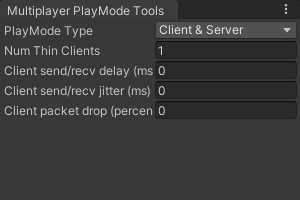
\includegraphics[width=0.50\columnwidth]{gfx/imgs/chapter3/MultiplayerPlayModeTools.png}
    \caption{Finestra \emph{Multiplayer PlayMode Tools}.}
    \label{fig:multiplayer-playmode-tools}
\end{figure}

\subsection{Stabilire una connessione}
\label{subsec:netcode-stabilire-connessione}
La connessione alla rete utilizza il Transport package ed immagazzina le connessioni come entità. Ogni entità connessione presenta un componente \verb|NetworkStreamConnection| che contiene una struttura \verb|NetworkConnection|.
Affinché la comunicazione venga avviata ed il server possa iniziare ad inviare snapshot ai client (ovvero gli stati del gioco), dopo aver ottenuto un riferimento a \verb|NetworkStreamReceiveSystem|, è necessario che:
\begin{enumerate}
    \item Il server entri in stato listening per ricevere richieste di connessione su una porta, chiamando il metodo \verb|Listen()| sul sistema.
    \item Un client si connetta al server, chiamando il metodo \verb|Connect()| sul sistema (a questo punto client e server sono connessi tramite una socket UDP).
    \item Il server marchi tutte le connessioni come ``in gioco'', tramite il componente \verb|NetworkStreamInGame| (ora client e server possono comunicare tramite comandi e snapshot)~\cite{doc:unity-netcode-manual}.
\end{enumerate}

Per richiedere una disconnessione è necessario aggiungere un componente \verb|NetworkStreamRequestDisconnect| all'entità che rappresenta la connessione. Dopodiché a questa viene aggiunto il componente \verb|NetworkStreamDisconnect| per un frame ed infine avviene effettivamente la disconnessione (l'entità viene eliminata)~\cite{youtube:unity-netcode}.

\begin{lstlisting}[caption={Prototipo: stabilimento della connessione.}, label={lst:example-connection},language={[Sharp]C}]
#region Stabilimento connessione

// itera su tutti i mondi presenti
foreach (var world in World.All) 
{
    var network = world.GetExistingSystem<NetworkStreamReceiveSystem>();
    // Codice eseguito nel caso ci troviamo in ClientWorld#
    if (world.GetExistingSystem<ClientSimulationSystemGroup>() != null) 
    {
        world.EntityManager.CreateEntity(typeof(EnableGame));
        NetworkEndPoint ep = NetworkEndPoint.LoopbackIpv4;
        ep.Port = 7979;
        network.Connect(ep); // Connect
    }
    // Codice eseguito nel caso ci troviamo in ServerWorld
    else if (world.GetExistingSystem<ServerSimulationSystemGroup>() != null) 
    {
        world.EntityManager.CreateEntity(typeof(EnableGame));
        NetworkEndPoint ep = NetworkEndPoint.AnyIpv4;
        ep.Port = 7979;
        network.Listen(ep); // Listen
    }
}

#endregion
\end{lstlisting}

\subsection{Comunicazione in NetCode}
Dopo aver stabilito la connessione, è possibile far comunicare i client ed il server. In NetCode esistono principalmente tre modi per comunicare, tramite RPC, comandi oppure snapshot.

\subsubsection{Comunicazione tramite RPC}
\label{subsubsec:comunicazione-rpc}
In NetCode è possibile utilizzare le RPC basandosi sul modello di ECS. Per creare una RPC in NetCode è necessario creare un comando (eventualmente contenente dei campi, rigorosamente di tipo blittable), implementando l'interfaccia \verb|IRpcCommand|. Questa interfaccia estende semplicemente \verb|IComponentData|, senza aggiungervi nulla, ma serve per indicare a NetCode che si riferisce ad un comando RPC.

\begin{lstlisting}[caption={Esempio di comando RPC non contenente campi.}, label={lst:example-rpc-struct},language={[Sharp]C}]
public struct OurRpcCommand : IRpcCommand
{
}
\end{lstlisting}

Implementando questo comando, NetCode genera automaticamente il codice utile per la serializzazione, deserializzazione e registrazione della RPC (in caso fosse necessario è possibile implementarlo manualmente).

Poiché NetCode si basa su ECS, per utilizzare le RPC è necessario creare un'entità che invii il comando ed una che lo riceva. Ciò viene realizzato creando un'entità mittente e aggiungendovi il comando creato ed un componente \verb|SendRpcCommandRequestComponent|, il quale contiene una struttura \verb|NetworkConnection| relativa al destinatario. Nel caso del client non è necessario indicare a chi è diretta, in quanto l'unico endpoint con cui può comunicare è il server a cui è connesso. Al contrario, se il server volesse inviare una richiesta di RPC, dovrebbe specificare a quale connessione questa è diretta e, in caso venga impostata a \verb|Entity.Null|, il messaggio verrebbe inviato in broadcast a tutti i client connessi. Solitamente quanto descritto viene inserito nel codice della \verb|OnUpdate()| di un sistema.

\begin{lstlisting}[caption={Esempio di invio di un comando Rpc dal client.}, label={lst:example-rpc-client-system},language={[Sharp]C}]
#region Invio Rpc

var commandBuffer = new EntityCommandBuffer(Allocator.Temp);
var req = commandBuffer.CreateEntity();

// aggiunge il componente del comando RPC creato in precedenza
commandBuffer.AddComponent(req, new OurRpcCommand());

// indica a NetCode che vogliamo inviare la RPC al server
commandBuffer.AddComponent(req, new SendRpcCommandRequestComponent());
commandBuffer.Playback(EntityManager);

#endregion
\end{lstlisting}

Ciò che non vediamo è che nei world di client e server è presente un sistema \verb|RpcSystem| che rileva l'invio e la ricezione di richieste RPC: appena viene aggiunto il componente \verb|SendRpcCommandRequestComponent| ad un'entità, tale sistema invia la richiesta ed elimina l'entità nel mondo in cui è stata creata; sul lato del destinatario, invece, \verb|RpcSystem| crea un'entità con lo stesso comando \verb|IRpcCommand| ed un componente \verb|ReceiveRpcCommandRequestComponent|~\cite{doc:unity-netcode-manual}. A tal proposito, per rilevare la ricezione di una RPC in un sistema, possiamo iterare su tutte le entità che possiedono quel componente ed eliminarle una volta processati i dati, come vediamo in Codice~\ref{lst:example-rpc-server-system}.

\begin{lstlisting}[caption={Esempio di ricezione di un comando Rpc sul server.}, label={lst:example-rpc-server-system},language={[Sharp]C}]
#region Ricezione Rpc

var commandBuffer = new EntityCommandBuffer(Allocator.Temp);

// itera su tutte le entita' che hanno il comando Rpc creato ed il componente che
// indica la ricezione, il quale permette anche di capire quale client l'ha inviato.
Entities.ForEach((Entity entity, ref OurRpcCommand cmd,
    ref ReceiveRpcCommandRequestComponent req) => {
    
    // una volta ricevuta l'entita' dobbiamo distruggerla, altrimenti
    // l'espressione della lambda continua a fare match con lo stesso comando Rpc. 
    PostUpdateCommands.DestroyEntity(entity);
    
    // [...]
}).Run();
commandBuffer.Playback(EntityManager);

#endregion
\end{lstlisting}

\subsubsection{Stream di comandi}
I client inviano continuamente uno stream di comandi al server (che li riceve in un buffer specifico), che includono tutti gli input e gli ACK dell'ultima snapshot ricevuta. NetCode utilizza il sistema \verb|NullCommandSendSystem| per inviare ACK anche nel caso non vengano ricevuti nuovi comandi, così da mantenere attivo il flusso della comunicazione.

Per creare un nuovo tipo di comando è possibile implementare l'interfaccia \verb|ICommandData|, che eredita da \verb|IBufferElementData|, al cui interno è necessario fornire una proprietà per accedere al \verb|Tick|~\cite{doc:unity-netcode-api}.

\begin{lstlisting}[caption={Prototipo(client): comando per l'input del giocatore.}, label={lst:example-command-data},language={[Sharp]C}]
public struct PlayerInput : ICommandData
{
    public uint Tick { get; set; }
    public int horizontal;
    public int vertical;
}
\end{lstlisting}

Come per le RPC il codice per la serializzazione e deserializzazione viene generato automaticamente se non specificato manualmente.

Una volta creato il comando, è possibile creare un sistema che campioni gli input del giocatore, e li invii al server, appunto, sotto forma di comandi. Per fare ciò è necessario che gli input vengano accumulati in un buffer, prima di poter essere inviati al server, pertanto bisogna aggiungere un buffer, del nuovo tipo di comando creato, all'entità del giocatore (che può essere, ad esempio, il suo personaggio). Dopodiché, è necessario aggiungere il componente \verb|CommandTargetComponent| all'entità che rappresenta la connessione. Così è possibile fare in modo che il \verb|CommandTargetComponent| referenzi l'entità del giocatore, a cui è stato aggiunto il buffer per i comandi.

Quando si aggiungono comandi al buffer, è necessario aggiornare anche il valore di \verb|Tick|, con il valore di \verb|ServerTick|, ottenuto da \verb|ClientSimulationSystemGroup|. In questo modo il server potrà applicare l'input nel momento giusto alla simulazione e inviare
al client una snapshot corretta~\cite{doc:unity-netcode-manual}.

\begin{lstlisting}[caption={Prototipo(client): parte del sistema che campiona gli input del giocatore e li invia al server sotto forma di comandi.}, label={lst:example-command-input},language={[Sharp]C}]
#region Rilevazione input e Invio del comando al server

var localInput = GetSingleton<CommandTargetComponent>().targetEntity;

// [...]

var input = default(PlayerInput);
input.Tick = m_ClientSimulationSystemGroup.ServerTick;

// input del giocatore e aggiornamento del valore del comando
if (Input.GetKey("a"))
    input.horizontal -= 1;
if (Input.GetKey("d"))
    input.horizontal += 1;
if (Input.GetKey("s"))
    input.vertical -= 1;
if (Input.GetKey("w"))
    input.vertical += 1;

// aggiunta del comando al buffer
var inputBuffer = EntityManager.GetBuffer<PlayerInput>(localInput);
inputBuffer.AddCommandData(input);

#endregion
\end{lstlisting}

Per accedere agli input ricevuti dal client, è possibile creare un sistema lato server, che legga tali valori da un'entità contenente il buffer di comandi. La lettura dev'essere effettuata assolutamente tramite il metodo \verb|GetDataAtTick()| del buffer, che permette di ottenere il tick esatto in cui è stato inserito l'input dal client, altrimenti le simulazioni non corrisponderebbero e il gioco potrebbe comportarsi in modi imprevisti.

\begin{lstlisting}[caption={Prototipo(server): parte della lambda expression che aggiorna la velocità del personaggio del giocatore, all'interno del sistema che riceve i comandi.}, label={lst:example-command-output},language={[Sharp]C}]
#region Applicazione del comando al personaggio

PlayerInput input;
inputBuffer.GetDataAtTick(tick, out input);
var speed = pms.speed;

// aggiorna la velocita' del personaggio del giocatore
if (input.horizontal > 0)
    pv.Linear.x += speed * deltaTime;
if (input.horizontal < 0)
    pv.Linear.x -= speed * deltaTime;
if (input.vertical > 0)
    pv.Linear.z += speed * deltaTime;
if (input.vertical < 0)
    pv.Linear.z -= speed * deltaTime;
    
#endregion
\end{lstlisting}

Nel caso per la comunicazione fosse necessario inviare uno stream costante di dati da client a server, si consiglia di utilizzare \verb|ICommandData|, piuttosto che \verb|IRpcCommand|~\cite{doc:unity-netcode-api}. % API ICommandData - utilissimo

\subsubsection{Ghost snapshot}
Il sistema di ghost snapshot di NetCode invia aggiornamenti sullo stato di gioco sincronizzando le entità che esistono sul server, marcate come ghost, con tutti i client. Il server processa per chunk, mentre i client (coloro che ricevono le snapshot), processano per entità. Questo perché non è possibile processare per chunk su entrambi i lati ed il server necessità di un processamento più efficiente, in quanto mantiene più connessioni del client.

Il componente \verb|GhostAuthoringComponent| permette di modificare le impostazioni dei vari ghost, indicando se supporta l'interpolazione, la predizione o entrambe, e se dev'essere sempre interpolato, se vi dev'essere applicata la predizione di tutti o solo del client a cui appartiene. Quest'ultima opzione indica che in tutti i client a cui non appartiene il ghost esso verrà interpolato e, per essere applicata, necessita anche dell'aggiunta del componente \verb|GhostOwnerComponentAuthoring|, il cui campo \verb|NetworkId| dev'essere impostato dal codice per impostarne il proprietario.

\subsection{Predizione lato client}
Per implementare la predizione in un gioco multiplayer, il client deve eseguire la stessa simulazione del server. Così facendo, il client può applicare gli input direttamente al personaggio locale, riducendo notevolmente la latenza, e ricevere snapshot dal server per controllare che la simulazione sia corretta.

NetCode applica la predizione a tutte le entità che a tempo di esecuzione hanno il componente \verb|PredictedGhostComponent|. Questo componente viene aggiunto, dal sistema di conversione dei ghost \verb|GhostAuthoringConversion|, a tutti i ghost con la predizione abilitata sul client e a tutti i ghost, senza distinzione, sul server. Questo perché non serve predire un ghost interpolato se i dati vengono utilizzati solo dal client.
\verb|PredictedGhostComponent| contiene, lato client, informazioni sulla predizione, fra cui ad esempio quali snapshot sono state applicate al ghost.

Per applicare la predizione in un sistema è necessario aggiungere l'attributo \verb|[UpdateInGroup(typeof(GhostPredictionSystemGroup))]|. Questo gruppo esegue sempre ad un timestep fisso, per ottenere gli stessi risultati su client e server.

Poiché il ciclo di predizione esegue dall'ultimo tick applicato ad ogni entità e alcune potrebbero avere già nuovi dati, sul client è necessario controllare se queste devono essere simulate oppure no, utilizzando il metodo \verb|GhostPredictionSystemGroup.ShouldPredict()| prima di aggiornare un'entità: se restituisse un valore falso, il codice dell'aggiornamento non dovrebbe essere eseguito per tale entità.

Il ciclo di predizione del server esegue esattamente una sola volta, e non aggiorna la struttura \verb|TimeData| in quanto è già corretta. Ciononostante, imposta comunque \verb|GhostPredictionSystemGroup.PredictingTick| per assicurare che lo stesso esatto codice possa essere eseguito sia lato client che lato server.

\subsection{Sincronizzazione del tempo}
Poiché NetCode utilizza un modello a server autoritativo, il server esegue ad un timestep fisso basato su quanto tempo è passato dall'ultimo aggiornamento, mentre il client, ad eccezione del codice di predizione che esegue anch'esso sempre ad un timestep fisso, aggiorna ad un timestep dinamico. Affinché il modello funzioni, il client deve far corrispondere ogni volta il proprio tempo a quello del server.

A tal proposito il sistema \verb|NetworkTimeSystem| calcola quale tempo del server dev'essere presentato sul client, facendo una stima iniziale in base al RTT e all'ultima snapshot ricevuta dal client. Quando il client riceve una stima iniziale, apporta piccoli cambiamenti al tempo corrente, basandosi sul tempo trascorso da quanto arrivano i comandi sul server e quando vengono effettivamente utilizzati: ricevendo questo valore dal server, il client può aggiustare il proprio tempo in modo tale da ricevere aggiornamenti appena prima che gli servano.

In altre parole, quando il client invia dei comandi al server, questi arriveranno ad un certo punto in futuro. Quando il server li riceve, li applica alla simulazione, ma il client deve poter stimare a quale tick questo avverrà sul server, così da poter applicare anche lui l'input nello stesso momento della simulazione. A tal proposito, il client fa una stima del \emph{prediction tick}, ovvero il tick in cui il server applicherà i comandi nella sua simulazione (quella corretta), riuscendo ad ottenere un'approssimazione notevole.

Per gli oggetti interpolati il funzionamento è diverso: il client dovrebbe presentarli in uno stato per cui ne ha ricevuto i dati. Questo tempo viene chiamato \emph{interpolazione} e Unity lo calcola inserendo un offset al tempo di predizione. L'offset, chiamato \emph{interpolation delay}, viene aggiustato tramite piccoli incrementi e decrementi, per fare in modo che il tempo di interpolazione avanzi in modo fluido. Unity calcola l'interpolation delay in base al RTT ed al jitter in modo tale che questo dato sia generalmente sempre disponibile e, poiché il tempo aggiunto è basato sul tick rate della rete, è anche robusto ad eventuali perdite di pacchetti.
       % 3.Unity NetCode
\cleardoublepage

\chapter{Unity DOTS: Sviluppo del Prototipo}
\label{cap:prototipo}

Al fine di fornire una dimostrazione pratica dell'utilizzo dell'architettura Unity DOTS, abbiamo realizzato il seguente prototipo, che consiste in un piccolo gioco multigiocatore. L'obbiettivo del progetto è quello di realizzare un gameplay basilare, con movimento dei personaggi e piccole interazioni con l'ambiente di gioco, ad esempio la raccolta degli oggetti di scena. In particolare, ogni giocatore controlla il proprio ``CapsulePlayer'' e può interagire con gli oggetti di scena grazie al sistema di collisione e trigger fornito dal package Physics. La trattazione di quest'ultimo esula dall'argomento della tesi, per cui si rimanda alla documentazione ufficiale disponibile a~\cite{doc:unity-physics-manual}.

\begin{figure}[!ht]
    \centering
    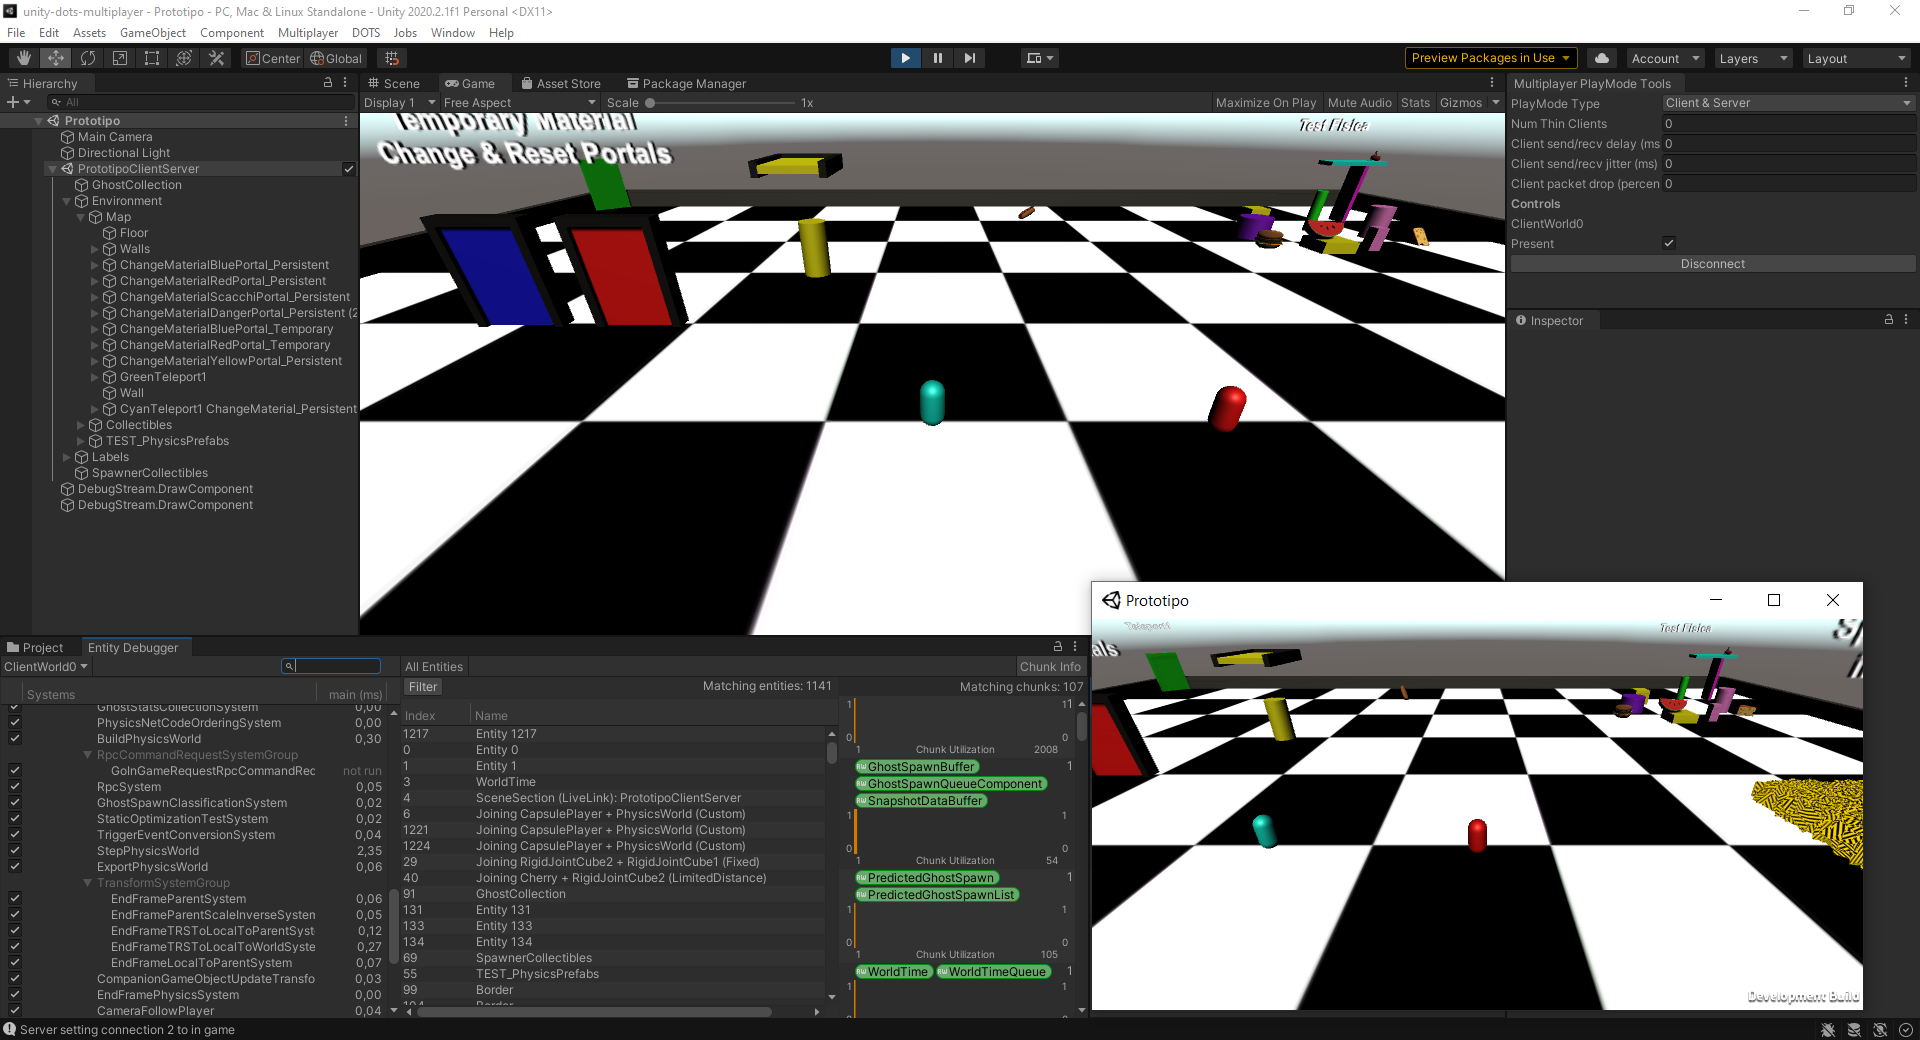
\includegraphics[width=0.95\columnwidth]{gfx/imgs/chapter4/ShowcasePrototipo.png}
    \caption{Prototipo Unity DOTS.}
    \label{fig:prototipo-dots}
\end{figure}

\section{Funzionalità}
Il prototipo permette di avviare un server in ascolto sulla porta 7979, e al quale i client possono connettersi. Una volta stabilita la connessione, il server fa entrare in gioco i client e per ciascuno di essi crea un personaggio capsula all'interno della scena. Da questo momento i vari giocatori possono iniziare a muoversi all'interno della mappa di gioco, interagendo con i molteplici oggetti di scena. In particolare, sono presenti:

\begin{itemize}
    \item Portali che cambiano il materiale di ciò che li attraversa in modo temporaneo o permanente.
    \item Teletrasporti.
    \item Oggetti di varie forme, dimensioni e proprietà fisiche.
    \item Oggetti raccoglibili e che incrementano il punteggio del giocatore.
\end{itemize}

\section{Sviluppo e implementazione}

Il prototipo è stato realizzato utilizzando Unity2020.2.1f1. Abbiamo creato un progetto 3D vuoto e, oltre ai package di default di Unity, vi abbiamo aggiunto i seguenti package: \textbf{Entities}, Hybrid Renderer, Platform Windows, \textbf{NetCode}, Transport, Physics.

\begin{figure}[!ht]
    \begin{subfigure}{.49\textwidth}
      \centering
      % include first image
      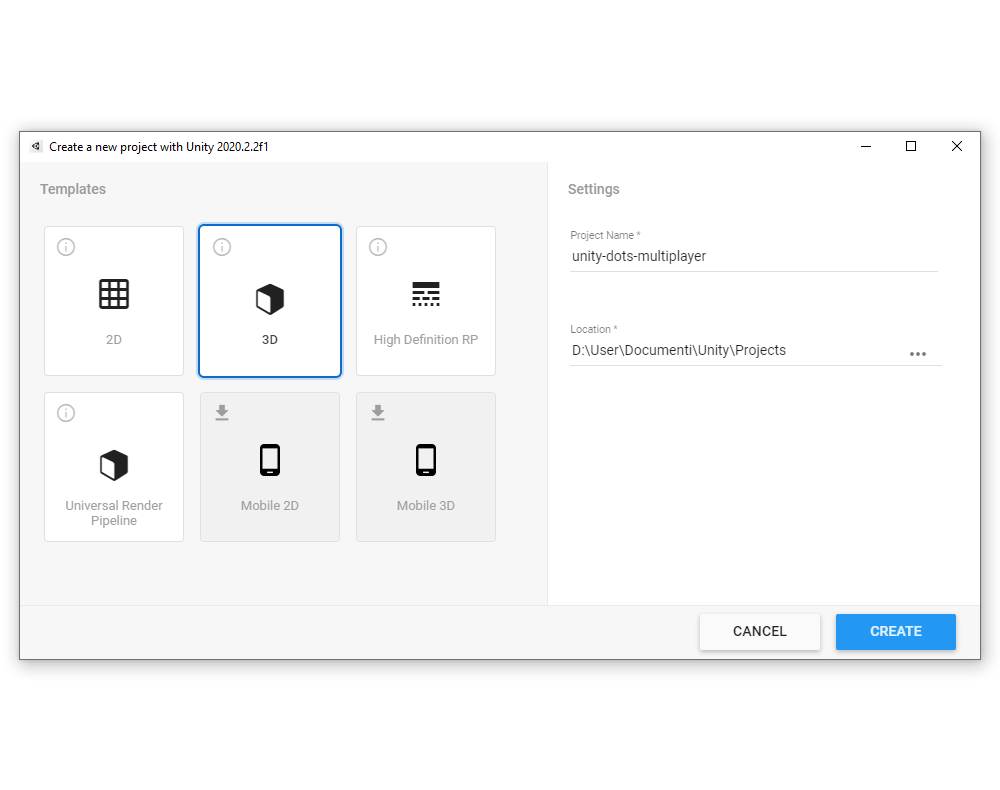
\includegraphics[width=.95\linewidth]{gfx/imgs/chapter4/CreazioneProgetto.png}
      \caption{Creazione progetto.}
      \label{fig:prototipo-creazione-progetto}
    \end{subfigure}
    \begin{subfigure}{.49\textwidth}
      \centering
      % include second image
      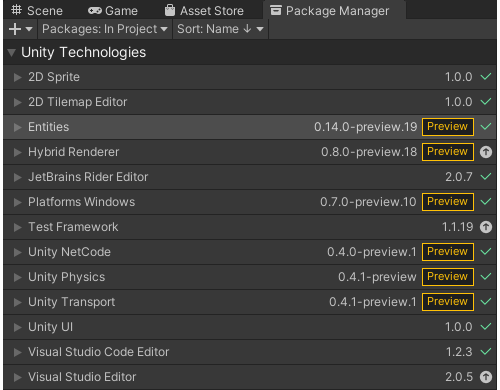
\includegraphics[width=.95\linewidth]{gfx/imgs/chapter4/PackagesPrototipo(actual)2.png}
      \caption{Package Manager.}
      \label{fig:prototipo-packages}
    \end{subfigure}
    \caption{Creazione del progetto e setup.}
    \label{fig:prototipo-setup-progetto}
\end{figure}

Al momento della creazione del prototipo, la maggior parte di questi package vengono forniti attraverso una versione di preview. Di conseguenza, per importarli è stato necessario aprire il pannello \emph{Package Manager} (Figura~\ref{fig:prototipo-packages}) ed inserire l'URL di ognuno dei package manualmente. (Figura~\ref{fig:prototipo-import-packages}). Per ottenere l'URL specifico del package che vogliamo importare, possiamo fare riferimento al manuale ufficiale di Unity~\cite{doc:unity-preview-packages}.


\begin{figure}[!ht]
    \begin{subfigure}{.49\textwidth}
      \centering
      % include first image
      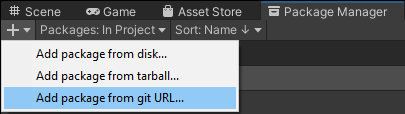
\includegraphics[width=.95\linewidth]{gfx/imgs/chapter4/SetupAddPackageFromURL.png}
      \caption{Aggiunta package tramite URL.}
      \label{fig:prototipo-import1}
    \end{subfigure}
    \begin{subfigure}{.49\textwidth}
      \centering
      % include second image
      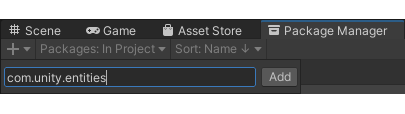
\includegraphics[width=.95\linewidth]{gfx/imgs/chapter4/SetupAddPackageFromURL(2).png}
      \caption{Esempio aggiunta di Entities.}
      \label{fig:prototipo-import2}
    \end{subfigure}
    \caption{Importazione package nel progetto.}
    \label{fig:prototipo-import-packages}
\end{figure}

In alternativa è possibile importare i package aggiungendo gli URL e la relativa versione che si desidera utilizzare, nel file manifest.json, che si trova nella sottodirectory Packages del progetto.

\subsection{Connessione}

Per avviare il gioco possiamo entrare in Play Mode dall'editor Unity, oppure possiamo lanciare una build standalone. Fatto ciò, entra in esecuzione il sistema \verb|Game|. Questo sistema si occupa di stabilire la connessione tra i vari client ed il server; e tramite la chiamata al metodo \verb|RequireSingletonForUpdate| ed il componente \verb|InitGameComponent|, ci assicuriamo che il sistema esegua una sola volta per ogni avvio dell'applicazione.

All'interno di \verb|OnUpdate()| il sistema elimina il componente singleton \verb|InitGameComponent| ed itera su tutti i mondi disponibili (vedi Codice~\ref{lst:prototipo-game-connessione}). Se all'interno di questi è presente il sistema \verb|ClientSimulationSystemGroup| significa che sta eseguendo un client, mentre se vi è \verb|ServerSimulationSystemGroup|, ci si trova nel server. Una volta ottenuto il sistema \verb|NetworkStreamReceiveSystem|, è possibile utilizzarne la classe per mettersi in ascolto delle connessioni su qualsiasi indirizzo (nel nostro caso sulla porta 7979), qualora ci si trovi nel server, oppure connettersi a quest'ultimo nel caso del client.
\SaveVerb{GameTerm}|Game.cs|

\begin{lstlisting}[caption={File \UseVerb{GameTerm}: stabilimento della connessione.}, label={lst:prototipo-game-connessione}, language={[Sharp]C}]
public struct EnableGame : IComponentData
{
}

[UpdateInWorld(UpdateInWorld.TargetWorld.Default)]
[AlwaysSynchronizeSystem]
public class Game : SystemBase
{
    struct InitGameComponent : IComponentData
    {
    }
    protected override void OnCreate()
    {
        RequireSingletonForUpdate<InitGameComponent>();
        EntityManager.CreateEntity(typeof(InitGameComponent));
    }
    protected override void OnUpdate()
    {
        EntityManager.DestroyEntity(GetSingletonEntity<InitGameComponent>());
        foreach (var world in World.All)
        {
            var network = world.GetExistingSystem<NetworkStreamReceiveSystem>();
            if (world.GetExistingSystem<ClientSimulationSystemGroup>() != null)
            {
                world.EntityManager.CreateEntity(typeof(EnableGame));
                NetworkEndPoint ep = NetworkEndPoint.LoopbackIpv4;
                ep.Port = 7979;
                network.Connect(ep); // connect a localhost:7979
            }
            else if (world.GetExistingSystem<ServerSimulationSystemGroup>() != null)
            {
                world.EntityManager.CreateEntity(typeof(EnableGame));
                NetworkEndPoint ep = NetworkEndPoint.AnyIpv4;
                ep.Port = 7979;
                network.Listen(ep);
            }
        }
    }
}
\end{lstlisting}

A questo punto client e server sono connessi. Ora è necessario implementare la logica che permette ai client di entrare in gioco e creare i rispettivi personaggi capsula.
Abbiamo implementato questa meccanica tramite la RPC \verb|GoInGameRequest|: il sistema \verb|GoInGameClientSystem| esegue solo se alla connessione non sia ancora stato associato il componente \verb|NetworkStreamInGame|. In tal caso, iteriamo sulle entità associate ad un \verb|NetworkIdComponent|, ovvero il componente che rappresenta una connessione. Infatti, come spiegato nella Sezione~\ref{subsec:netcode-stabilire-connessione}, per avviare la comunicazione dev'essere presente il componente \verb|NetworkStreamInGame|. In questo modo, il client può iniziare a inviare comandi e ricevere snapshot dal server. Nel caso \verb|NetworkStreamInGame| non sia presente, il sistema \verb|GoInGameClientSystem| invia una richiesta RPC al server, creando un'entità e aggiungendovi i componenti \verb|GoInGameRequest| e \verb|SendRpcCommandRequestComponent|. 

\begin{lstlisting}[caption={File \UseVerb{GameTerm}: richiesta di ingresso in gioco del client.}, label={lst:prototipo-game-start-client}, language={[Sharp]C}]
public struct GoInGameRequest : IRpcCommand
{
}

[UpdateInGroup(typeof(ClientSimulationSystemGroup))]
[AlwaysSynchronizeSystem]
public class GoInGameClientSystem : SystemBase
{
    protected override void OnCreate()
    {
        RequireSingletonForUpdate<EnableGame>();
        RequireForUpdate(GetEntityQuery(ComponentType.ReadOnly<NetworkIdComponent>(),
            ComponentType.Exclude<NetworkStreamInGame>()));
    }
    protected override void OnUpdate()
    {
        var commandBuffer = new EntityCommandBuffer(Allocator.Temp);
        Entities
            .WithNone<NetworkStreamInGame>()
            .ForEach((Entity ent, in NetworkIdComponent id) =>
        {
            commandBuffer.AddComponent<NetworkStreamInGame>(ent);
            var req = commandBuffer.CreateEntity();
            commandBuffer.AddComponent<GoInGameRequest>(req);
            commandBuffer.AddComponent(req, 
                new SendRpcCommandRequestComponent { TargetConnection = ent });
        }).Run();
        commandBuffer.Playback(EntityManager);
        commandBuffer.Dispose();
    }
}
\end{lstlisting}

Lato server, eseguiamo il sistema \verb|GoInGameServerSystem|, il quale si aggiorna solo quando viene rilevata la ricezione di una RPC di tipo \verb|GoInGameRequest|. 

Innanzitutto, il server ottiene un  \verb|GhostPrefabCollectionComponent|, in cui troviamo il prefab della capsula da creare per il giocatore. Come possiamo notare da Codice~\ref{lst:prototipo-game-start-server}, il sistema itera sulla lista dei ghost e prende solo quello con il componente \verb|PlayerMovementSpeed|, ovvero \verb|CapsulePlayer|. A questo punto, iteriamo su tutte le entità che hanno il componente \verb|GoInGameRequest| (la nostra RPC) e \verb|ReceiveRpcCommandRequestComponent|. In questo modo, possiamo ottenere la connessione del client che ha inviato tale richiesta. Così facendo, possiamo non solo far entrare un giocatore in gioco quando viene ricevuta la RPC, ma riusciamo anche ad assegnare al ghost \verb|CapsulePlayer| del client il \verb|NetworkId| relativo. Questo è molto importante perché è ciò che ci permette di distinguere le varie capsule dei giocatori a runtime. Infatti, l'assegnazione del \verb|NetworkId| deve necessariamente avvenire tramite il codice, in quanto a compile time ancora non si conosce a chi apparterrà una certa capsula.

A tal proposito, per realizzare le operazioni relative alla ricezione della RPC, abbiamo sfruttato un \verb|EntityCommandBuffer| (Codice~\ref{lst:prototipo-game-start-server}). In particolare, i passi che dobbiamo eseguire sono:
\begin{enumerate}
    \item Aggiungere il componente \verb|NetworkStreamInGame| alla connessione.
    \item Creare la capsula del giocatore.
    \item Inizializzare il \verb|NetworkId| della capsula del client a cui appartiene.
    \item Aggiungere il buffer \verb|PlayerInput| (che servirà in seguito per accumulare i comandi del giocatore).
    \item Infine, dobbiamo eliminare l'entità relativa alla RPC, altrimenti il \verb|ForEach| eseguirebbe di nuovo.
\end{enumerate}

\begin{lstlisting}[caption={File \UseVerb{GameTerm}: ricezione della RPC e avvio della comunicazione con il server, tramite stream di comandi e snapshot.}, label={lst:prototipo-game-start-server}, language={[Sharp]C}]
[UpdateInGroup(typeof(ServerSimulationSystemGroup))]
[AlwaysSynchronizeSystem]
public class GoInGameServerSystem : SystemBase
{
    protected override void OnCreate()
    {
        RequireSingletonForUpdate<EnableGame>();
        RequireForUpdate(GetEntityQuery(ComponentType.ReadOnly<GoInGameRequest>(), ComponentType.ReadOnly<ReceiveRpcCommandRequestComponent>()));
    }
    protected override void OnUpdate()
    {
        var ghostCollection = GetSingletonEntity<GhostPrefabCollectionComponent>();
        var prefab = Entity.Null;
        var prefabs = EntityManager.GetBuffer<GhostPrefabBuffer>(ghostCollection);
        for (int ghostId = 0; ghostId < prefabs.Length; ++ghostId)
        {
            if (EntityManager.HasComponent<PlayerMovementSpeed>(
                prefabs[ghostId].Value))
                prefab = prefabs[ghostId].Value;
        }

        var commandBuffer = new EntityCommandBuffer(Allocator.Temp);
        var networkIdFromEntity = GetComponentDataFromEntity<NetworkIdComponent>(true);
        Entities
            .WithReadOnly(networkIdFromEntity)
            .ForEach((Entity reqEnt, in GoInGameRequest req, 
                in ReceiveRpcCommandRequestComponent reqSrc) =>
        {
            // da qui in poi sara' possibile inviare comandi e ricevere snapshot
            commandBuffer.AddComponent<NetworkStreamInGame>(reqSrc.SourceConnection);
            UnityEngine.Debug.Log(String.Format("Server setting connection {0} to in game", networkIdFromEntity[reqSrc.SourceConnection].Value));

			// spawn della capsula e aggiornamento dell'ID del ghost
            var player = commandBuffer.Instantiate(prefab);
            commandBuffer.SetComponent(player, new GhostOwnerComponent { 
                NetworkId = networkIdFromEntity[reqSrc.SourceConnection].Value });

            commandBuffer.AddBuffer<PlayerInput>(player);
            commandBuffer.SetComponent(reqSrc.SourceConnection, 
                new CommandTargetComponent { targetEntity = player });

            commandBuffer.DestroyEntity(reqEnt);
        }).Run();
        commandBuffer.Playback(EntityManager);
        commandBuffer.Dispose();
    }
}
\end{lstlisting}

Per far sì che questo funzioni, come spiegato nella Sezione~\ref{subsubsec:comunicazione-rpc}, nei mondi di client e server esegue il sistema \verb|RpcSystem|. Questo si occupa della serializzazione e deserializzazione delle RPC. Inoltre, il \verb|RpcSystem| svolge due importanti funzioni: lato mittente elimina l'entità relativa alla RPC, mentre lato destinatario aggiunge il componente \verb|ReceiveRpcCommandRequestComponent|.

\begin{figure}[!ht]
    \begin{subfigure}{.54\textwidth}
      \centering
      % include first image
      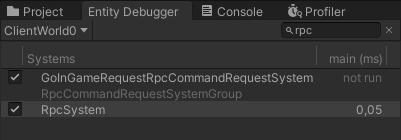
\includegraphics[width=.95\linewidth]{gfx/imgs/chapter4/RpcSystemClient.png}
      \caption{Client.}
      \label{fig:rpc-system-client}
    \end{subfigure}
    \begin{subfigure}{.45\textwidth}
      \centering
      % include second image
      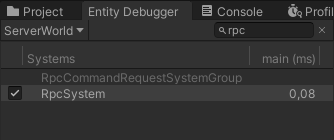
\includegraphics[width=.95\linewidth]{gfx/imgs/chapter4/RpcSystemServer.png}
      \caption{Server.}
      \label{fig:rpc-system-server}
    \end{subfigure}
    \caption{RpcSystem in esecuzione su client e server.}
    \label{fig:rpc-system}
\end{figure}

\subsection{Comunicazione}
Ora che le connessioni sono state marcate come ``in gioco'', client e server possono comunicare tramite stream di comandi e snapshot. In particolare, il client invia i comandi relativi al movimento della propria capsula, ed il server manda continuamente uno stream di snapshot riguardo lo stato di gioco dei vari ghost.

\subsubsection{Input giocatore}

\SaveVerb{CommandTargetComponentTerm}|CommandTargetComponent|
Come spiegato nel Capitolo~\ref{cap:netcode}, per poter inviare dei comandi è necessario creare una struttura di tipo \verb|ICommandData|, che implementa la proprietà \verb|Tick|. Nel nostro caso (Codice~\ref{lst:prototipo-input-client}) \verb|PlayerInput| contiene i campi \verb|horizontal| e \verb|vertical|. Questi ultimi rappresentano il segno che assumerà il valore della velocità della capsula sugli assi X e Z.

Lato client, la raccolta degli input del giocatore avviene tramite il sistema \verb|PlayerInputSystem|. All'interno di questo sistema, nel metodo \verb|OnUpdate()|, come prima cosa verifichiamo che il singleton \verb|CommandTargetComponent|\footnote{\UseVerb{CommandTargetComponentTerm} è un singleton, diverso per ogni client, che contiene il riferimento all'entità su cui verranno applicati i comandi, ovvero l'unica appartenente al giocatore. Nel nostro caso è la capsula.} contenga il riferimento all'entità associata alla capsula. 
Se il riferimento risulta essere nullo, significa che ci troviamo nella prima esecuzione del sistema. Di conseguenza, dobbiamo semplicemente trovare la capsula che corrisponde al \verb|NetworkId| del giocatore e associarla a \verb|CommandTargetComponent|, perché sicuramente è già stata creata in Codice~\ref{lst:prototipo-game-start-server}.

Dunque, per trovare la nostra capsula iteriamo su tutte le entità che hanno il componente \verb|PlayerMovementSpeed|, ovvero il componente tipico di \verb|CapsulePlayer|. Nei parametri della lambda expression aggiungiamo anche \verb|GhostOwnerComponent|, in quanto contiene il \verb|NetworkId| della capsula, che possiamo usare per ottenere quella appartenente al nostro client. Infatti, confrontando \verb|NetowrkId| con \verb|localPlayerId|, ottenuto dalla connessione, siamo sicuri che la capsula sia quella giusta e possiamo aggiungervi il buffer di comandi.

Una volta certi che \verb|CommandTargetComponent| contenga il riferimento alla capsula del client, possiamo iniziare a campionare gli input del giocatore. Per ogni comando da inviare al server è necessario aggiornare la proprietà \verb|Tick| di \verb|PlayerInput|. In questo modo, quando il server riceverà il comando, saprà a quale tick della sua simulazione applicarlo, per far sì che l'azione avvenga nello stesso momento di quella del client.\\

\SaveVerb{PlayerInputSystemTerm}|PlayerInputSystem.cs|

\begin{lstlisting}[caption={File \UseVerb{PlayerInputSystemTerm}: campionamento degli input del giocatore ed invio al server tramite stream di comandi bufferizzato.}, label={lst:prototipo-input-client}, language={[Sharp]C}]
public struct PlayerInput : ICommandData
{
    public uint Tick { get; set; }
    public int horizontal;
    public int vertical;
}

[UpdateInGroup(typeof(ClientSimulationSystemGroup))]
[AlwaysSynchronizeSystem]
public class PlayerInputSystem : SystemBase
{
    ClientSimulationSystemGroup m_ClientSimulationSystemGroup;
    protected override void OnCreate()
    {
        RequireSingletonForUpdate<NetworkIdComponent>();
        RequireSingletonForUpdate<EnableGame>();
        m_ClientSimulationSystemGroup =
            World.GetExistingSystem<ClientSimulationSystemGroup>();
    }

    protected override void OnUpdate()
    {
        var localInput = GetSingleton<CommandTargetComponent>().targetEntity;
        
		if (localInput == Entity.Null) // riferimento alla capsula assente
        {
			var localPlayerId = GetSingleton<NetworkIdComponent>().Value;
            var commandBuffer = new EntityCommandBuffer(Allocator.Temp);
            var commandTargetEntity = GetSingletonEntity<CommandTargetComponent>();
            
			Entities
			    .WithAll<PlayerMovementSpeed>()
			    .WithNone<PlayerInput>()
			    .ForEach((Entity ent, ref GhostOwnerComponent ghostOwner) =>
            {
				if (ghostOwner.NetworkId == localPlayerId)
                {
                    commandBuffer.AddBuffer<PlayerInput>(ent);
                    commandBuffer.SetComponent(commandTargetEntity, 
                        new CommandTargetComponent { targetEntity = ent });
                }
            }).Run();
            commandBuffer.Playback(EntityManager);
            return;
        }
        
		var input = default(PlayerInput);
		input.Tick = m_ClientSimulationSystemGroup.ServerTick;
        if (Input.GetKey("a"))
            input.horizontal -= 1;
        if (Input.GetKey("d"))
            input.horizontal += 1;
        if (Input.GetKey("s"))
            input.vertical -= 1;
        if (Input.GetKey("w"))
            input.vertical += 1;
        
        var inputBuffer = EntityManager.GetBuffer<PlayerInput>(localInput);
        inputBuffer.AddCommandData(input);
    }
}
\end{lstlisting}

\subsubsection{Movimento capsula}
Una volta che abbiamo campionato gli input possiamo applicarli alla capsula del giocatore. Il sistema che si occupa di questo meccanismo è chiamato  \verb|PlayerMovementSystem|. Possiamo notare come questo esegua all'interno del gruppo \verb|GhostPredictionSystemGroup|, il quale permette di implementare la predizione lato client dei ghost. In particolare, da questo gruppo otteniamo il \verb|PredictionTick|, che possiamo usare per sapere se è necessario eseguire la predizione. In caso negativo viene semplicemente terminata la funzione. Al contrario, in caso affermativo, traduciamo l'input campionato in un movimento. In particolare, aggiorniamo il valore della velocità della capsula e utilizziamo ancora una volta \verb|PredictionTick| per sapere a quale tick è necessario applicarlo.

\SaveVerb{PlayerMovementSystemTerm}|PlayerMovementSystem.cs|

\clearpage
\begin{lstlisting}[caption={File \UseVerb{PlayerMovementSystemTerm}: applicazione del movimento alla capsula, tramite predizione.}, label={lst:prototipo-input-server}, language={[Sharp]C}]
[UpdateInGroup(typeof(GhostPredictionSystemGroup))]
public class PlayerMovementSystem : SystemBase
{
    GhostPredictionSystemGroup m_GhostPredictionSystemGroup;
    protected override void OnCreate()
    {
        m_GhostPredictionSystemGroup =
            World.GetExistingSystem<GhostPredictionSystemGroup>();
    }
    #region Codice Predizione
    
    protected override void OnUpdate() 
    {
        var tick = m_GhostPredictionSystemGroup.PredictingTick;
        var deltaTime = Time.DeltaTime;
        Entities.ForEach((DynamicBuffer<PlayerInput> inputBuffer, 
            ref PhysicsVelocity pv, 
            in PredictedGhostComponent prediction, in PlayerMovementSpeed pms) =>
        {
            if (!GhostPredictionSystemGroup.ShouldPredict(tick, prediction))
                return;
            PlayerInput input;
            inputBuffer.GetDataAtTick(tick, out input);
            var speed = pms.speed;
            
            if (input.horizontal > 0)
                pv.Linear.x += speed * deltaTime;
            if (input.horizontal < 0)
                pv.Linear.x -= speed * deltaTime;
            if (input.vertical > 0)
                pv.Linear.z += speed * deltaTime;
            if (input.vertical < 0)
                pv.Linear.z -= speed * deltaTime;

        }).ScheduleParallel();
    }
    
    #endregion
}
\end{lstlisting}

\subsection{Azioni di gioco}
Oltre al semplice movimento, per rendere il prototipo un po' più interessante, abbiamo realizzato qualche funzionalità aggiuntiva, fra cui la raccolta degli oggetti e qualche portale interattivo.

\subsubsection{Raccolta oggetti}

Per realizzare la meccanica della raccolta degli oggetti, abbiamo innanzitutto creato un componente \verb|CollectibleTagComponent| per marcare le entità che possono essere raccolte.
Dopodiché, sfruttando il package \emph{Physics}, abbiamo implementato un sistema \verb|PickUpSystem| in grado di rilevare le collisioni tra l'entità dell'oggetto e quella di \verb|CapsulePlayer|. Il sistema, appena rileva il trigger della collisione, aggiorna il punteggio del giocatore e aggiunge il componente vuoto \verb|DeleteTagComponent| all'entità dell'oggetto raccoglibile.\\

\begin{lstlisting}[caption={Componente che marca un'entità come raccoglibile.}, label={lst:prototipo-collectible}, language={[Sharp]C}]
[GenerateAuthoringComponent]
public struct CollectibleTagComponent : IComponentData
{
    public float points;
}
\end{lstlisting}

\SaveVerb{PickUpSystemTerm}|PickUpSystem.cs|
\SaveVerb{DeleteTagComponentTerm}|DeleteTagComponent|

\begin{lstlisting}[caption={File \UseVerb{PickUpSystemTerm}: aumento del punteggio del giocatore e aggiunta del tag \UseVerb{DeleteTagComponentTerm} agli oggetti raccoglibili.}, label={lst:prototipo-pickup}, language={[Sharp]C}]
#region Pickup

Entities
    .WithoutBurst()
    .ForEach((Entity e, ref DynamicBuffer<StatefulTriggerEvent> triggerEventBuffer,
        ref CollectibleTagComponent collectibleComponent) =>
{
    for (int i = 0; i < triggerEventBuffer.Length; i++)
    {
        var triggerEvent = triggerEventBuffer[i]; // entita' A
        var otherEntity = triggerEvent.GetOtherEntity(e); // entita' B
        
        // [...]
        
        // quando entra nella hitbox
        if (triggerEvent.State == EventOverlapState.Enter && EntityManager.HasComponent<PlayerMovementSpeed>(otherEntity))
        {
            var punteggioPlayer =
                EntityManager.GetComponentData<PlayerScoreComponent>(otherEntity);
            punteggioPlayer.score += collectibleComponent.points;

            var ghostId =
                EntityManager.GetComponentData<GhostComponent>(otherEntity).ghostId;
            UnityEngine.Debug.Log(String.Format("Il player " + ghostId + 
                " ha raccolto " + collectibleComponent.points + " punti. Tot 
                punti player " + ghostId + ": " + punteggioPlayer.score));

            commandBuffer.SetComponent(otherEntity, punteggioPlayer);
            commandBuffer.AddComponent<DeleteTagComponent>(e, deleteTag);
        }
    }
}).Run();

#endregion
\end{lstlisting}

Il componente \verb|DeleteTagComponent| è un espediente che ci serve per eliminare gli oggetti raccolti: tramite il sistema \verb|DeleteCollectibleSystem| possiamo iterare su tutte le entità marcate da questo componente e rimuoverle.

\begin{lstlisting}[caption={Componente che marca un'entità come ``da eliminare''.}, label={lst:prototipo-delete-tag}, language={[Sharp]C}]
public struct DeleteTagComponent : IComponentData
{
}
\end{lstlisting}

\SaveVerb{DeleteCollectibleSystemTerm}|DeleteCollectibleSystem.cs|
\SaveVerb{DeleteTagComponentTerm}|DeleteTagComponent|

\begin{lstlisting}[caption={File \UseVerb{DeleteCollectibleSystemTerm}: eliminazione delle entità aventi il componente \UseVerb{DeleteTagComponentTerm}.}, label={lst:prototipo-delete-system}, language={[Sharp]C}]
[UpdateInGroup(typeof(ClientAndServerSimulationSystemGroup))]
public class DeleteCollectibleSystem : SystemBase
{
    protected override void OnUpdate()
    {
        EntityCommandBuffer commandBuffer =
            new EntityCommandBuffer(Unity.Collections.Allocator.Temp);

        Entities
            .WithAll<DeleteTagComponent>()
            .ForEach((Entity entity) =>
            {
                commandBuffer.DestroyEntity(entity);
            }).Run();

        commandBuffer.Playback(EntityManager);
        commandBuffer.Dispose();
    }
}
\end{lstlisting}

\begin{figure}[!ht]
    \begin{subfigure}{.49\textwidth}
      \centering
      % include first image
      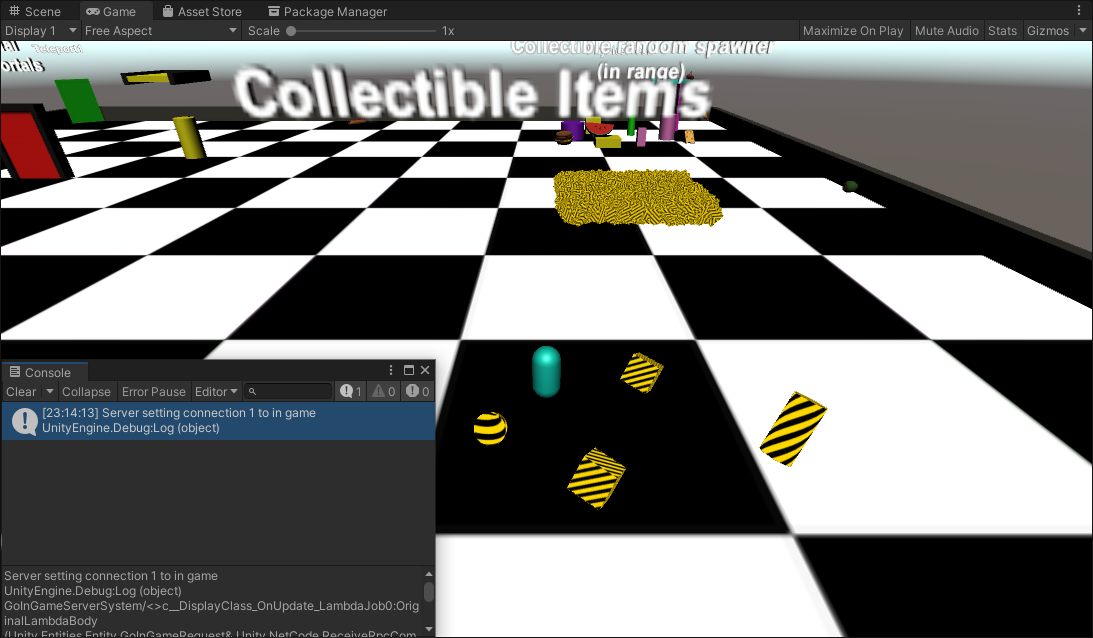
\includegraphics[width=.95\linewidth]{gfx/imgs/chapter4/PickUpCollectible1.png}
      \caption{Prima della raccolta dell'oggetto.}
      \label{fig:pickup-1}
    \end{subfigure}
    \begin{subfigure}{.49\textwidth}
      \centering
      % include second image
      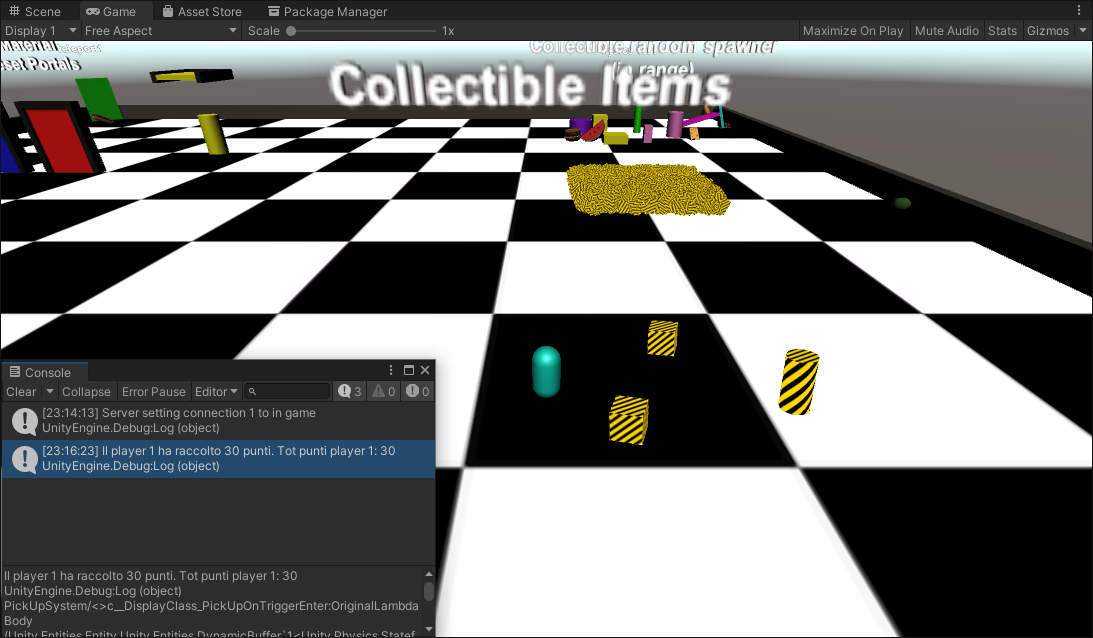
\includegraphics[width=.95\linewidth]{gfx/imgs/chapter4/PickUpCollectible2.png}
      \caption{Dopo la raccolta dell'oggetto.}
      \label{fig:pickup-2}
    \end{subfigure}
    \caption{Raccolta di un oggetto ``Sphere'' e stampa del log del punteggio.}
    \label{fig:pickup-collectibles}
\end{figure}

\subsubsection{Portali cambia-colore}

I portali sono stati realizzati sfruttando lo stesso meccanismo di \verb|PickUpSystem|:
il sistema \verb|PersistentChangeMaterialOnTriggerSystemTerm|, quando rileva il trigger di un'entità che lo attraversa, ne modifica il materiale con quello del portale stesso.

\SaveVerb{PersistentChangeMaterialOnTriggerSystemTerm}|PersistentChangeMaterialOnTriggerSystem.cs|
\SaveVerb{materialTerm}|material|

\begin{lstlisting}[caption={File \UseVerb{PersistentChangeMaterialOnTriggerSystemTerm}: aggiornamento del valore della proprietà \UseVerb{materialTerm} con quello del portale.}, label={lst:prototipo-portal-material}, language={[Sharp]C}]
#region Portale cambia colore

if (triggerEvent.State == EventOverlapState.Enter)
{
    var volumeRenderMesh = EntityManager.GetSharedComponentData<RenderMesh>(e);
    var overlappingRenderMesh = EntityManager.GetSharedComponentData<RenderMesh>(otherEntity);
    overlappingRenderMesh.material = volumeRenderMesh.material;

    commandBuffer.SetSharedComponent(otherEntity, overlappingRenderMesh);
}

#endregion
\end{lstlisting}

\begin{figure}[!ht]
    \begin{subfigure}{.49\textwidth}
      \centering
      % include first image
      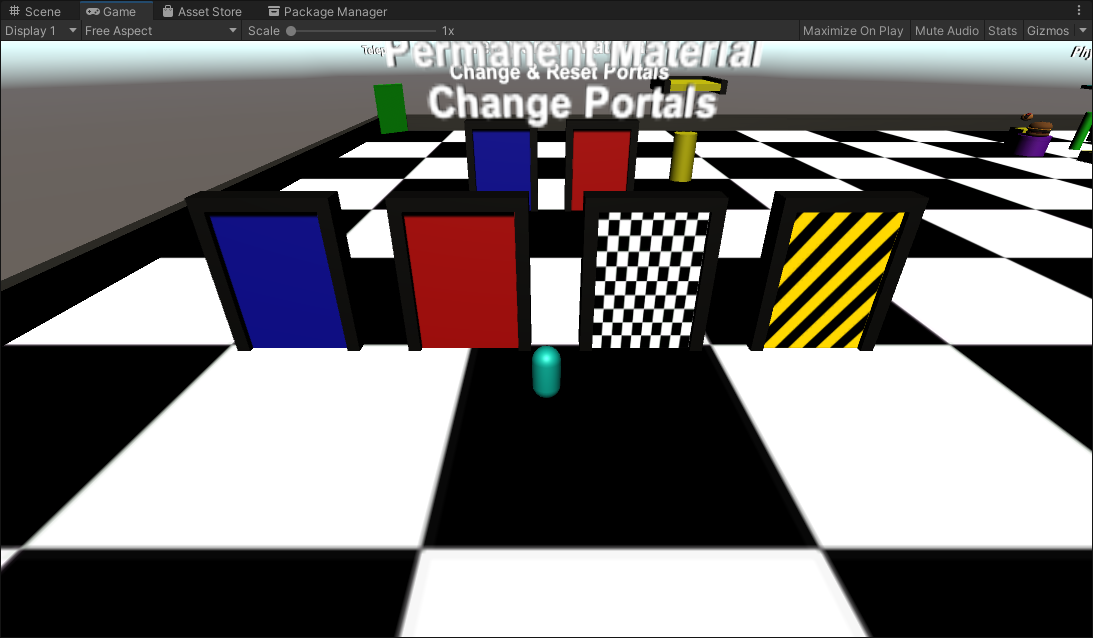
\includegraphics[width=.95\linewidth]{gfx/imgs/chapter4/PortaleCambiaColore1.png}
      \caption{Prima di aver attraversato il portale.}
      \label{fig:portale-colore-1}
    \end{subfigure}
    \begin{subfigure}{.49\textwidth}
      \centering
      % include second image
      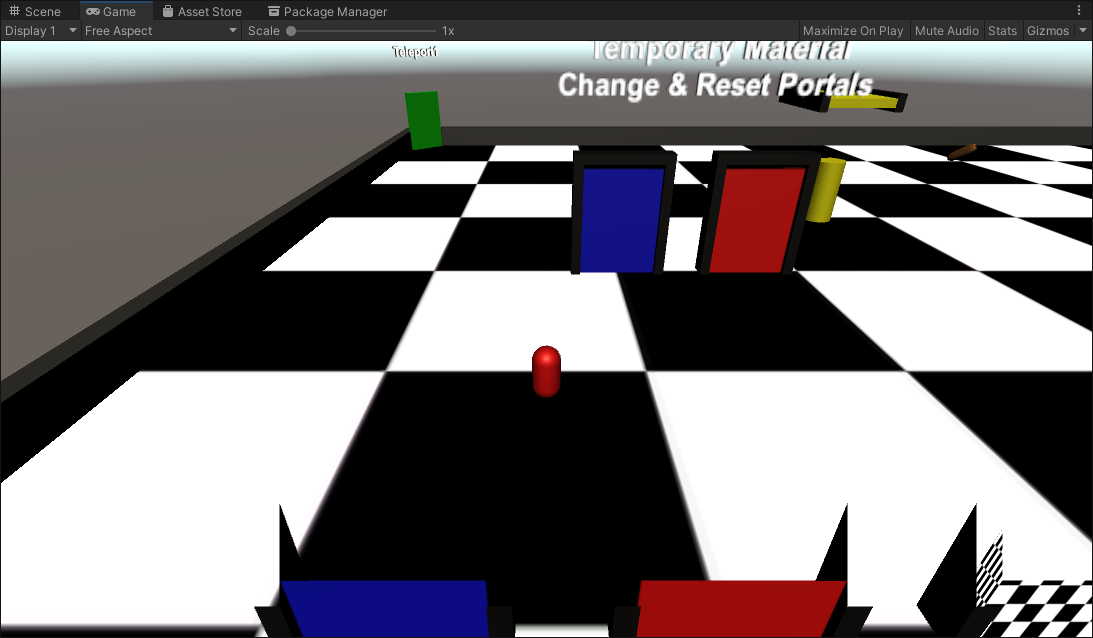
\includegraphics[width=.95\linewidth]{gfx/imgs/chapter4/PortaleCambiaColore2.png}
      \caption{Dopo aver attraversato il portale.}
      \label{fig:portale-colore-2}
    \end{subfigure}
    \caption{Portali cambia-colore (passaggio attraverso il portale rosso).}
    \label{fig:portali-cambia-colore}
\end{figure}

\subsubsection{Camera Follow}
Per rendere l'utilizzo del prototipo più piacevole ed evitare confusione con le varie capsule, abbiamo implementato un meccanismo che permette di ottenere una visuale in terza persona sulla propria entità \verb|CapsulePlayer|.

Il sistema \verb|CameraFollowPlayer| aggiorna la posizione della \verb|camera| principale, spostandola in base al componente \verb|Translation| dell'entità che possiede \verb|PlayerCameraFollowComponent|, ovvero la \verb|CapsulePlayer|. Per muovere solo la capsula del giocatore relativo, come per \verb|PlayerMovementSystem|, abbiamo utilizzato il singleton \verb|CommandTargetComponent|.

\begin{lstlisting}[caption={Componente che permette alla camera di seguire la capsula.}, label={lst:prototipo-camera-follow-component}, language={[Sharp]C}]
[GenerateAuthoringComponent]
public struct PlayerCameraFollowComponent : IComponentData
{
    public float xOffset;
    public float yOffset;
    public float zOffset;
}
\end{lstlisting}

\SaveVerb{CameraFollowPlayerTerm}|CameraFollowPlayer.cs|

\begin{lstlisting}[caption={File \UseVerb{CameraFollowPlayerTerm}: aggiornamento della posizione della camera per seguire la capsula del client.}, label={lst:prototipo-camera-follow-system}, language={[Sharp]C}]
[UpdateInGroup(typeof(ClientSimulationSystemGroup))]
public class CameraFollowPlayer : SystemBase
{
    protected override void OnUpdate()
    {
        var position = Camera.main.transform.position;

        var commandTargetComponentEntity =
            GetSingletonEntity<CommandTargetComponent>();
        var commandTargetComponent =
            GetComponent<CommandTargetComponent>(commandTargetComponentEntity);

        Entities
            .WithAll<PlayerScoreComponent>()
            .ForEach((Entity entity,
                in Translation translation, in PlayerCameraFollowComponent pcf) =>
        {
            // aggiorna solo la posizione rispetto alla propria capsula
            if (entity == commandTargetComponent.targetEntity)
            {
                position.x = translation.Value.x + pcf.xOffset;
                position.y = translation.Value.y + pcf.yOffset;
                position.z = translation.Value.z + pcf.zOffset;
            }
        }).Run();

        Camera.main.transform.position = position;
    }
}
\end{lstlisting}

\subsection{Build standalone}
Ai fini di testing della tesi abbiamo realizzato una sola build standalone per Windows, utilizzando il package \emph{Platforms Windows}. L'applicativo ci permette di eseguire il gioco come client, per cui è necessario avviare anche il server dall'editor Unity per poterlo utilizzare.

\begin{figure}[!ht]
    \begin{subfigure}{.49\textwidth}
      \centering
      % include first image
      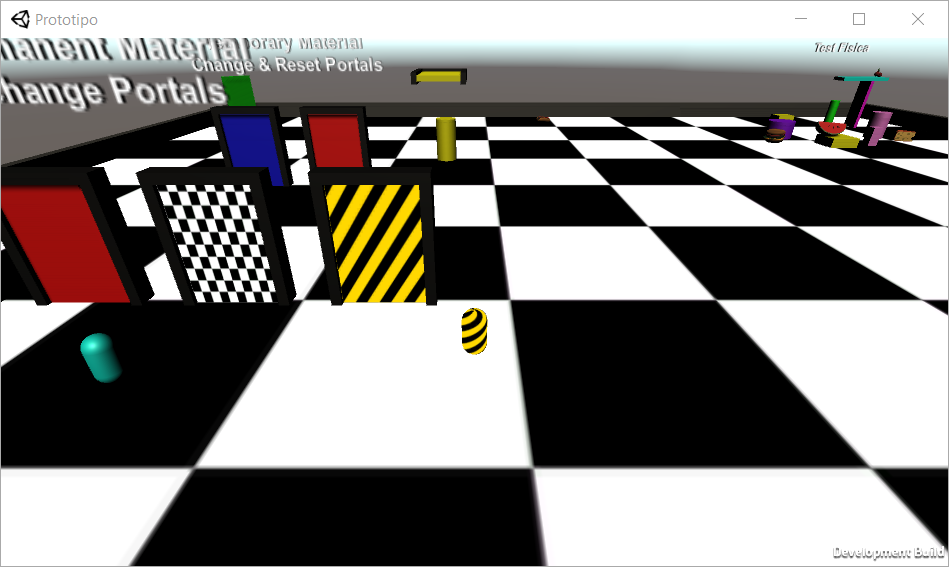
\includegraphics[width=.95\linewidth]{gfx/imgs/chapter4/BuildStandalonePrototipo.png}
      \caption{Build standalone (client).}
      \label{fig:build-standalone}
    \end{subfigure}
    \begin{subfigure}{.49\textwidth}
      \centering
      % include second image
      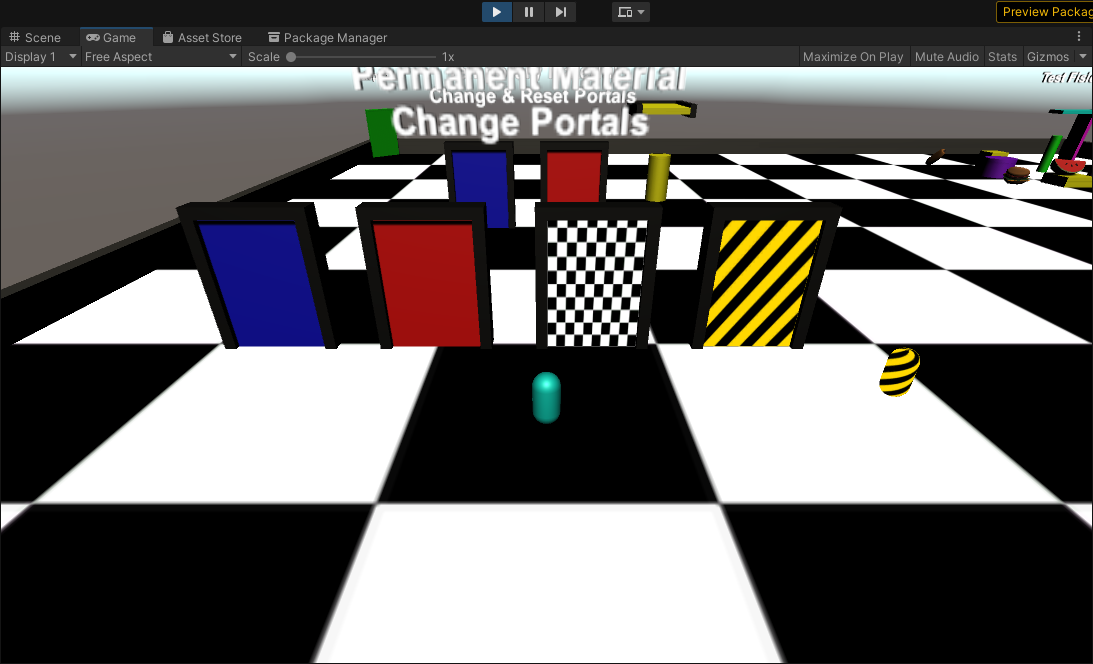
\includegraphics[width=.95\linewidth]{gfx/imgs/chapter4/BuildStandaloneEditor.png}
      \caption{Editor Unity (client \& server).}
      \label{fig:build-editor}
    \end{subfigure}
    \caption{Avvio da Unity in modalità ``Client \& Server'' e connessione dall'applicativo client standalone.}
    \label{fig:build}
\end{figure}
       % 4.Prototipo
\cleardoublepage

\chapter{Risultati Sperimentali}
\label{cap:risultati}

Nel seguente capitolo discuteremo i risultati sperimentali ottenuti con il presente lavoro di tesi.

Nel Capitolo~\ref{cap:prototipo} abbiamo sviluppato un prototipo di videogioco completo basato su Unity DOTS, il quale ci è servito per approfondire le librerie da un punto di vista high-level. In particolare, le funzionalità realizzate lo rendono un progetto completo ed un gioco a tutti gli effetti. Oltre a questo prototipo, per valutare gli aspetti legati alle performance, ne abbiamo sviluppato uno ad hoc per il testing.

Prima di proseguire con l'analisi dei risultati sperimentali, introduciamo alcuni degli strumenti utilizzati per la valutazione.

Lo sviluppo del prototipo ed i relativi test sono stati eseguiti sulla seguente architettura:
\begin{itemize}
    \item Processore Intel(R) Core(TM) i7-7700HQ con 4 core (8 processori logici) e frequenza di clock pari a 2.80GHz.
    \item Memoria RAM da 16GB.
    \item Scheda video NVIDIA GeForce GTX 1060.
    \item Sistema Operativo Microsoft Windows 10 Home, a 64 bit.
\end{itemize}

Per poter analizzare le varie informazioni del sistema, possiamo sfruttare il Profiler Unity (vedi Figura~\ref{fig:prototipo-profiler}. Questo è uno strumento compreso nell'editor, che ci permette esaminare alcuni dei dati pratici: nella parte superiore possiamo vedere il carico sulla CPU dei vari componenti dell'applicazione; nella parte inferiore possiamo vedere dove eseguono effettivamente le parti del nostro codice. Partendo dall'alto verso il basso si costruisce una gerarchia di gruppi e sistemi di esecuzione, dove il più esterno è il ciclo del PlayerLoop, ovvero l'esecuzione dell'applicazione

\begin{figure}[!ht]
    \centering
    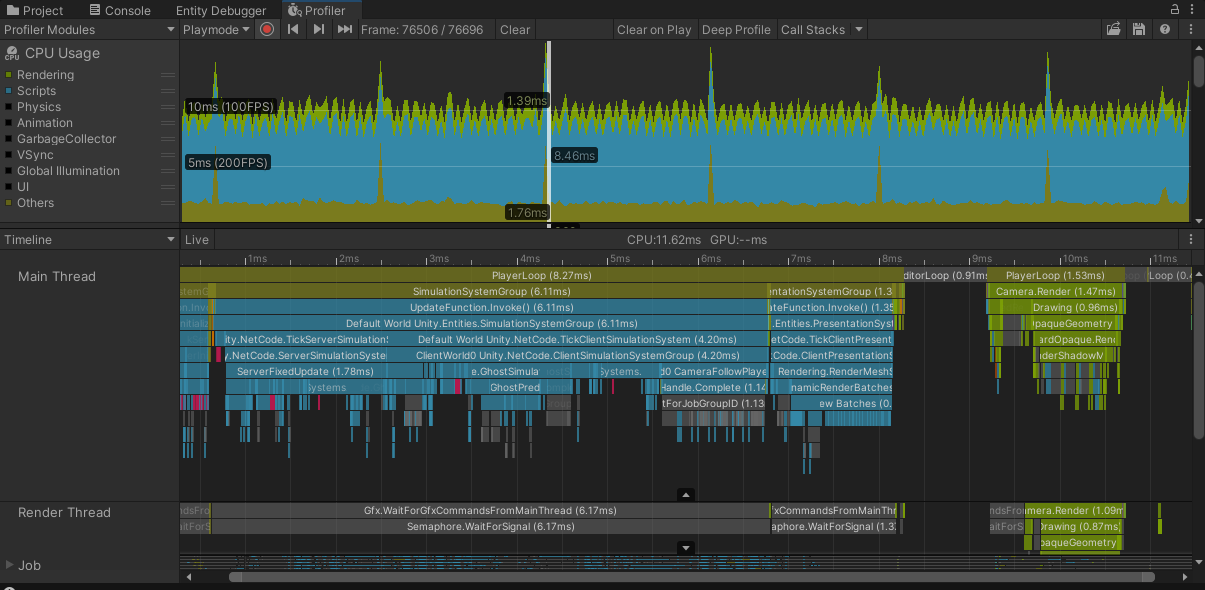
\includegraphics[width=0.95\columnwidth]{gfx/imgs/chapter5/ProfilerPrototipo.png}
    \caption{Profiler Unity: un frame durante l'esecuzione.}
    \label{fig:prototipo-profiler}
\end{figure}


\section{Valutazione performance DOTS}

Per la realizzazione del prototipo sono state costruite due scene, una per il test riguardante l'architettura classica e una per i test relativi ad ECS, Jobs e Burst. In entrambe le scene è presente il medesimo GameObject, il quale è associato ad un componente ``spawner''. Questo componente permette, in base a dei campi modificabili, di creare un numero arbitrario di cubi. Nella prima scena i cubi sono costituiti da GameObject, mentre nella seconda sono costituiti da entità. Gli oggetti creati sono in entrambi i casi dei cubi con una grafica a righe gialle e nere, in modo tale che sia possibile vederne il movimento. Una volta istanziati, i cubi vengono fatti ruotare all'interno della scena. Nel caso dell'architettura classica, la rotazione avviene tramite un MonoBehaviour associato al GameObject del cubo; mentre nel caso di ECS, la rotazione è realizzata da un sistema.

Durante la fase di testing, abbiamo eseguito il prototipo sfruttando diverse configurazioni, ovvero:

\begin{itemize}
    \item Architettura classica, tramite lo spawn di GameObject e rotazione di questi tramite MonoBehaviour.
    \item ECS ``vanilla'', tramite lo spawn di entità e la rotazione di queste aggiornando un sistema sul main thread.
    \item ECS e job, come il precedente ma scheduliamo la \verb|OnUpdate()| del sistema affinché venga eseguita su un singolo worker thread;
    \item ECS e job paralleli, come il precedente, ma scheduliamo diversi job che eseguiranno in parallelo sui worker thread;
    \item ECS e job paralleli, come il precedente ma compilando i job con Burst.
\end{itemize}

La tabella in Figura~\ref{fig:dati-stress-test} riporta i dati rilevati durante le prove:

\begin{figure}[!ht]
    \centering
    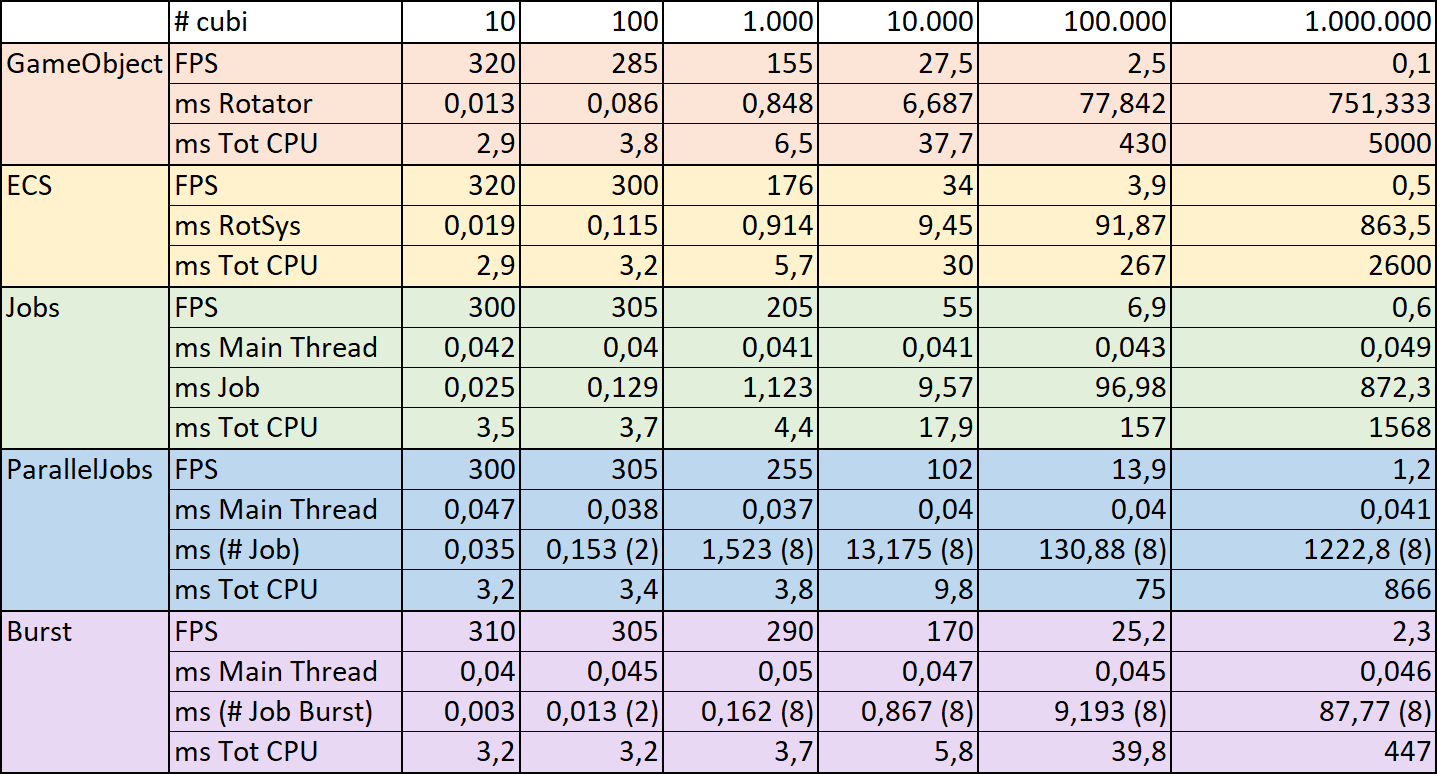
\includegraphics[width=0.95\columnwidth]{gfx/imgs/chapter5/RaccoltaDati.png}
    \caption{Raccolta dati}
    \label{fig:dati-stress-test}
\end{figure}

In particolare, per ogni test abbiamo riportato:
\begin{itemize}
    \item FPS dell'applicazione durante l'esecuzione.
    \item Tempo in millisecondi impiegato dal MonoBehaviour o dai sistemi per ruotare tutti gli oggetti. Nel caso di Jobs, ParallelJobs e Burst, questo valore viene suddiviso fra main thread e worker thread.
    \item Tempo totale in millisecondi impiegato dalla CPU per eseguire un frame completo.
\end{itemize}

Per ottenere i risultati in tabella, abbiamo eseguito il prototipo una volta per ciascuna configurazione. Ad ogni esecuzione abbiamo campionato 10 frame. Dopodiché, per ognuno di questi, abbiamo salvato i valori di FPS e millisecondi, e successivamente calcolato la loro media. Queste operazioni sono poi state ripetute incrementando il numero di cubi creati, come riportato in tabella.

Nelle prossime sezioni approfondiremo i risultati ottenuti per ognuna delle configurazioni testate.

\subsubsection{Architettura classica}
Nel caso dell'architettura classica, vengono prima creati dei GameObject. Successivamente, questi ultimi vengono messi in rotazione per mezzo del MonoBehaviour che posseggono. In particolare, questa rotazione avviene all'interno del metodo \verb|Update()|. Infatti, tramite il profiler possiamo notare come questa funzione venga eseguita per ognuno dei cubi presenti in scena. Sempre grazie al profiler, possiamo vedere come ogni rotazione avvenga in sequenza nel main thread. Se osserviamo il grafico in Figura~\ref{fig:profiler-100k(1)}, vediamo che le 100.000 istanze del MonoBehaviour \verb|Rotator| impiegano circa 76,5 ms per ruotare i GameObject; mentre facendo riferimento alla Figura~\ref{fig:dati-stress-test}, notiamo che l'applicazione viene eseguita con una media di 2,5 FPS.

\begin{figure}[!ht]
    \centering
    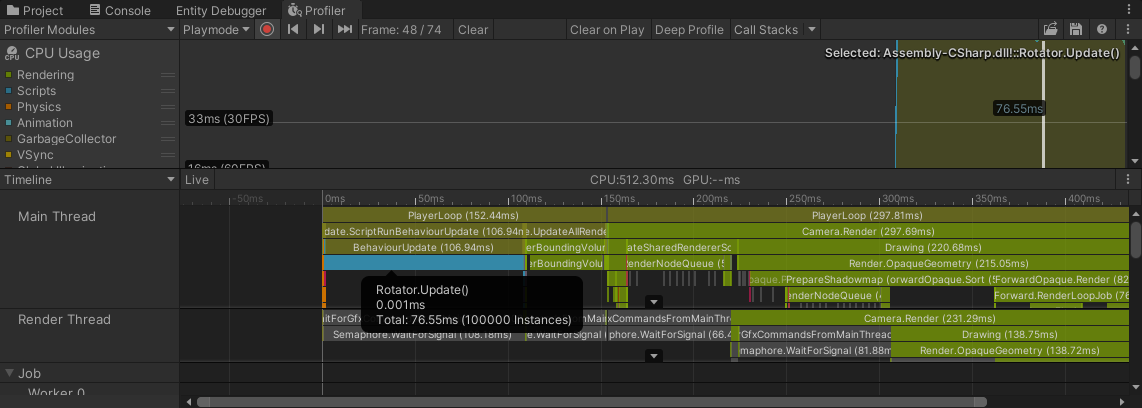
\includegraphics[width=0.95\columnwidth]{gfx/imgs/chapter5/ProfilerStressTest100k(1).png}
    \caption{Profiler: rotazione di 100.000 GameObject tramite un MonoBehaviour.}
    \label{fig:profiler-100k(1)}
\end{figure}

\subsubsection{ECS}
Per i test con ECS abbiamo realizzato un componente \verb|RotateComponent| ed un sistema \verb|RotatorSystem|. Questo componente viene assegnato alle entità dei cubi non appena vengono creati.

Nel test in questione, all'interno del metodo \verb|OnUpdate()| del sistema, eseguiamo la lambda expression che itera sulle entità tramite \verb|Run()|. Così facendo la funzione verrà eseguita sul main thread. Come si può notare in Figura~\ref{fig:profiler-100k(2)}, con 100.000 entità l'esecuzione di \verb|OnUpdate()| all'interno di un singolo frame impiega 89,6 ms. Rispetto al test precedente abbiamo un leggero aumento del tempo impiegato dal solo sistema per svolgere la funzione di rotazione. Tuttavia, dal grafico in Figura~\ref{fig:dati-stress-test} notiamo che l'applicazione esegue a 3,9 FPS, e che quindi, nel complesso, abbiamo ottenuto un miglioramento. Questo comportamento è dovuto al fatto che, anche se il sistema di rotazione impiega più millisecondi della funzione \verb|Update()| del MonoBehaviour, quest'ultima viene chiamata un numero maggiore di volte. Di conseguenza, nel secondo caso abbiamo un tempo di computazione totale più elevato, che si traduce in un numero inferiore di FPS.

\begin{figure}[!ht]
    \centering
    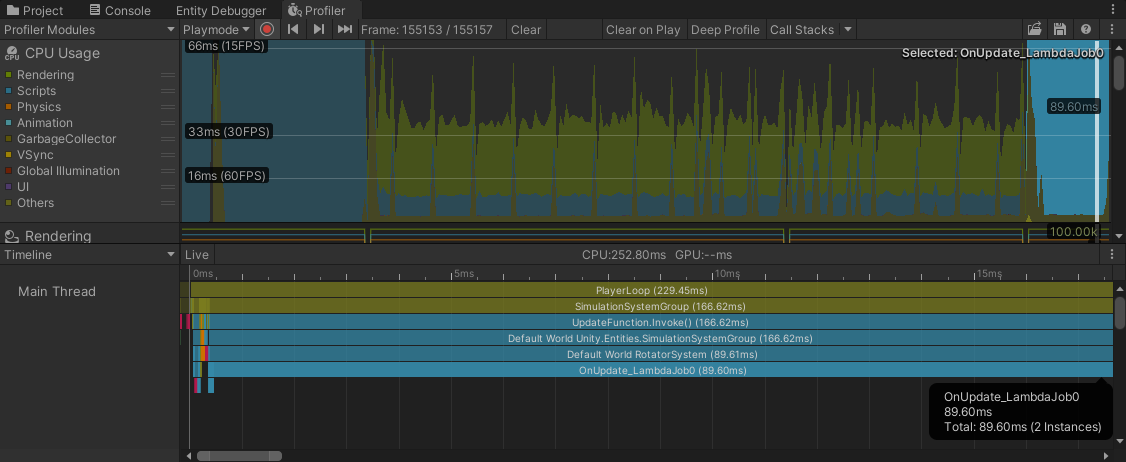
\includegraphics[width=0.95\columnwidth]{gfx/imgs/chapter5/ProfilerStressTest100k(2).png}
    \caption{Profiler: rotazione di 100.000 entità eseguendo il sistema sul main thread.}
    \label{fig:profiler-100k(2)}
\end{figure}

\subsubsection{ECS con job}
In questo test abbiamo utilizzato ECS insieme al Job System. Quindi, invece di eseguire la lambda expression del sistema \verb|RotatorSystem| sul main thread, abbiamo schedulato un job per la sua esecuzione. Così facendo possiamo scaricare il lavoro della CPU su un core secondario.
Dal Profiler possiamo vedere come la \verb|OnUpdate()| sul main thread impieghi solo 0,043 ms, con un notevole miglioramento rispetto alle due prove precedenti. Questo è dovuto al fatto che il lavoro del sistema viene scaricato su un job secondario, il quale impiega un tempo di 100 ms per essere eseguito. Così facendo otteniamo un incremento degli FPS, che raggiungono una media di 6,9 (Figura~\ref{fig:dati-stress-test}). 

\begin{figure}[!ht]
    \centering
    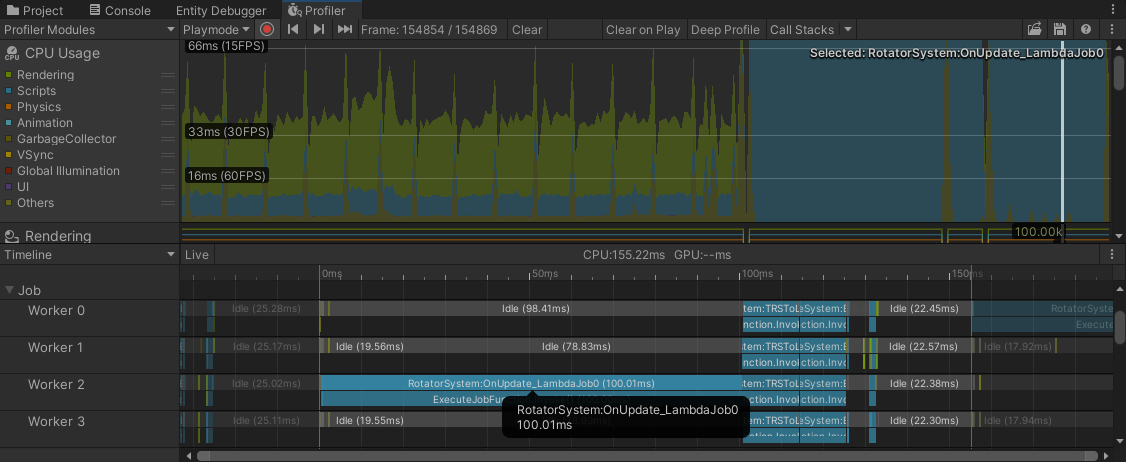
\includegraphics[width=0.95\columnwidth]{gfx/imgs/chapter5/ProfilerStressTest100k(3).png}
    \caption{Profiler: rotazione di 100.000 entità tramite scheduling di un job su un worker thread.}
    \label{fig:profiler-100k(3)}
\end{figure}

\subsubsection{ECS con job paralleli}
Come nel caso precedente, in questo test abbiamo utilizzato ECS assieme al Job System. Tuttavia, abbiamo scelto di parallelizzare ulteriormente questo meccanismo sfruttando il metodo \verb|ScheduleParallel()|. Questo metodo ci permette di distribuire il lavoro della CPU sui core secondari utilizzando i job paralleli.
Così facendo, il lavoro viene smaltito da 8 job contemporaneamente, ognuno dei quali impiega circa 147 ms per essere eseguito. Anche in questo caso, il main thread impiega circa 0,04 ms per eseguire la \verb|OnUpdate()|. Se a questo aggiungiamo una maggiore parallelizzazione, otteniamo un incremento delle prestazioni che porta l'applicazione a 13,9 FPS (Figura~\ref{fig:dati-stress-test}).

\begin{figure}[!ht]
    \centering
    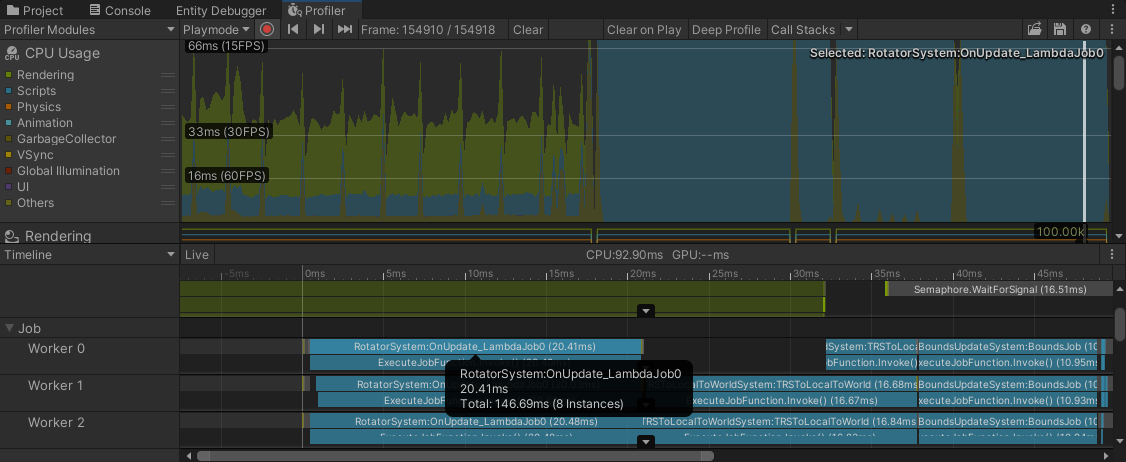
\includegraphics[width=0.95\columnwidth]{gfx/imgs/chapter5/ProfilerStressTest100k(4).png}
    \caption{Profiler: rotazione di 100.000 entità tramite job paralleli su worker thread.}
    \label{fig:profiler-100k(4)}
\end{figure}

\subsubsection{ECS con job paralleli e Burst compilation}
In questo ultimo test abbiamo sfruttato il Burst Compiler. Questo ci permette di compilare il bytecode IL/.NET dei nostri job in codice nativo estremamente performante. Infatti, semplicemente abilitando l'opzione dell'editor ``Jobs $>$ Burst $>$ Enable Compilation'', siamo riusciti ad ottenere un notevole incremento delle prestazioni: il tempo di esecuzione dei job paralleli è arrivato ad una media di circa 9,2 ms totali per 8 istanze (vedi Figura~\ref{fig:profiler-100k(5)}), mentre gli FPS a runtime sono quasi raddoppiati.

\begin{figure}[!ht]
    \centering
    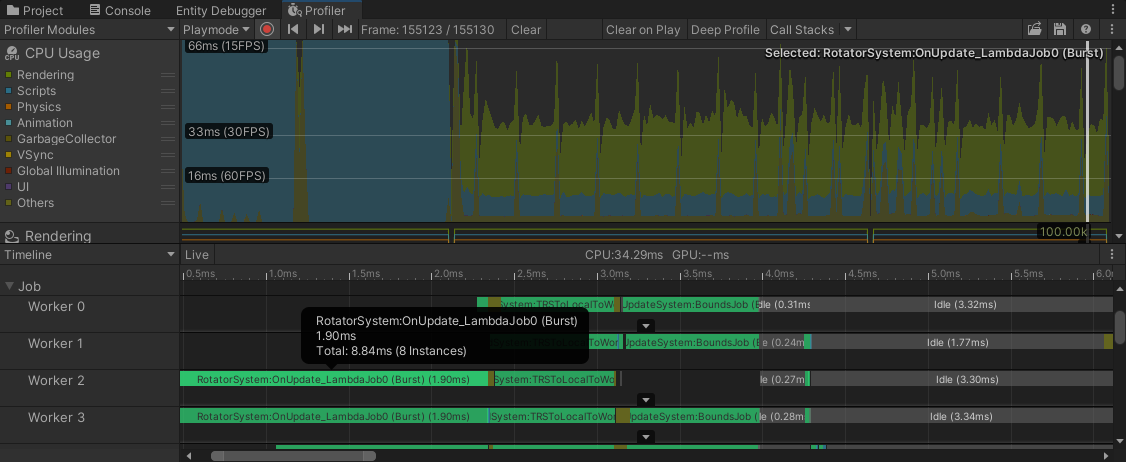
\includegraphics[width=0.95\columnwidth]{gfx/imgs/chapter5/ProfilerStressTest100k(5).png}
    \caption{Profiler: rotazione di 100.000 entità tramite job paralleli compilati con Burst su worker thread.}
    \label{fig:profiler-100k(5)}
\end{figure}


In Figura~\ref{fig:dati-fps} abbiamo riportato un grafico riassuntivo delle prestazioni in base agli FPS. In particolare, vengono paragonate tutte le implementazioni di cui abbiamo discusso in precedenza.

\begin{figure}[!ht]
    \centering
    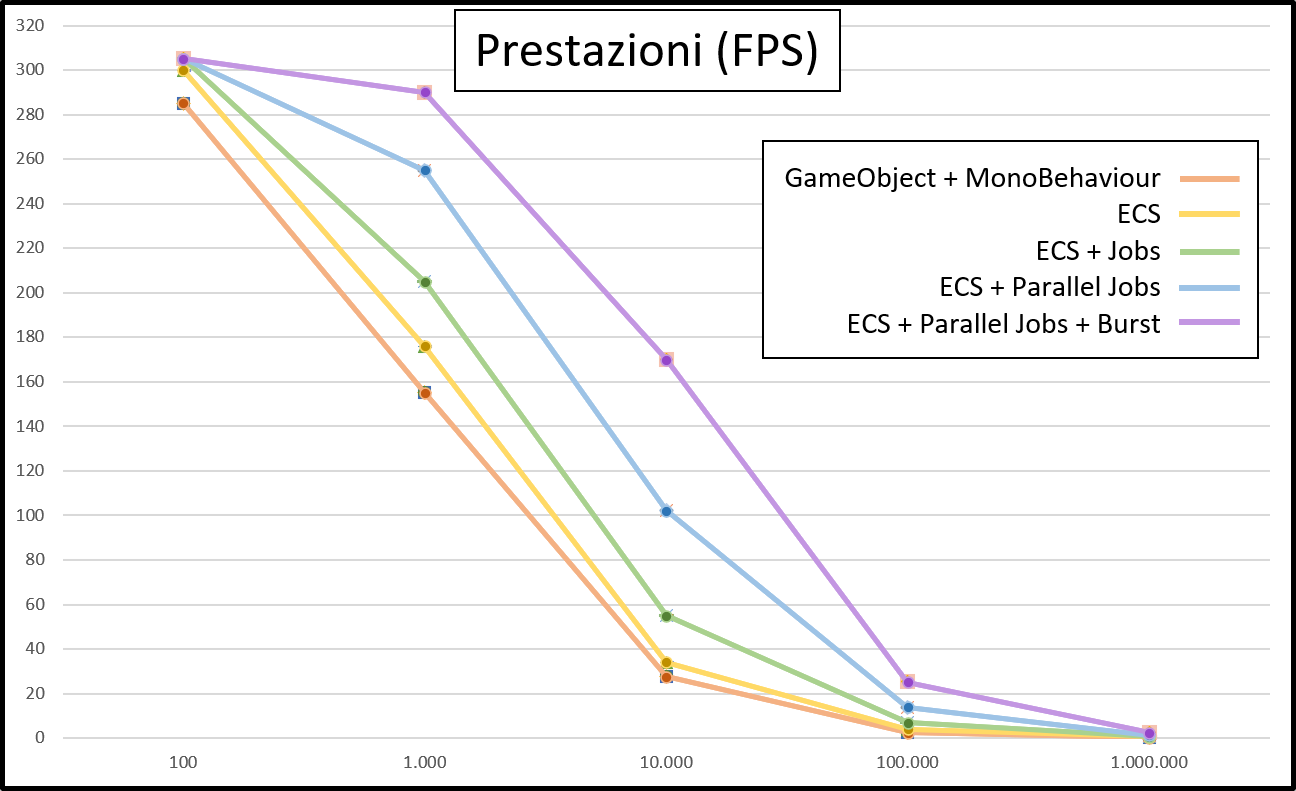
\includegraphics[width=0.95\columnwidth]{gfx/imgs/chapter5/FPSGraph.png}
    \caption{Grafico degli FPS (l'ascissa rappresenta il numero di cubi che vengono fatte ruotare, l'ordinata gli FPS relativi).}
    \label{fig:dati-fps}
\end{figure}

Dal grafico è evidente come l'utilizzo di ECS porti ad un miglioramento di prestazioni nei confronti del modello basato su GameObject. Inoltre, il divario fra le due architetture cresce all'aumentare del numero di cubi creati; soprattutto nel caso in cui utilizziamo ECS in combinazione con gli altri package.
       % 5.Risultati sperimentali
\cleardoublepage


%\phantomsection

\backmatter
\chapter*{Conclusioni e Sviluppi Futuri}
\addcontentsline{toc}{chapter}{Conclusioni e Sviluppi Futuri}

Ripercorrendo il lavoro svolto abbiamo visto inizialmente una overview sui motori di gioco, che ci ha portato alla decisione di Unity di rivoluzionare l'architettura del proprio engine. DOTS è stato introdotto con la frase \emph{performance by default}, la quale significa che con la nuova architettura non bisogna impegnarsi per realizzare del codice performante. Questo è dovuto all'efficienza del modello data-oriented su cui è basato.
Infatti, fino al 2018 Unity veniva utilizzato al massimo per applicazioni per telefono o videogiochi semplici, salvo qualche eccezione. Questo perché il modello a componenti su cui era basato si prestava molto bene per essere semplice ed user-friendly, ma era fortemente inefficiente. Di conseguenza, chi voleva realizzare un gioco più complesso solitamente optava per Unreal o qualche altro game engine.

DOTS è stato creato avendo una chiara idea di come funziona l'hardware su cui esegue il motore di gioco. Di conseguenza, sfruttando un design orientato ai dati, gli sviluppatori Unity hanno potuto realizzare un'architettura estremamente performante, basata su un modello ad entità, componenti e sistemi. 

Tramite la trattazione del package Entities, nel Capitolo~\ref{cap:ecs} abbiamo analizzato la struttura del nuovo metodo di progettare e scrivere codice di Unity, che garantisce flessibilità, separazione delle competenze e leggibilità. La sua logica basata su strutture e tipi blittable, è alla base di tutto lo stack DOTS, infatti è il package a cui è stata dedicata maggiore attenzione.

Tramite lo studio del package NetCode nel Capitolo~\ref{cap:netcode} abbiamo potuto analizzare i vari modelli di rete e le principali problematiche che possono presentarsi nello sviluppo di un gioco multiplayer. A tal proposito siamo giunti alla conclusione che il miglior pattern di networking è il modello a server autoritativo dedicato, con predizione del client. Unity ha deciso di fondare NetCode su questo modello, appunto perché è il più performante. Non a caso tipicamente viene utilizzato per videogiochi quali gli FPS, in cui è necessaria una latenza minima.

Dopo la trattazione del multigiocatore siamo passati allo sviluppo di un prototipo multigiocatore implementato interamente utilizzando i package della nuova architettura.
Lo sviluppo dei prototipi ed i risultati sperimentali ottenuti nel Capitolo~\ref{cap:risultati} ci hanno permesso di dimostrare che l'architettura classica di Unity possiede dei limiti consistenti, sia per quanto riguarda il modello su cui si basa, sia per quanto riguarda le prestazioni e la struttura del codice. In particolare, aiutandoci col Profiler Unity, abbiamo visto le diverse possibilità di miglioramento di performance, tramite l'utilizzo dei package Jobs e Burst, che ci permettono di sfruttare il multithreading. Inoltre, un utilizzo efficiente della CPU e dei suoi core, non significa solo maggiori performance, ma si traduce anche, ad esempio, in minor consumo di risorse, e maggiore durata della batteria, nel caso di applicazioni per telefono. DOTS permette di guadagnare sotto ogni punto di vista.

Al contrario, con l'approccio classico, l'utilizzo dei MonoBehaviour è molto inefficiente, in quanto, eseguendo sempre sul main thread e in sequenza, non permette di realizzare una soluzione scalabile. Inoltre, essendo un tipo riferimento, non si presta molto bene ad essere memorizzato nelle cache della CPU, all'interno delle quali occupa più spazio di quello che dovrebbe.

In conclusione, l'architettura DOTS offre un potenziale senza limiti, che può essere sfruttato per realizzare giochi e applicazioni di varia natura. Infatti, al giorno d'oggi Unity viene utilizzato non solo in ambito videoludico, ma anche in settori quali l'ingegneria ed edilizia, l'architettura, le simulazioni ed il cinema.
Per questi motivi possiamo affermare con certezza che l'assioma su cui si fonda DOTS ``performance by default'' è veritiero.

Per quanto riguarda gli sviluppi futuri, possiamo aspettarci che venga rimosso parte del codice per l'utilizzo di NetCode, il quale è leggermente prolisso e dispendioso. Probabilmente Unity continuerà il suo percorso per rendere l'architettura il più semplice possibile da usare, rimuovendo parte del codice ``boilerplate'', come ha già fatto per i job all'interno dei sistemi e la generazione automatica di comandi.
Possiamo dunque confidare che la documentazione dei vari package diventi più completa, e l'utilizzo dell'approccio data-oriented venga normalizzato, magari inserendo nell'editor qualche interfaccia specifica.

In ogni caso siamo certi che Unity continuerà lo sviluppo dello stack DOTS, fino alla release ufficiale, per la quale forse sarà necessario aspettare ancora un po'.

Per quanto riguarda il prototipo DOTS sviluppato nel capitolo~\ref{cap:prototipo}, come sviluppi futuri prevediamo di realizzare un sistema che gestisca le lobby dei giocatori, prima dell'ingresso in partita, ed un sistema di punteggio con scoreboard.
    % Conclusioni e sviluppi futuri
\cleardoublepage

%--------------%
% BIBLIOGRAFIA %
%--------------%
\addcontentsline{toc}{chapter}{\bibname}

%\nocite{gameenginearchitecture}

%\nocite{gamephysicsenginedevelopment}

\printbibliography

%References aggiuntive(?) [1] J. Gregory, Game engine architecture, second edition. CRC Press, 2014.[2] A. Kirmse, Game programming gems 4, vol. 4. Charles River Media, 2004.[3] K. Pallister, Game programming gems 5, vol. 5. Charles River Media, 2005.[4] M. Dickheiser, Game programming gems 6, vol. 6. Charles River Media, 2006.[5] M. Doherty, “A software architecture for games. % Bibliografia
\cleardoublepage

%\newpage

%%%%%%%%%%%%%%%%%%%%%%%%%%%%%%%%%%%%%%%%%%%%%%%%%%%%%%%%%%%%%%%%%%%%%%%%%%%%%
\end{document} % FINE DOCUMENTO %%%%%%%%%%%%%%%%%%%%%%%%%%%%%%%%%%%%%%%%%%%%%
%%%%%%%%%%%%%%%%%%%%%%%%%%%%%%%%%%%%%%%%%%%%%%%%%%%%%%%%%%%%%%%%%%%%%%%%%%%%%